% !TeX root = ../main.tex

% Slides
\section{Visão geral}
\begin{frame}[c]{Visão geral}
    \begin{columns}[c]
        \vspace*{-0.5cm}
        \begin{column}{0.48\linewidth}
            \begin{splusbox}{}
                \begin{itemize}
                    \item Introdução
                    \begin{itemize}
                        \item Contexto cosmológico
                        \item Estrutura em larga escala
                        \item Redshifts espectroscópicos e fotométricos
                    \end{itemize}
                    \item Objetivo
                    \item Dados
                    \begin{itemize}
                        \item Fotométricos e espectroscópicos
                        \item Pré-processamento
                        \item Pesos por objeto
                    \end{itemize}
                \end{itemize}
            \end{splusbox}
        \end{column}
        %
        \begin{column}{0.48\linewidth}
            \begin{splusbox}{}
                \begin{itemize}
                    \item Metodologia
                    \begin{itemize}
                        \item Redes neurais
                        \item Redes neurais Bayesianas
                        \item Redes de mistura de densidades
                    \end{itemize}
                    \item Resultados
                    \begin{itemize}
                        \item Redshifts fotométricos
                        \item Funções de densidade de probabilidade
                        \item Estrutura em larga escala
                    \end{itemize}
                    \item Conclusões e perspectivas
                \end{itemize}
            \end{splusbox}
        \end{column}
    \end{columns}

    % Intro
    % - LSS e cosmologia
    % - Specz e dificuldades
    % - Photoz como alternativa e métodos atuais
    % - Apresentar método ML, a BMDN

    % Objetivo
    % - Determinar photoz com a BMDN e estudar a LSS

    % Dados
    % - BMDN é supervisionada, então precisa de amostra de treino com specz
    % - Compilado specz
    % - Fotometria SPLUS
    % - Fotometria outros

    % Metodologia
    % - Intro à neurons e redes neurais
    % - BNNs
    % - MDNs
    % - BMDNs

    % Resultados
    % - SPE: apresentar métricas, resultados em bins de z ou r, resultados por campo
    % - PDF: apresentar métricas, histogramas de calibração, resultados por campo
    % - Resultados em 2D
    % - LSS: autoencoder, difusão, GNNs

    % Conclusões

    % Perspectivas
    % - Nova versão do compilado de specz
    % - Melhorias no modelo
    % - Refatoração do modelo seguindo os 4 pontos e experiência do usuário
    % - Continuidade ao projeto da LSS

\end{frame}

\section{Introdução}
% Um grande esforço no campo da astronomia é feito para caracterizar e o Universo em que vivemos. O estudo das estruturas da LSS oferece vários insights em diversos campos, de forma que a identificação de suas partes é fundamental para entender a composição, geometria, e evolução do nosso Universo.
% \begin{frame}[c]{O contexto cosmológico}
%     \begin{splusbox}{}
%         Estudar a formação e evolução da estrutura em larga escala (LSS) é fundamental para entender o Universo em que vivemos.
%     \end{splusbox}

%     \begin{splusbox}{}
%         A teoria mais aceita atualmente, chamada $\Lambda$CDM, diz que as estruturas que vemos hoje são fruto de perturbações no campo escalar primordial (o ínflaton). Estas perturbações foram amplificadas durante o período da inflação e evoluíram gravitacionalmente.
%     \end{splusbox}

%     \begin{splusbox}{}
%         Estudar estas estrutudas nos dá dicas sobre o passado e o futuro do Universo.
%     \end{splusbox}
% \end{frame}

\begin{frame}[c]{O contexto cosmológico}
    \begin{splusbox}{}
        Estudar a formação e evolução da estrutura em larga escala (LSS) é fundamental para entender o Universo em que vivemos. A partir dela podemos ter insights sobre:
        \begin{itemize}
            \item Matéria escura
            \item Energia escura
            \item Evolução cósmica
            \item Formação e evolução de galáxias
            \item Física a nível fundamental
        \end{itemize}
    \end{splusbox}
\end{frame}

\begin{frame}[c]{Estrutura em larga escala}
    A teia cósmica, ou a LSS, é formada por diferentes componentes. Cada componente apresenta caracteristicas e possui papéis diferentes na evolução do Universo como um todo.

    \begin{figure}
        \centering
        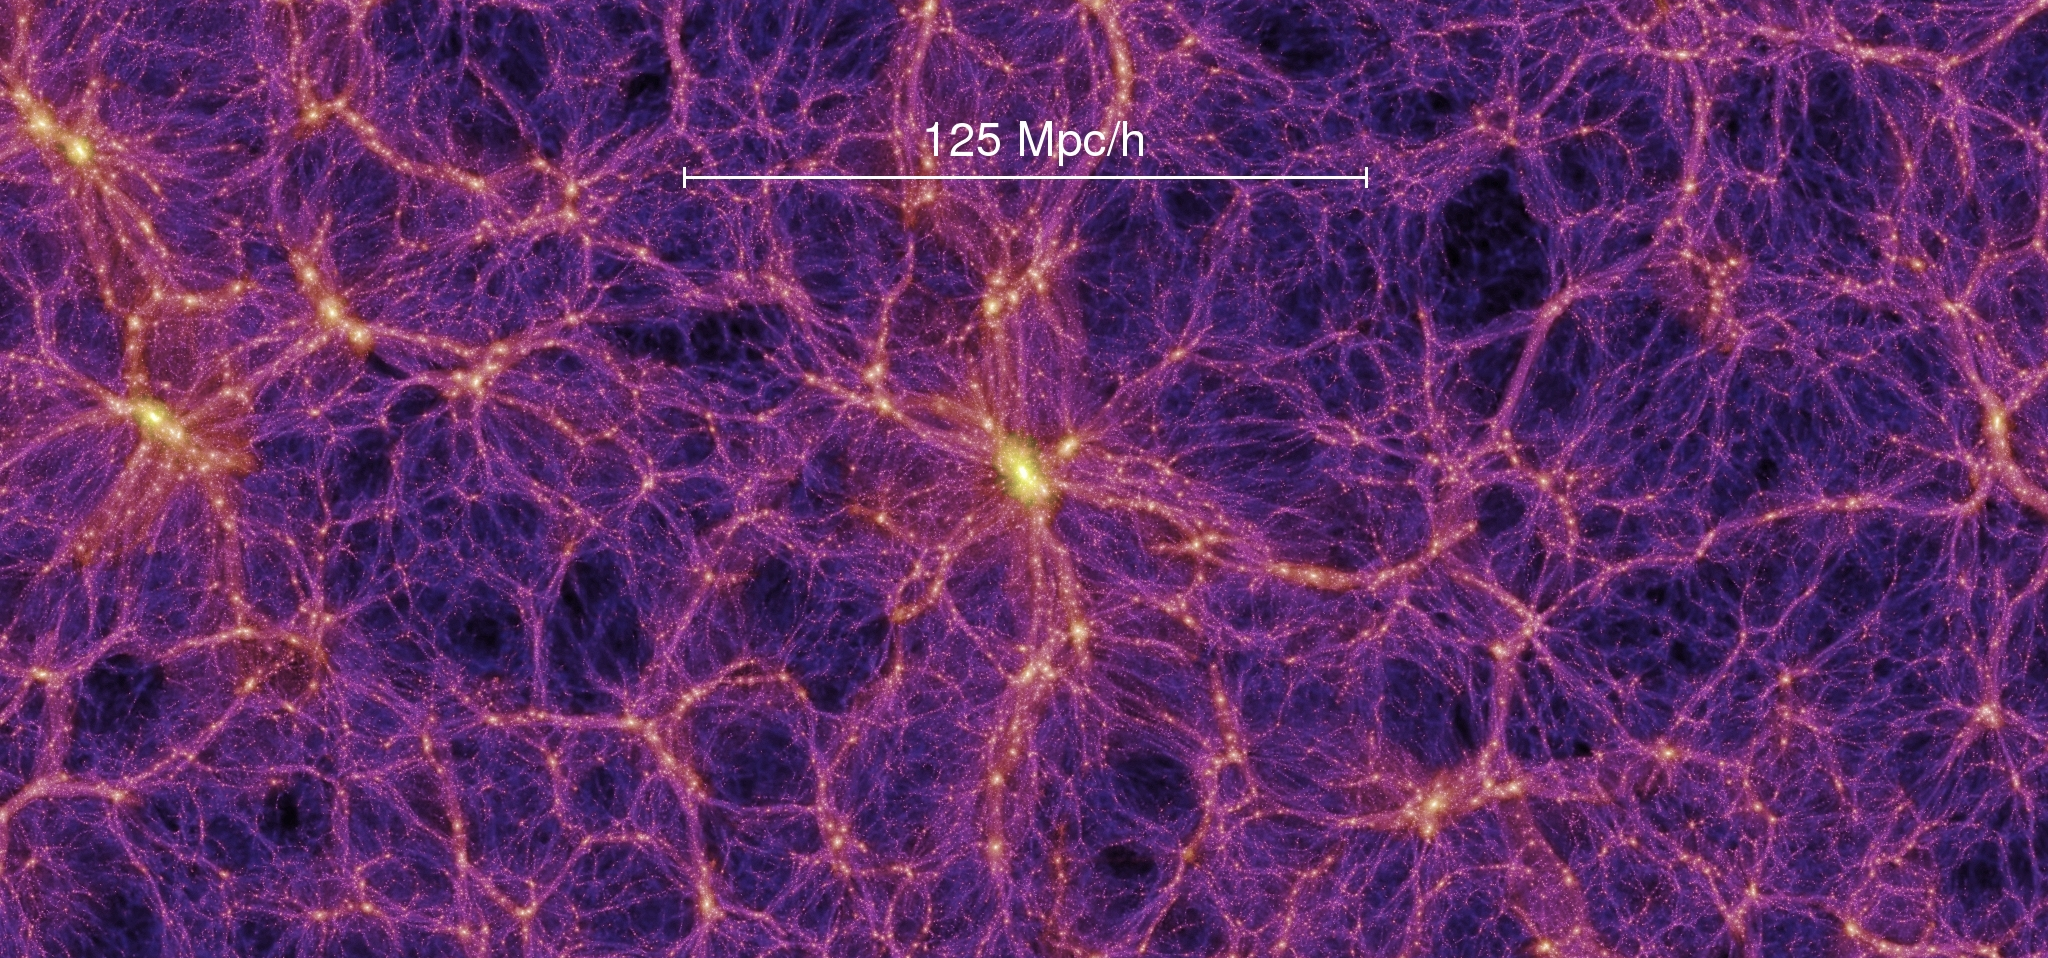
\includegraphics[height=5cm]{script/images/millenium.png}
        \caption{Adaptado de \url{https://wwwmpa.mpa-garching.mpg.de/galform/virgo/millennium/}.}
    \end{figure}

    % \begin{columns}
    %     \begin{column}{0.32\linewidth}
    %         \begin{splusbox}{Filamentos}
                
    %         \end{splusbox}
    %     \end{column}
    %     %
    %     \begin{column}{0.32\linewidth}
    %         \begin{splusbox}{Aglomerados}
                
    %         \end{splusbox}
    %     \end{column}
    %     %
    %     \begin{column}{0.32\linewidth}
    %         \begin{splusbox}{Vazios}
                
    %         \end{splusbox}
    %     \end{column}
    % \end{columns}
\end{frame}

\begin{frame}[c]{Estrutura em larga escala}
    \begin{figure}
        \centering
        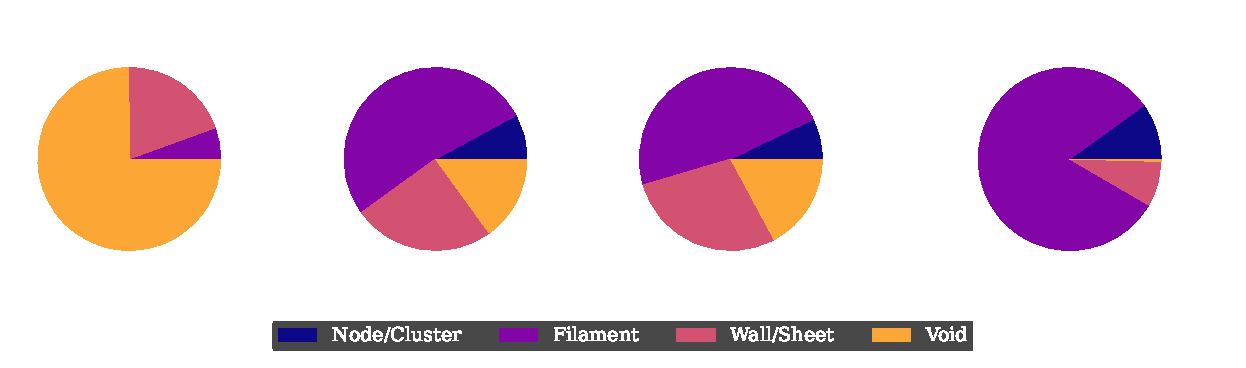
\includegraphics[width=\linewidth]{script/images/lss_distribution.pdf}
        \caption{Adaptado de: Ganeshaiah Veena et al. (2019).}
    \end{figure}
\end{frame}

\begin{frame}[c]{Estrutura em larga escala}
    \begin{columns}[c]
        \begin{column}{0.56\textwidth}
            \begin{figure}
                \centering
                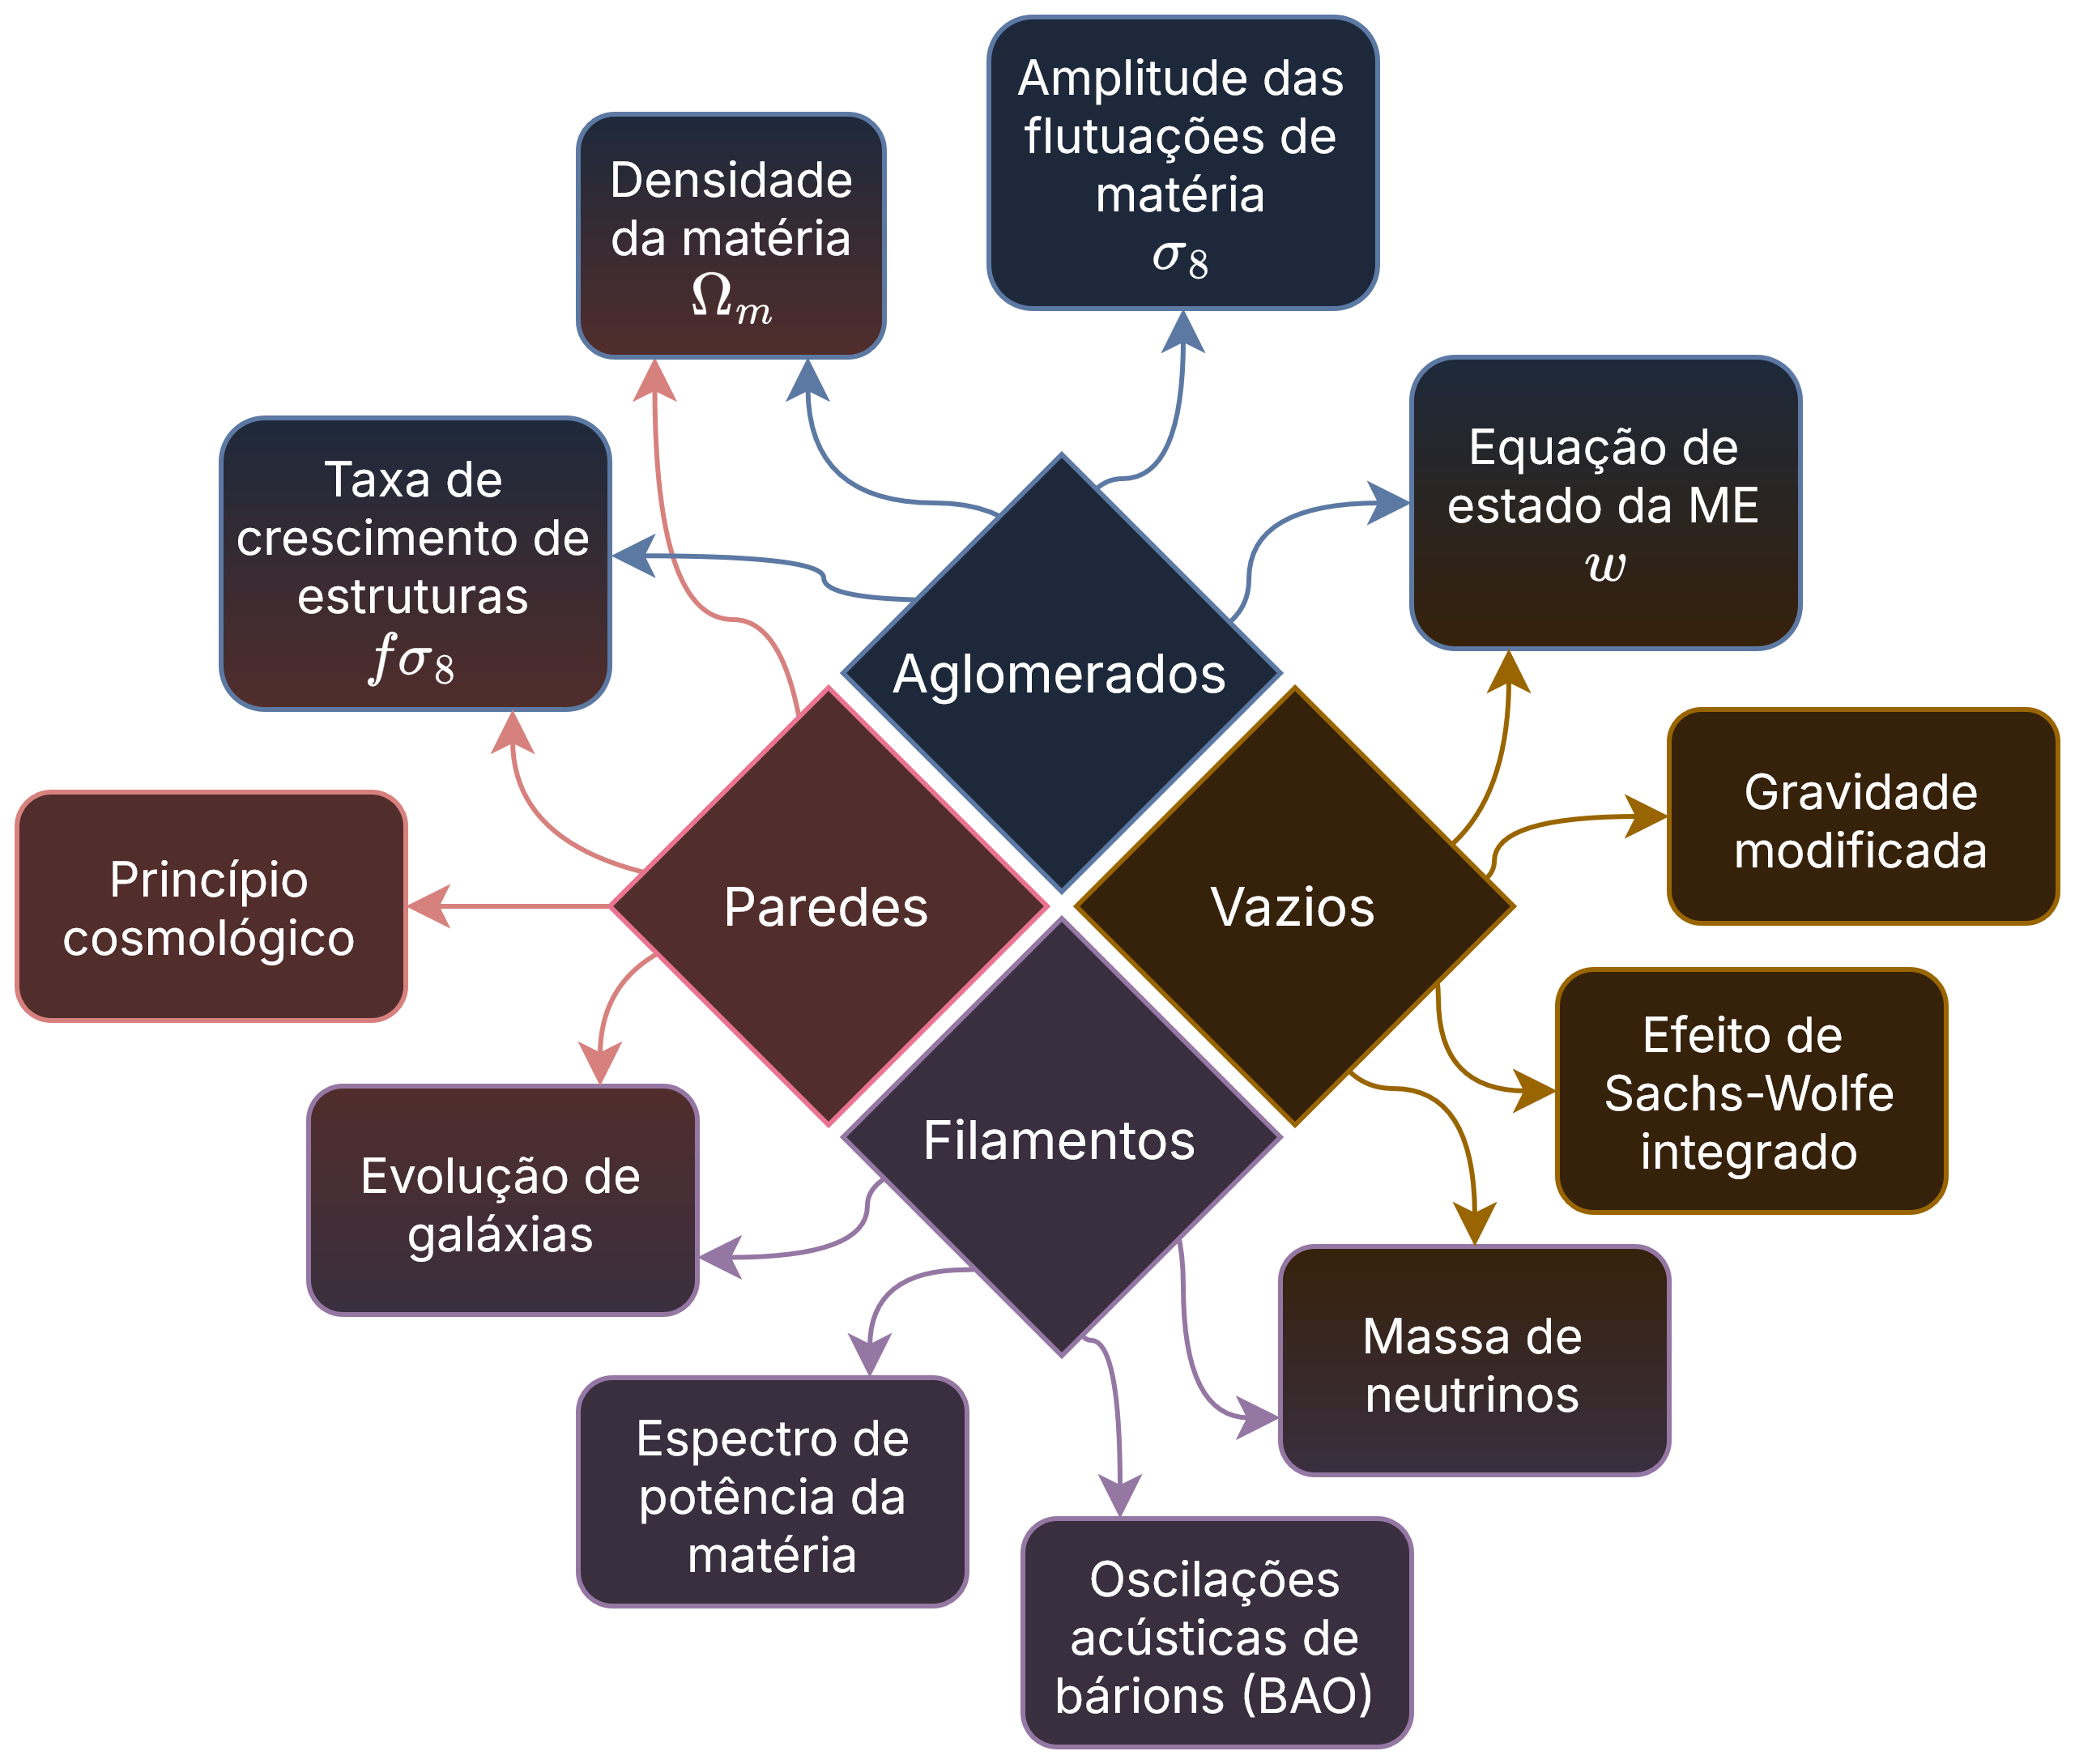
\includegraphics[height=7cm]{images/LSS.png}
            \end{figure}
        \end{column}
        %
        \begin{column}{0.36\textwidth}
            \begin{splusbox}{}
                O problema é que estas estruturas são tridimensionais, mas nossas observações são projetadas (bidimensionais)
            \end{splusbox}
        \end{column}
    \end{columns}
\end{frame}

% \begin{frame}[c]{Estrutura em larga escala}
%     \begin{figure}
%         \centering
%         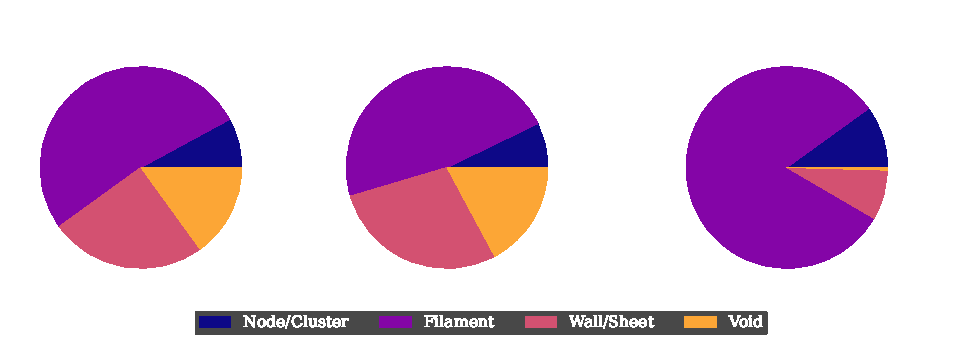
\includegraphics[width=\linewidth]{script/images/lss_mass_distribution.pdf}
%     \end{figure}
%     %
%     \begin{splusbox}{}
%         \centering
%         O problema é que estas estruturas são tridimensionais, mas nossas observações são projetadas (bidimensionais)
%     \end{splusbox}
% \end{frame}

% \begin{frame}[c]{Redshifts espectroscópicos e suas limitações}
%     Uma forma de determinar a distância de objetos celestes vêm da lei de Hubble Lemaître:
%     \begin{equation*}
%         v_\text{res} = c \cdot z = H_0 \cdot D,
%     \end{equation*}
%     sendo $z$ o redshift, medida que obtemos a partir da observação do espectro de um objeto.
%     %
%     \begin{splusbox}{}
%         \centering
%         A observação de um espectro com alto sinal ruído demanda bastante tempo de observação, ainda mais para objetos fracos
%         \vspace{0.3cm}
%         É necessário encontrar uma alternativa
%     \end{splusbox}
% \end{frame}

\begin{frame}[c]{Redshifts espectroscópicos e suas limitações}
    Uma forma de determinar a distância de objetos celestes vêm da lei de Hubble Lemaître (válida para objetos próximos):
    \vspace*{-0.5cm}
    \begin{figure}
        \centering
        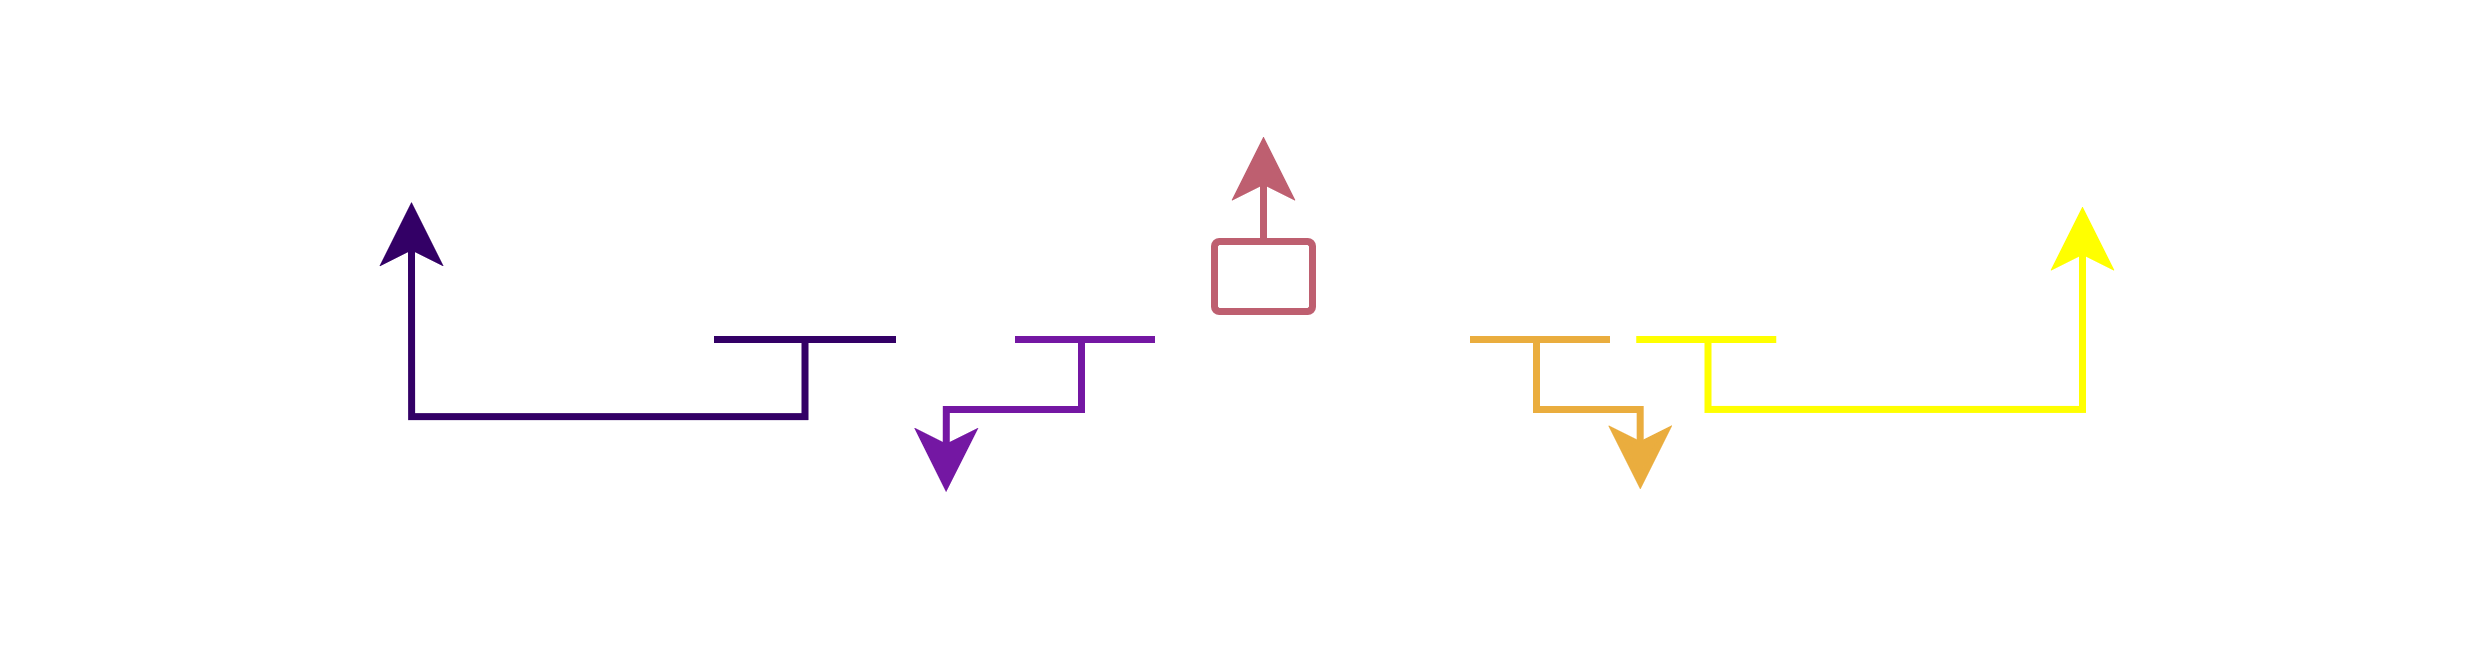
\includegraphics[width=0.8\linewidth]{script/images/hubble_law.png}
    \end{figure}
    \vspace*{-0.5cm}
    \begin{splusbox}{}
        \centering
        A observação de um espectro com alto sinal ruído demanda bastante tempo de observação, ainda mais para objetos fracos

        \vspace{0.3cm}
        É necessário encontrar uma alternativa
    \end{splusbox}
\end{frame}

\begin{frame}[c]{A alternativa: redshifts fotométricos}
    %\hspace*{1cm}
    \begin{columns}[c]
        \begin{column}{0.46\linewidth}
            \justifying
            Existem uma série de projetos que se baseiam em fotometria para produzir ciência.
            \begin{itemize}
                \justifying
                \item Pode ser considerada uma "aproximação" do espectro
                \item É obtida de forma muito mais rápida
                \item Pode alcançar magnitudes mais fracas
                \item É capaz de gerar dados para muitos objetos e grandes áreas
            \end{itemize}
        \end{column}
        \hspace*{-0.5cm}
        \begin{column}{0.46\linewidth}
            \begin{figure}
                \centering
                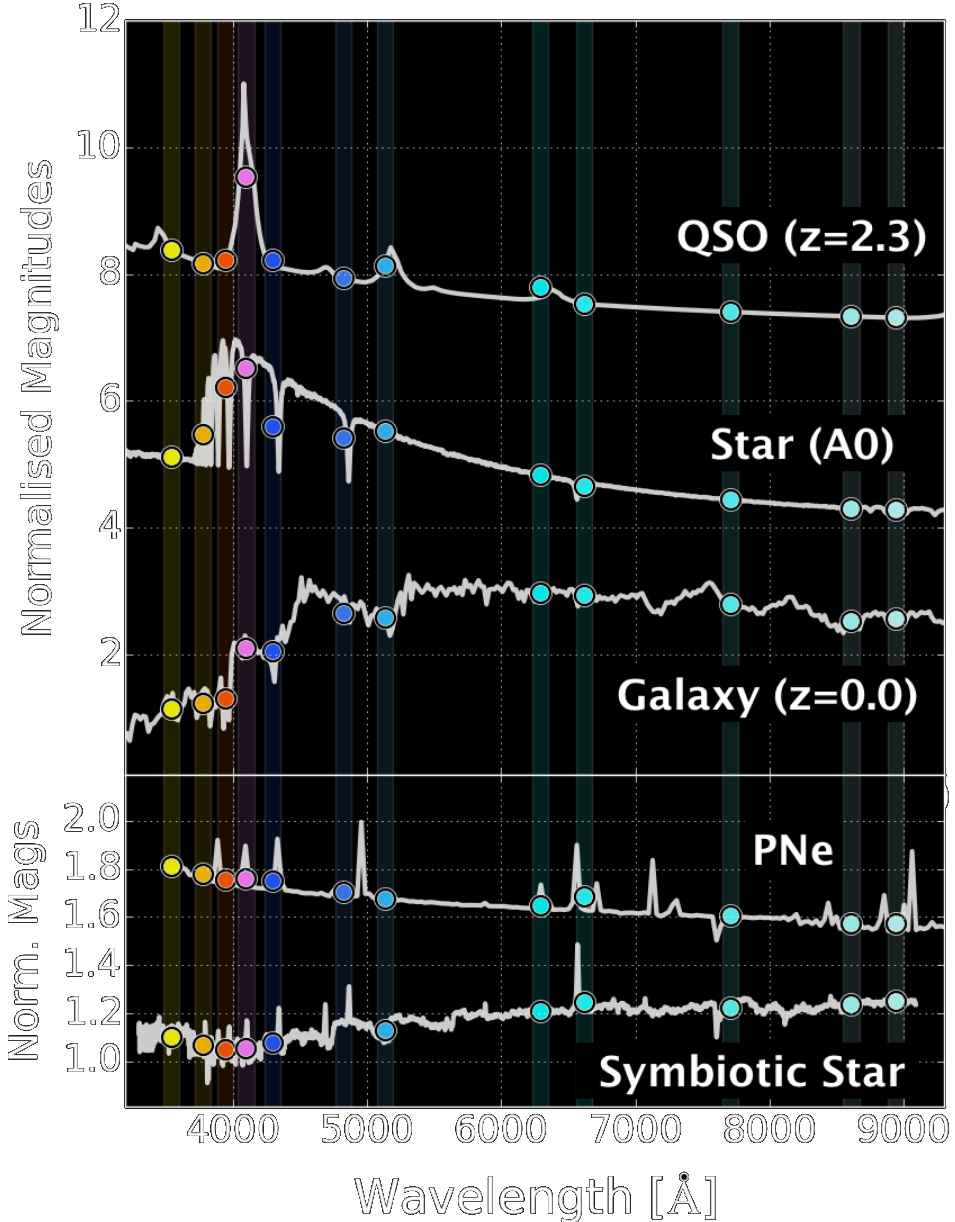
\includegraphics[height=5.5cm]{script/images/splus_spectra_sed.png}
                \caption{Adaptado de: Mendes de Oliveira et al. (2019).}
            \end{figure}
        \end{column}
    \end{columns}
\end{frame}

\begin{frame}[c]{A alternativa: redshifts fotométricos}
    Redshifts fotométricos são estimados por três tipos de algoritmos: aprendizado de máquina, ajuste de templates e códigos híbridos.

    \begin{columns}[c]
        \footnotesize
        \begin{column}{0.46\textwidth}
            \begin{splusbox}{Aprendizado de máquina (ML)}
                \begin{itemize}
                    \justifying
                    \item[$\checkmark$] Se baseiam no uso de uma amostra de treinamento
                    \item[$\checkmark$] Flexível em relação a modelos (RFs, KNNs, SVMs)
                    \item[$\checkmark$] Podem ser mais precisos e rápidos que modelos de ajuste de template
                    \item[$\times$] Não fornecem uma classificação do objeto (exceto caso seja configurado para isso)
                    \item[$\times$] Sujeito à vieses devido aos dados
                \end{itemize}
            \end{splusbox}
        \end{column}

        \begin{column}{0.46\textwidth}
            \begin{splusbox}{Ajuste de templates (TF)}
                \begin{itemize}
                    \justifying
                    \item[$\checkmark$] Fazem uma comparação entre a fotometria de um objeto e uma biblioteca de templates
                    \item[$\checkmark$] Fornecem uma classificação do objeto junto ao $z_\text{phot}$
                    \item[$\checkmark$] Maior capacidade de extrapolação
                    \item[$\times$] Menos precisos, mais lentos
                    \item[$\times$] Sujeito à vieses devido à escolha dos templates
                \end{itemize}
            \end{splusbox}
        \end{column}

        % \begin{column}{0.33\linewidth}
        %     \begin{splusbox}{Híbridos}
        %         \footnotesize
        %         \begin{itemize}
        %             \item Combinam características de ML e TF
        %             \item Alguns códigos usam ML para gerar templates para um código de TF, outros usam templates para criar dados a serem usados num modelo de ML
        %         \end{itemize}
        %     \end{splusbox}
        % \end{column}
    \end{columns}
\end{frame}

\section{O objetivo}
% O nosso objetivo é simples. Usando as bandas estreitas do SPLUS, queremos fornecer dados que sirvam como uma interface entre a alta precisão dos surveys espectroscópicos e a versatilidade dos surveys fotométricos, permitindo um mapeamento de alta precisão e econômico das estruturas da LSS através do tempo cósmico, suplementando os dados espectroscópicos expandindo o alcance em redshift e o tamanho das amostras, ao mesmo tempo que nós mitigamos as limitações impostas por surveys fotométricos de bandas largas.
\begin{frame}[c]{O objetivo}
    \begin{columns}[c]
        \begin{column}{0.46\linewidth}
            \begin{splusbox}{Redshifts fotométricos}
                \begin{itemize}
                    \justifying
                    \item Determinação de redshifts fotométricos de alta precisão
                    \item Funções de densidade de probabilidade bem calibradas
                    \item Galáxias até $z=0.8$ e magnitude 21 na banda \texttt{r}
                \end{itemize}
            \end{splusbox}
        \end{column}
        \begin{column}{0.46\linewidth}
            \begin{splusbox}{Estrutura em larga escala}
                \begin{itemize}
                    \justifying
                    \item Utilizar dados fotométricos para a reconstrução da LSS
                    \item Obter um mapeamento similar ao visto usando $z_\text{spec}$
                    %\item Possibilitar estudos que abrangem diferentes áreas da cosmologia
                \end{itemize}
                %Recuperação das estrutura da LSS, tal como vemos usando $z_\text{spec}$, a partir de estimativas fotométricas
            \end{splusbox}
        \end{column}
    \end{columns}

    \centering
    \begin{splusbox}{}
        Expandir o conjunto de dados que podemos usar para estudos em diferentes áreas da astronomia
    \end{splusbox}
\end{frame}

\section{Dados}
% \begin{frame}[c]{Dados espectroscópicos}
%     5097 catálogos foram baixados do VizieR, HEASARC, SDSS, entre outros, dos quais 1852 foram usados para criar o compilado.

%     \begin{figure}
%         \centering
%         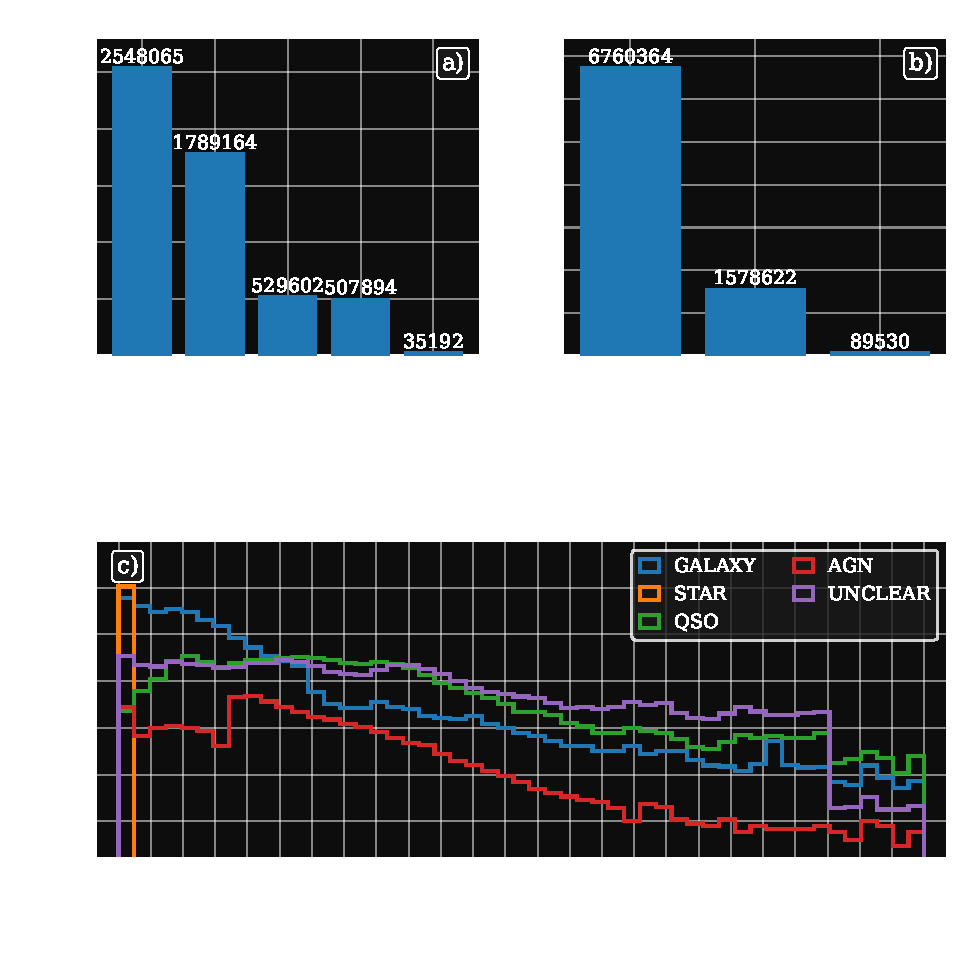
\includegraphics[height=5.5cm]{script/images/specz_distributions.pdf}
%     \end{figure}

% \end{frame}

\begin{frame}[c]{Dados fotométricos}
    % O foco deste trabalho está no SPLUS, pois esta é a fonte principal de dados.
    % %
    \begin{figure}
        \centering
        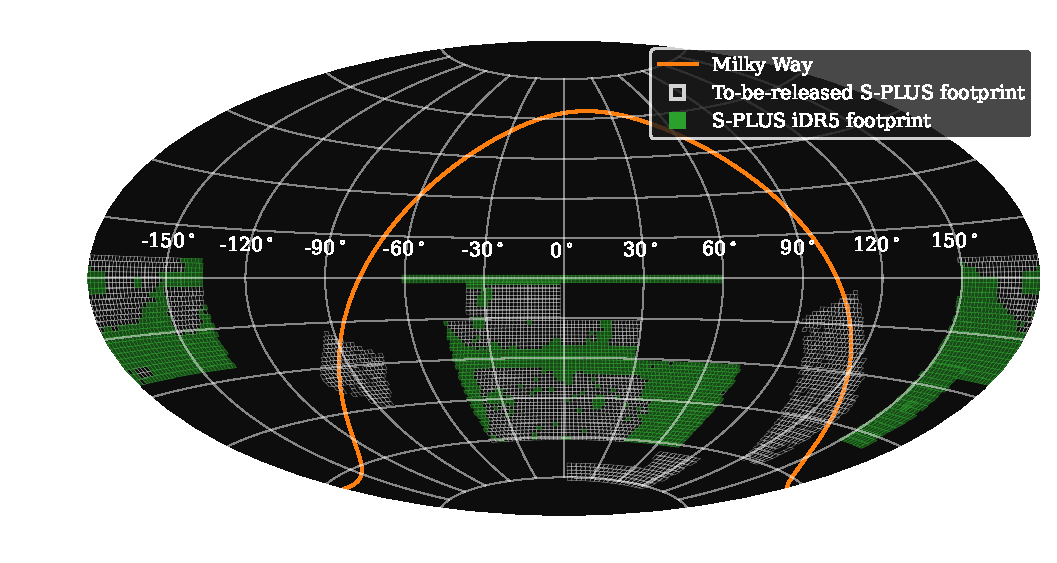
\includegraphics[height=7cm]{script/images/splus_footprint_idr5.pdf}
    \end{figure}
\end{frame}

% \begin{frame}[c]{Dados fotométricos}%[label=current]

%     \begin{columns}[c]
%         \begin{column}{0.32\textwidth}
%             \begin{table}[h]
%                 \tiny
%                 \centering
%                 \label{tab:filters}
%                   \begin{tabular}{@{}lccc@{}}
%                       \toprule
%                       \textbf{Filter} & \textbf{Survey} & \textbf{Effective $\lambda$} & \textbf{Depth (typical, AB mags)} \\ \midrule % & \textbf{Number of sources} \\ \midrule
%                       FUV             & \multirow{2}{*}{GALEX}       & \qty{1548.85}{\angstrom}     & 19.9                 \\ % &                            \\
%                       NUV             &                              & \qty{2303.37}{\angstrom}     & 20.8                 \\ \midrule % &                            \\ \midrule
%                       u$_\text{JAVA}$ & \multirow{12}{*}{S-PLUS}     & \qty{3542.07}{\angstrom}     & 20.83                \\ % &                            \\
%                       J0378           &                              & \qty{3783.69}{\angstrom}     & 20.19                \\ % &                            \\
%                       J0395           &                              & \qty{3940.17}{\angstrom}     & 19.67                \\ % &                            \\
%                       J0410           &                              & \qty{4094.63}{\angstrom}     & 19.78                \\ % &                            \\
%                       J0430           &                              & \qty{4286.52}{\angstrom}     & 19.82                \\ % &                            \\
%                       g$_\text{SDSS}$ &                              & \qty{4715.83}{\angstrom}     & 21.10                \\ % &                            \\
%                       J0515           &                              & \qty{5131.93}{\angstrom}     & 20.05                \\ % &                            \\
%                       r$_\text{SDSS}$ &                              & \qty{6202.57}{\angstrom}     & 21.18                \\ % &                            \\
%                       J0660           &                              & \qty{6616.95}{\angstrom}     & 20.98                \\ % &                            \\
%                       i$_\text{SDSS}$ &                              & \qty{7627.01}{\angstrom}     & 20.79                \\ % &                            \\
%                       J0861           &                              & \qty{8607.17}{\angstrom}     & 19.78                \\ % &                            \\
%                       z$_\text{SDSS}$ &                              & \qty{8913.47}{\angstrom}     & 20.03                \\ \midrule % &                            \\ \midrule
%                       Y               & \multirow{4}{*}{VHS}         & \qty{1.021}{\micro\metre}    & 21.1                 \\ % &                            \\
%                       J               &                              & \qty{1.254}{\micro\metre}    & 20.8                 \\ % &                            \\
%                       H               &                              & \qty{1.646}{\micro\metre}    & 20.5                 \\ % &                            \\
%                       Ks              &                              & \qty{2.149}{\micro\metre}    & 20.0                 \\ \midrule % &                            \\ \midrule
%                       W1              & \multirow{2}{*}{WISE}        & \qty{3.368}{\micro\metre}    & 20.72                \\ % &                            \\
%                       W2              &                              & \qty{4.618}{\micro\metre}    & 19.97                \\ % &                            \\
%                       \bottomrule
%                   \end{tabular}
%               \end{table}
%         \end{column}

%         \begin{column}{0.65\textwidth}
%             \begin{figure}
%                 \centering
%                 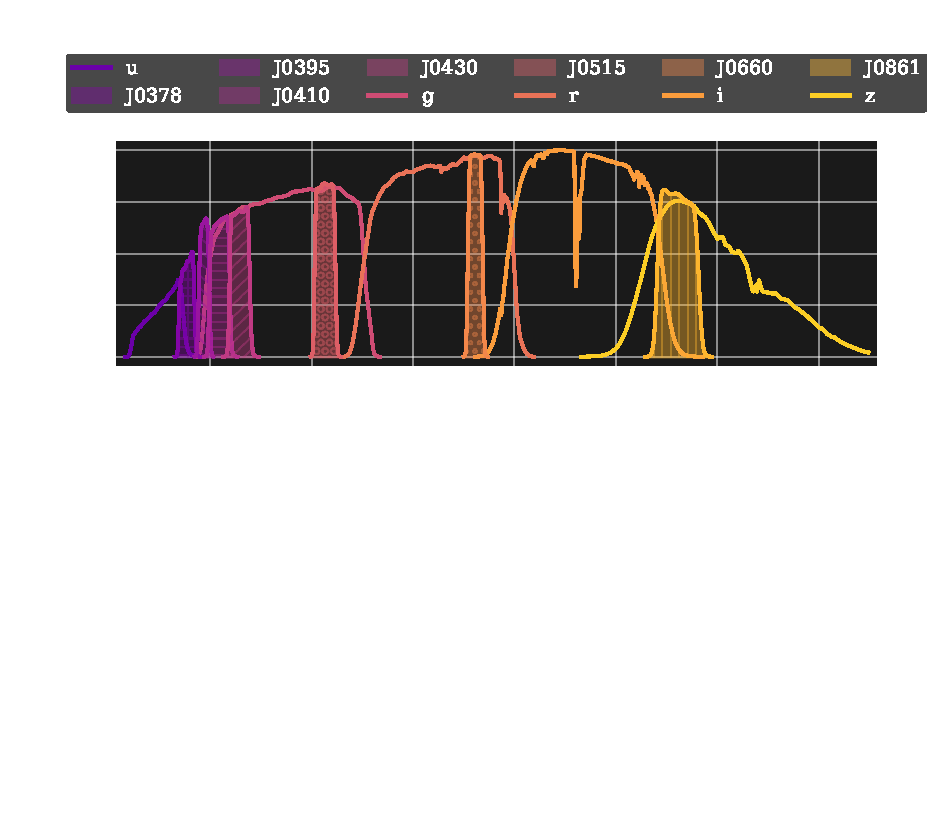
\includegraphics[height=6.5cm]{script/images/transmission_curves.pdf}
%             \end{figure}
%         \end{column}
%     \end{columns}

% \end{frame}

\begin{frame}[c]{Dados fotométricos}%[label=current]
    \begin{figure}
        \centering
        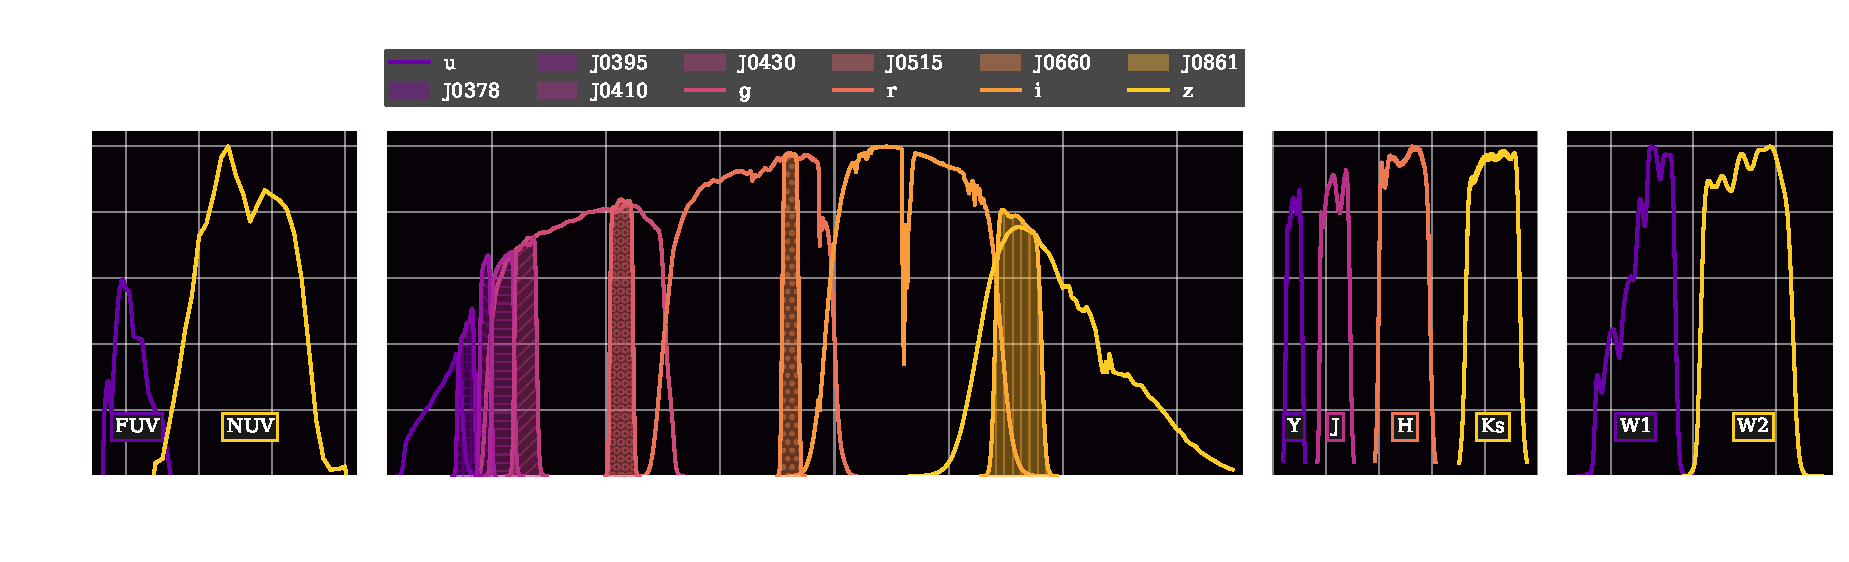
\includegraphics[width=\linewidth]{script/images/transmission_curves_2.pdf}
    \end{figure}
\end{frame}

\begin{frame}[c]{Dados fotométricos}
    \begin{figure}
        \centering
        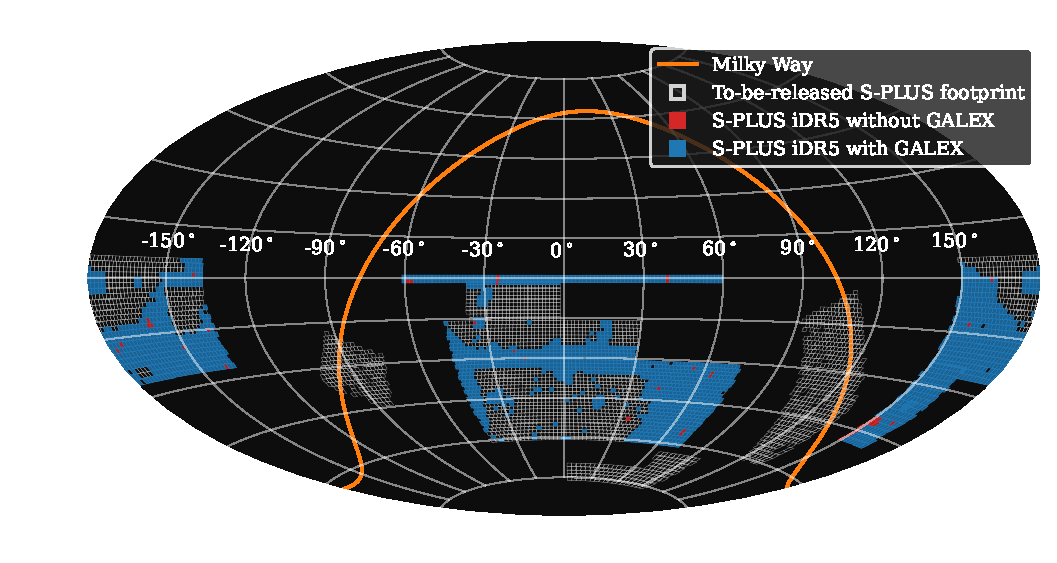
\includegraphics[height=7cm]{script/images/splus_footprint_idr5_GALEX.pdf}
    \end{figure}
\end{frame}

\begin{frame}[c]{Dados fotométricos}
    \begin{figure}
        \centering
        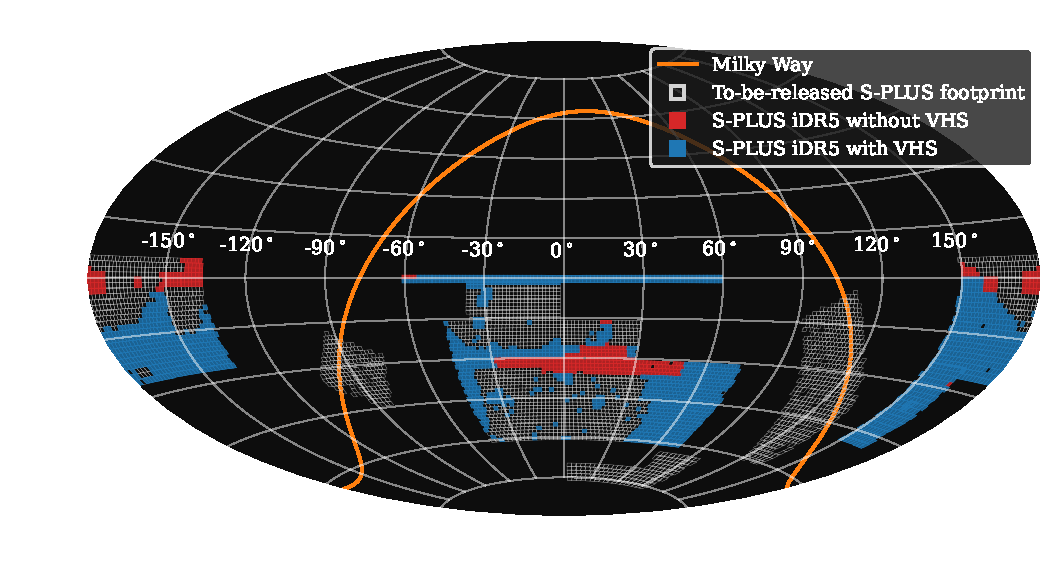
\includegraphics[height=7cm]{script/images/splus_footprint_idr5_VHS.pdf}
    \end{figure}
\end{frame}

\begin{frame}[c]{Dados fotométricos}
    \begin{figure}
        \centering
        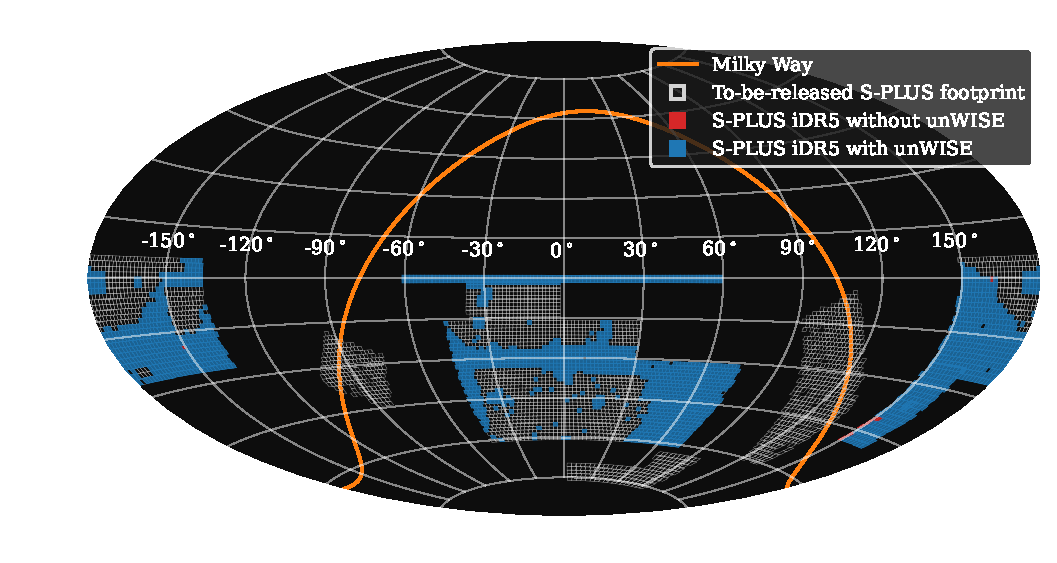
\includegraphics[height=7cm]{script/images/splus_footprint_idr5_unWISE.pdf}
    \end{figure}
\end{frame}

\begin{frame}[c]{Dados fotométricos}
    \begin{figure}
        \centering
        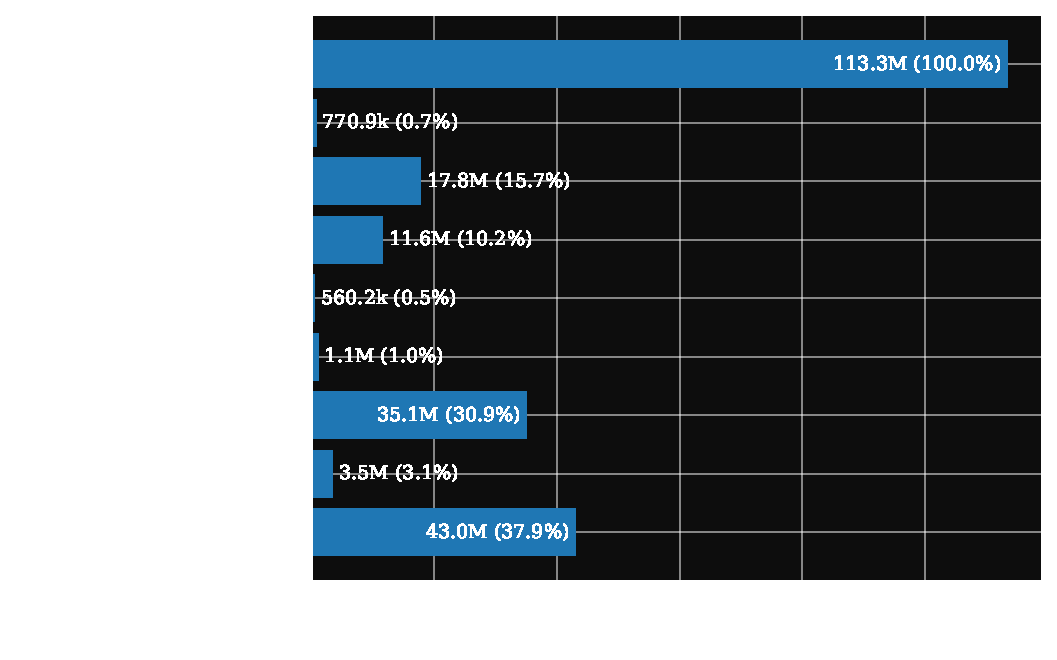
\includegraphics[height=6.5cm]{script/images/crossmatch_stats.pdf}
    \end{figure}
\end{frame}

\begin{frame}{Dados espectroscópicos {\small \textcolor{gray}{\url{(https://github.com/ErikVini/specz_compilation)}}}}
    \begin{columns}[c]
        \hspace{0.5cm}
        \begin{column}{0.40\textwidth}
            \begin{splusbox}{Informações do compilado}
                \begin{itemize}
                    \item Total de catálogos: 5097
                    \item Catálogos usados: 1872
                    \item Total de objetos: \mbox{8 437 460}
                    \item \underline{Pré era GPT!}
                \end{itemize}
            \end{splusbox}
        \end{column}
        %\hspace{-0.5cm}
        \begin{column}{0.50\textwidth}
            \begin{figure}
                \centering
                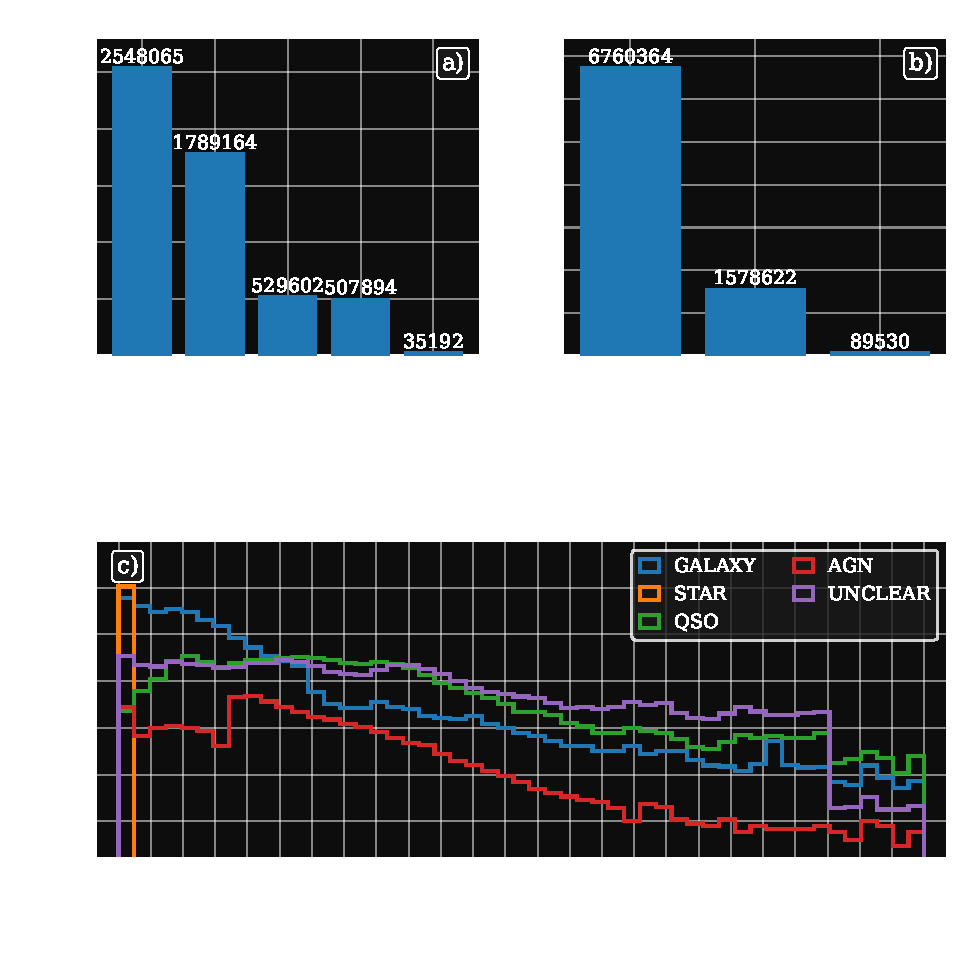
\includegraphics[height=7cm]{script/images/specz_distributions.pdf}
            \end{figure}
        \end{column}
    \end{columns}
\end{frame}

\begin{frame}[c]{Dados espectroscópicos}
    \begin{figure}
        \centering
        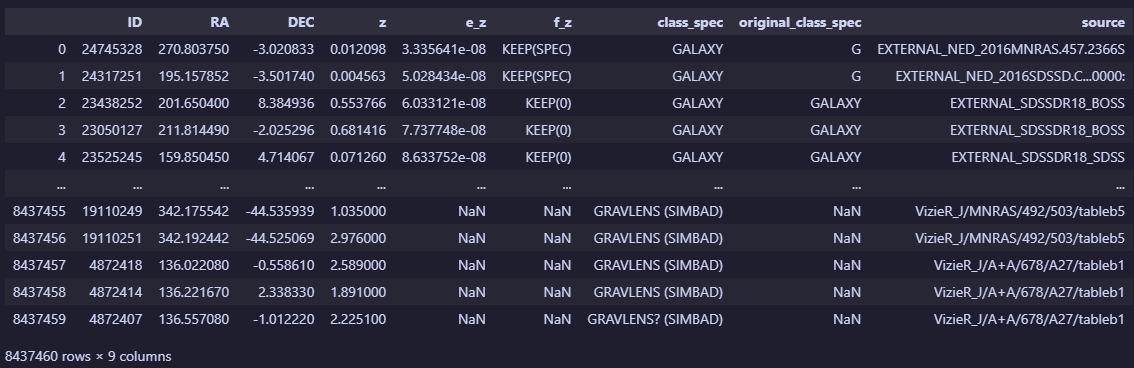
\includegraphics[width=\linewidth]{script/images/specz_compilation.png}
    \end{figure}
\end{frame}

\begin{frame}[c]{Dados espectroscópicos}
    \begin{figure}
        \centering
        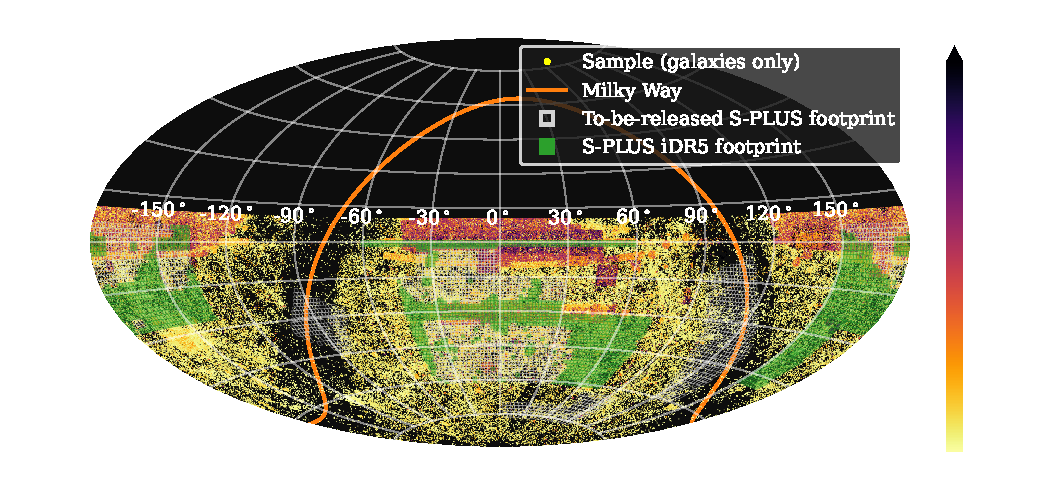
\includegraphics[height=6.5cm]{script/images/spectroscopic_compilation.pdf}
    \end{figure}
\end{frame}

% \begin{frame}[c]{Criando os catálogos}
%     \begin{columns}[c]
%         \begin{column}{0.49\textwidth}
%             \begin{splusbox}{Crossmatches espectroscópicos}
%                 bla
%             \end{splusbox}
%         \end{column}

%         \begin{column}{0.49\textwidth}
%             \begin{splusbox}{Crossmatches fotométricos}
%                 bla
%             \end{splusbox}
%         \end{column}
%     \end{columns}
% \end{frame}

% \begin{frame}[c]{Criando os catálogos}
%     \begin{splusbox}{Crossmatches espectroscópicos}
%         Busca radial (RA, DEC) com raio de 2'' em torno de cada objeto do SPLUS
%     \end{splusbox}
% \end{frame}

% \begin{frame}[c]{Criando os catálogos}
%     \begin{splusbox}{Crossmatches fotométricos}
%         GALEX:
%         \begin{itemize}
%             \item Busca radial (RA, DEC) com raio de 2'' em torno de cada objeto do SPLUS
%             \item Conversão entre magnitudes Vega para AB
%         \end{itemize}
%         VHS:
%         \begin{itemize}
%             \item Busca radial (RA, DEC) com raio de 1'' em torno de cada objeto do SPLUS
%             \item Conversão entre magnitudes Vega para AB
%         \end{itemize}
%         unWISE:
%         \begin{itemize}
%             \item Busca radial (RA, DEC) com raio de 1'' em torno de cada objeto do SPLUS
%             \item Conversão entre magnitudes Vega para AB
%             \item Cálculo dos valores de erros nas mangitudes
%         \end{itemize}
%     \end{splusbox}
% \end{frame}

\begin{frame}[c]{Criando o catálogo para treinamento}
    \begin{splusbox}{Crossmatches espectroscópicos}
        \small
        Busca radial (RA, DEC) com raio de 2" em torno de cada objeto do SPLUS
    \end{splusbox}
    \begin{splusbox}{Crossmatches fotométricos}
        \small
        \begin{columns}[t]
            \begin{column}{0.29\textwidth}
               GALEX \textcolor{LightGray}{(II/335/galex\_ais)}:
               \begin{itemize}
                    \item Busca radial com raio de 2"
                \end{itemize}
            \end{column}
            \begin{column}{0.29\textwidth}
                VHS \textcolor{LightGray}{(II/367/vhs\_dr5)}:
                \begin{itemize}
                    \justifying
                    \item Busca radial com raio de 1"
                    \item Conversão de magnitudes Vega para AB
                \end{itemize}
            \end{column}
            \begin{column}{0.29\textwidth}
                unWISE \textcolor{LightGray}{(II/363/unwise)}:
                \begin{itemize}
                    \justifying
                    \item Busca radial com raio de 1"
                    \item Cálculo das magnitudes e erros
                    \item Conversão de magnitudes Vega para AB
                \end{itemize}
            \end{column}
        \end{columns}
    \end{splusbox}
\end{frame}

\begin{frame}[c]{Pré-processamento}
    \begin{columns}[c]
        \begin{column}{0.56\linewidth}
            \vspace{0.2cm}
            \begin{table}
                \centering
                \label{tab:constraints}
                  \begin{tabular}{@{}ll@{}}
                      \toprule
                      \textbf{Variable}        & \textbf{Constraints}                              \\ \midrule
                      \texttt{r\_auto}         & {[}14, 21{]}                                      \\
                      \texttt{nDet\_PStotal}   & $\geqslant$ 1                                     \\
                      \texttt{SEX\_FLAGS\_DET} & {[}0, 3{]}                                        \\ \midrule
                      \texttt{z}               & {[}0.002, 0.8{]}                                    \\
                      \texttt{e\_z}            & $\leqslant$ 0.002                                 \\
                      \texttt{f\_z}            & not \ttt{REMOVE}                                  \\
                      \texttt{class\_spec}     & \ttt{GALAXY}, \ttt{SUPERNOVAE} or \ttt{AGN}       \\
                      Separation               & $\leqslant$ 1''                                   \\ \bottomrule
                  \end{tabular}
              \end{table}
        \end{column}
        %
        %\hspace*{-2cm}
        \begin{column}{0.36\linewidth}
            \begin{splusbox}{}
                \begin{itemize}
                    \justifying
                    \item Galáxias
                    \item Nem muito fracas, nem muito brilhantes
                    \item Com boa fotometria
                    \item Com redshifts de boa qualidade e entre 0.002 e 0.8
                \end{itemize}
            \end{splusbox}
        \end{column}
    \end{columns}
\end{frame}

\begin{frame}[c]{Pré-processamento}
    \begin{figure}
        \centering
        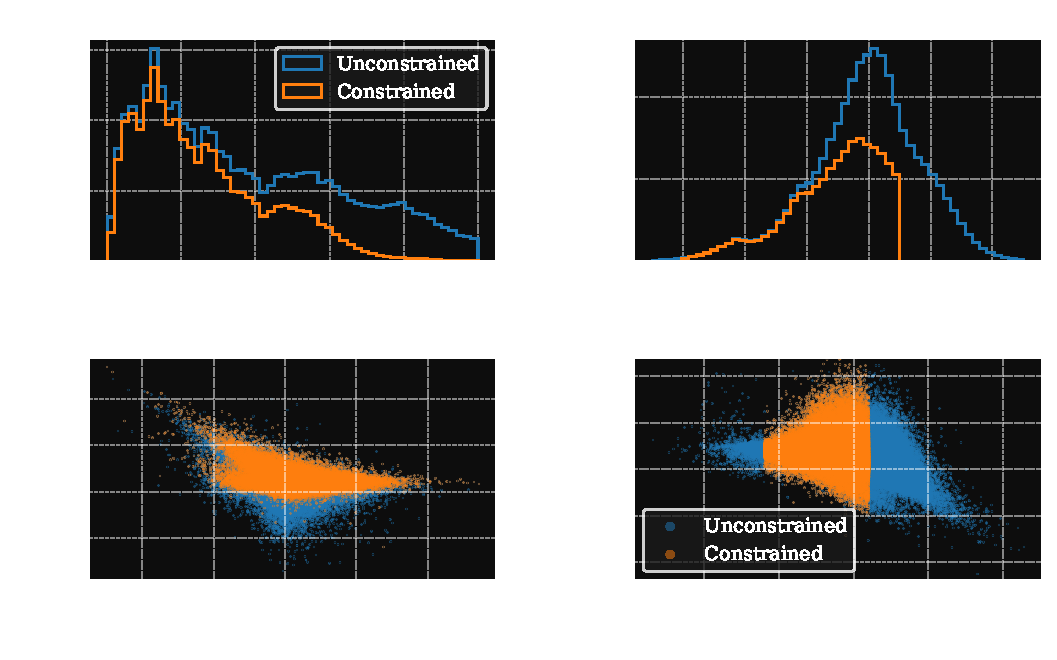
\includegraphics[height=7cm]{script/images/constraints_effect.pdf}
    \end{figure}
\end{frame}

\begin{frame}[c]{Pesos por objeto}
    A distribuição de spec-zs da amostra de treino é diferente da distribuição esperada no universo.
    \begin{equation*}
        P(y|\mathcal{D}) = \int P(y,\theta|\mathcal{D}) \text{d}\theta = \int P(y|\theta, \mathcal{D}) P(\theta|D) \text{d}\theta
    \end{equation*}
    % \hspace{0.5cm}
    \begin{splusbox}{}
        Os resultados para $y$ dependem dos dados $\mathcal{D}$, então o conjunto de treinamento pode introduzir viéses.
    \end{splusbox}
\end{frame}

\begin{frame}[c]{Pesos por objeto}
    Assumimos que a distribuição de $z_\text{spec}$ é conhecida para surveys limitados por fluxo, e modelamos esta distribuição como função da magnitude usando a amostra do COSMOS2020 (Weaver et al., 2022) e uma função Weibull de dois parâmetros $l$ e $k$.

    \begin{figure}
        \centering
        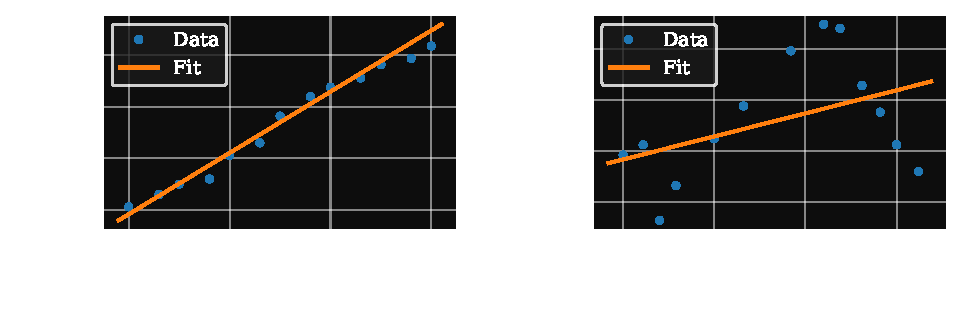
\includegraphics[width=\linewidth]{script/images/laerte_fit.pdf}
    \end{figure}
\end{frame}

\begin{frame}[c]{Pesos por objeto}
    \begin{figure}
        \centering
        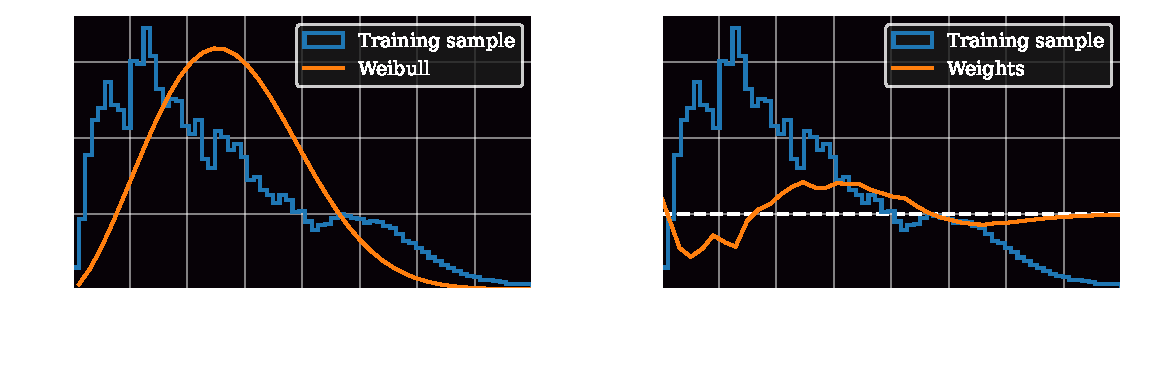
\includegraphics[width=\linewidth]{script/images/weights_vs_specz.pdf}
    \end{figure}

    Com essa abordagem, cada objeto contribui de forma diferente no treinamento do modelo
\end{frame}

\section{Metodologia}
    % \begin{tikzpicture}[overlay, remember picture]
    %     % Image 1 at specified position
    %     \node at (3.75, 1.5) {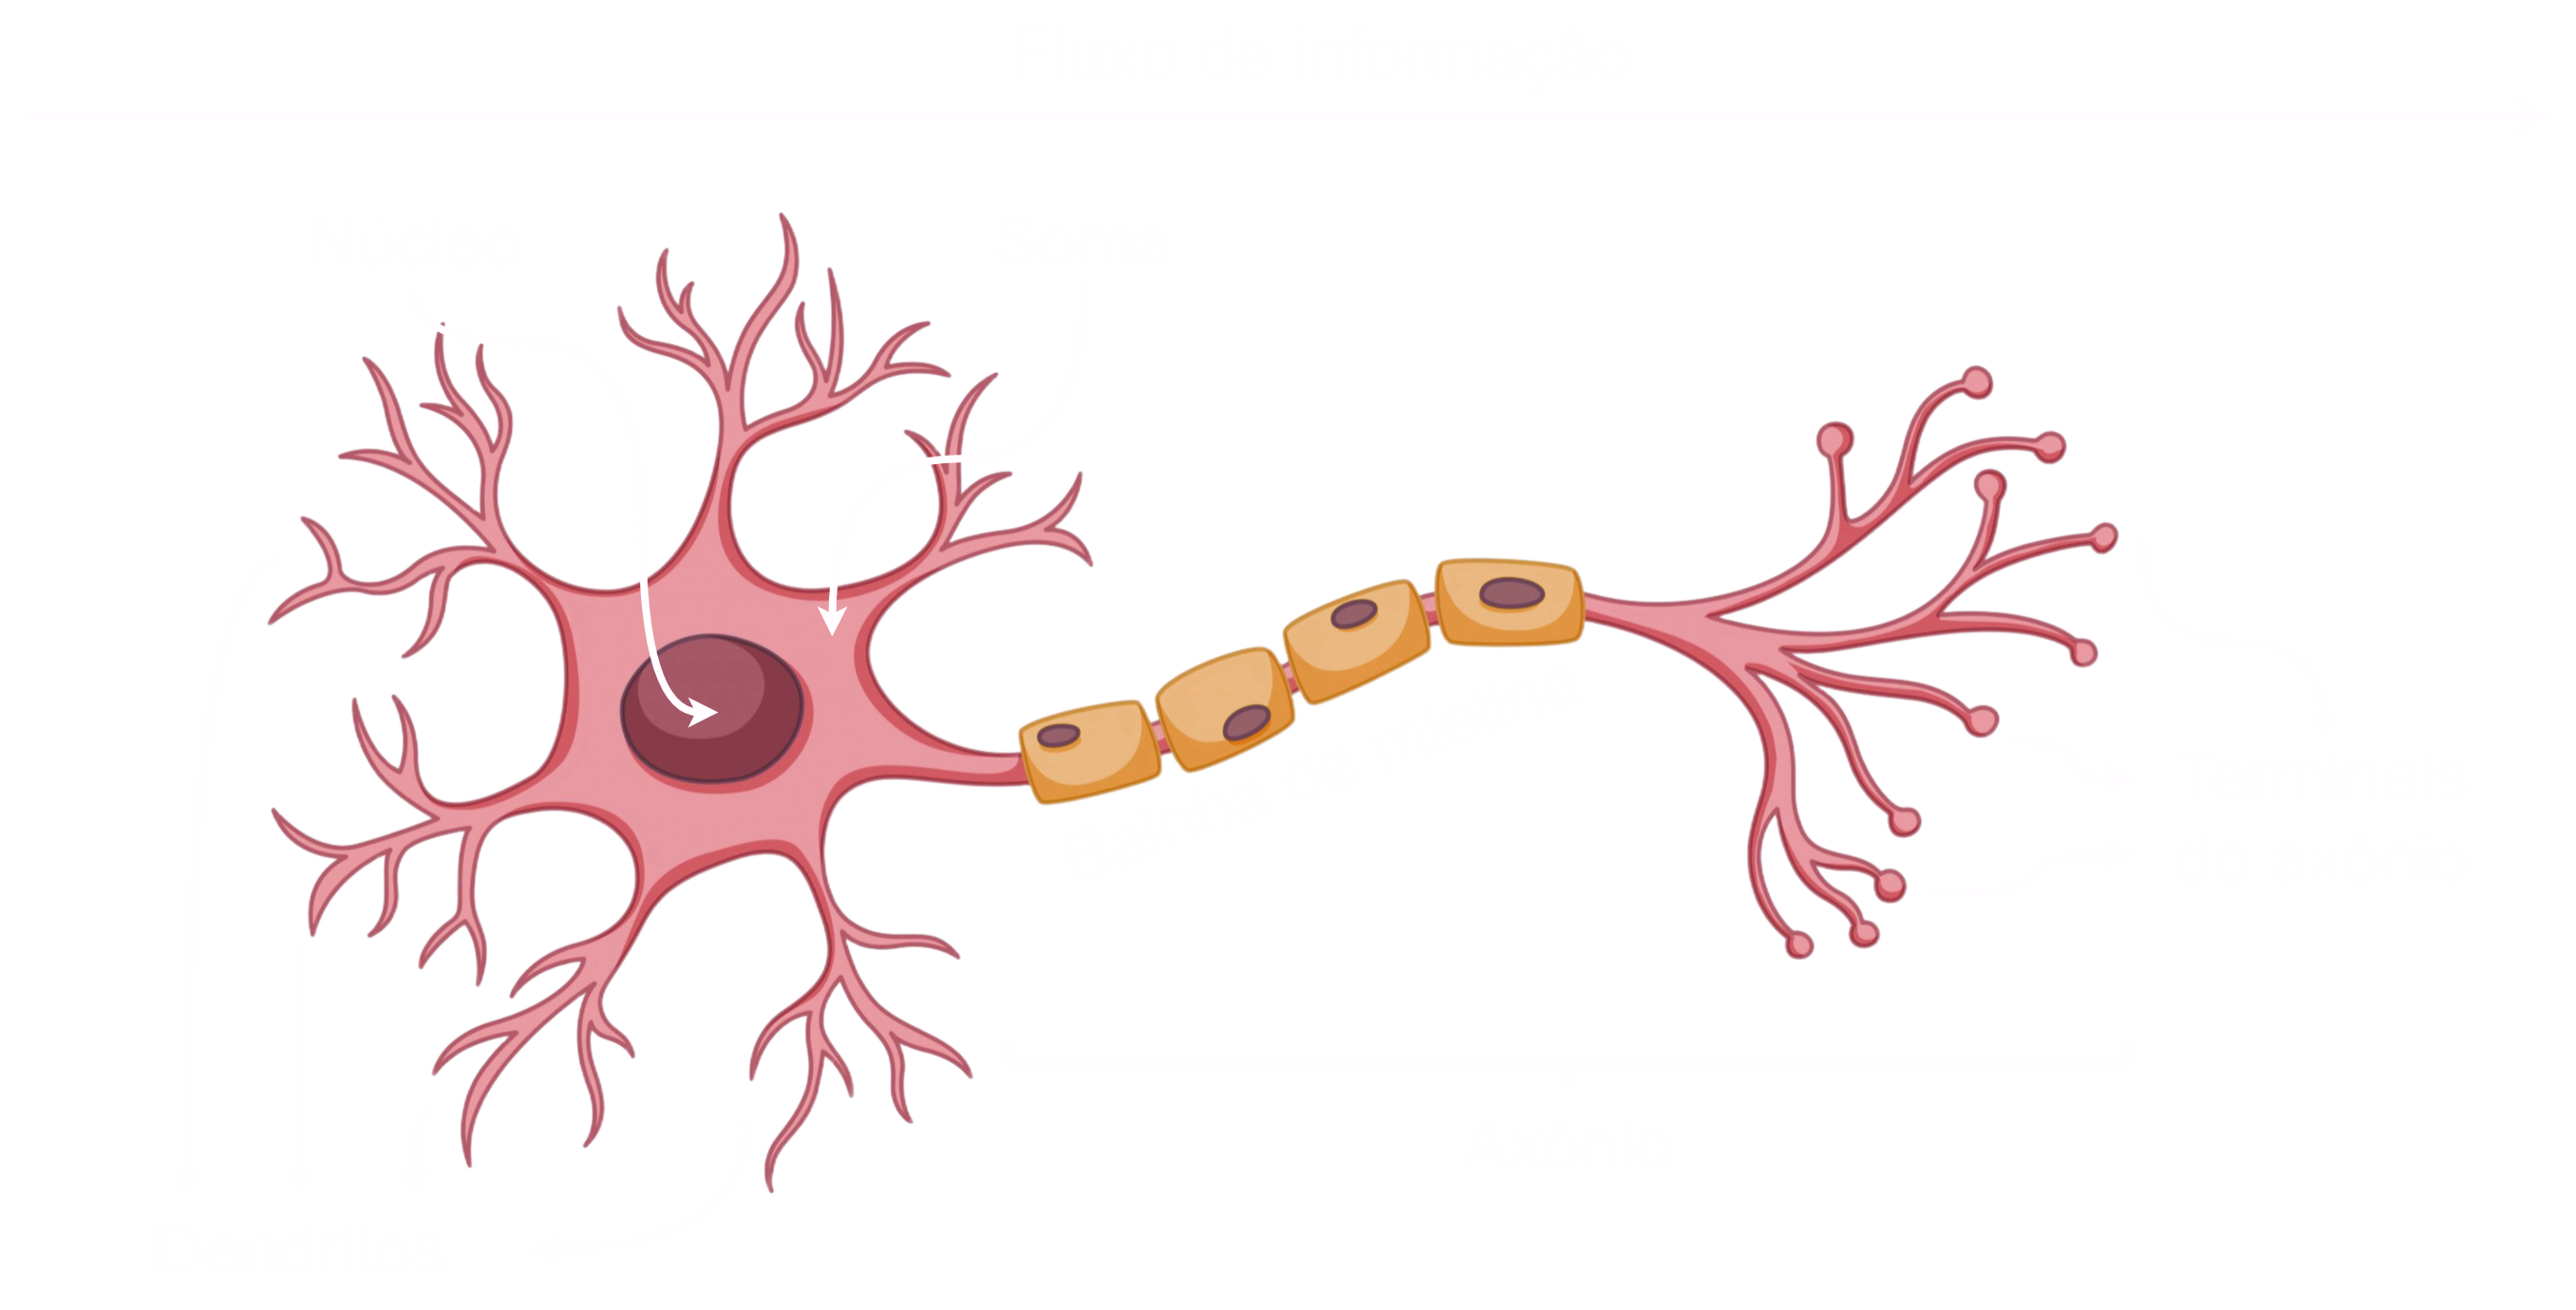
\includegraphics[height=4cm]{script/images/neuron_bio.png}};
        
    %     % Image 2 at specified position
    %     \node at (11, -1.5) {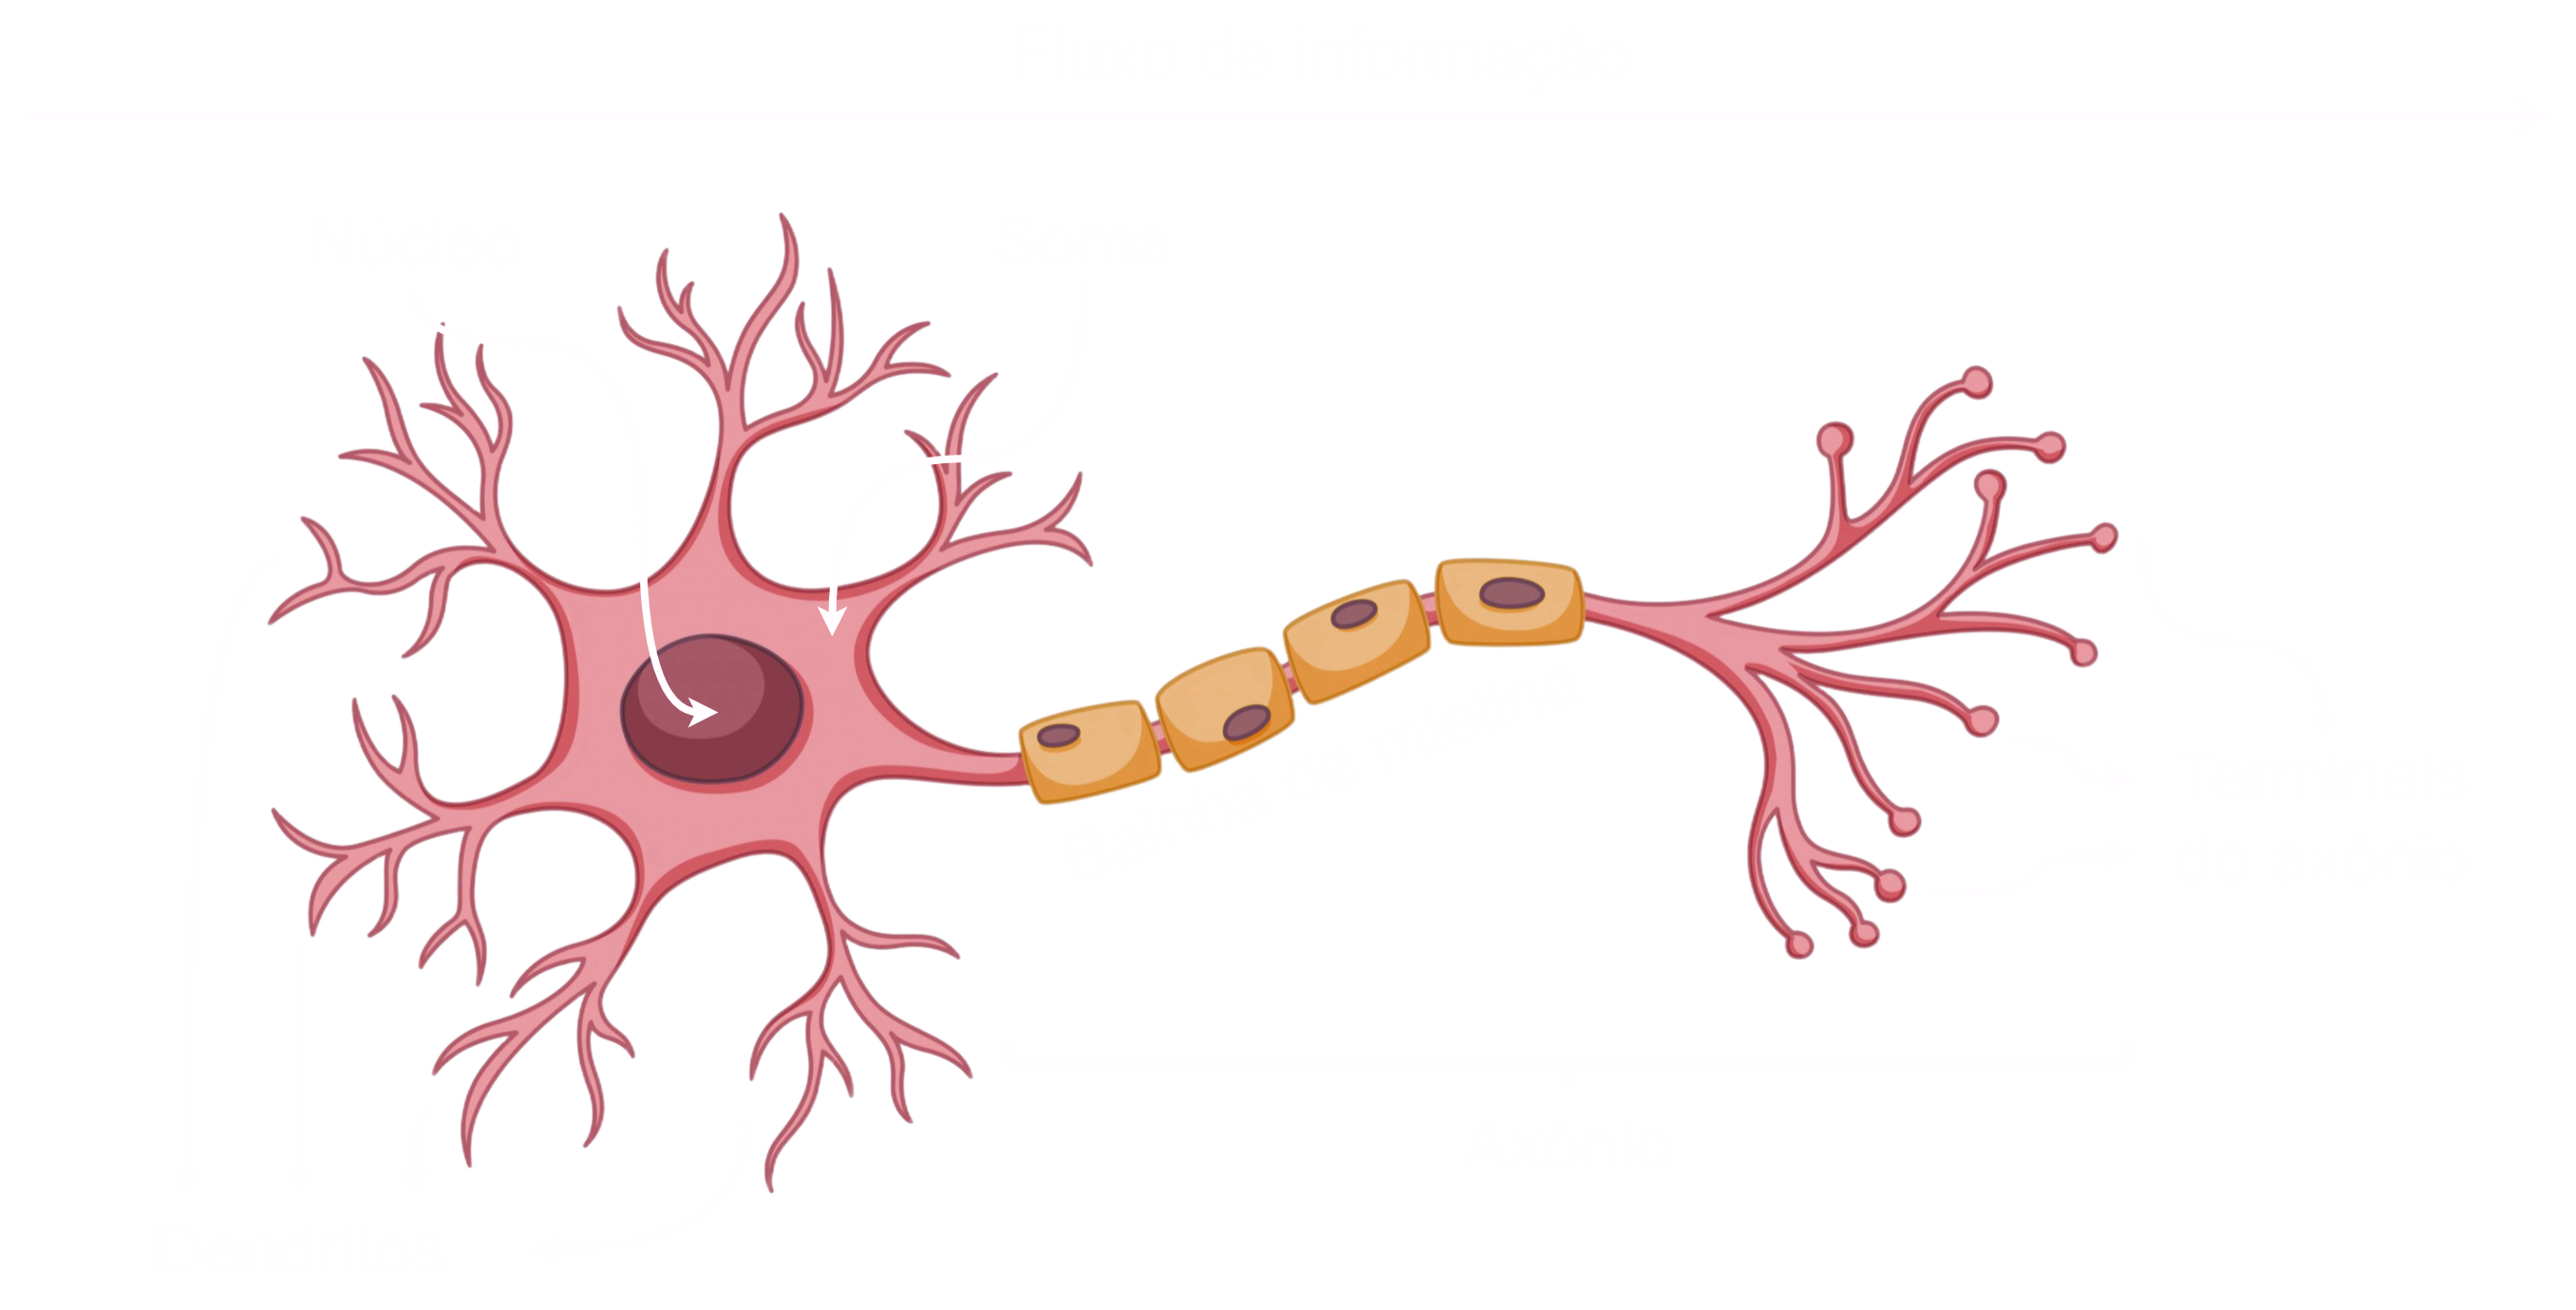
\includegraphics[height=4cm]{script/images/neuron_bio.png}};
    % \end{tikzpicture}

\begin{frame}[c]{Redes neurais}
    \begin{figure}
        \centering
        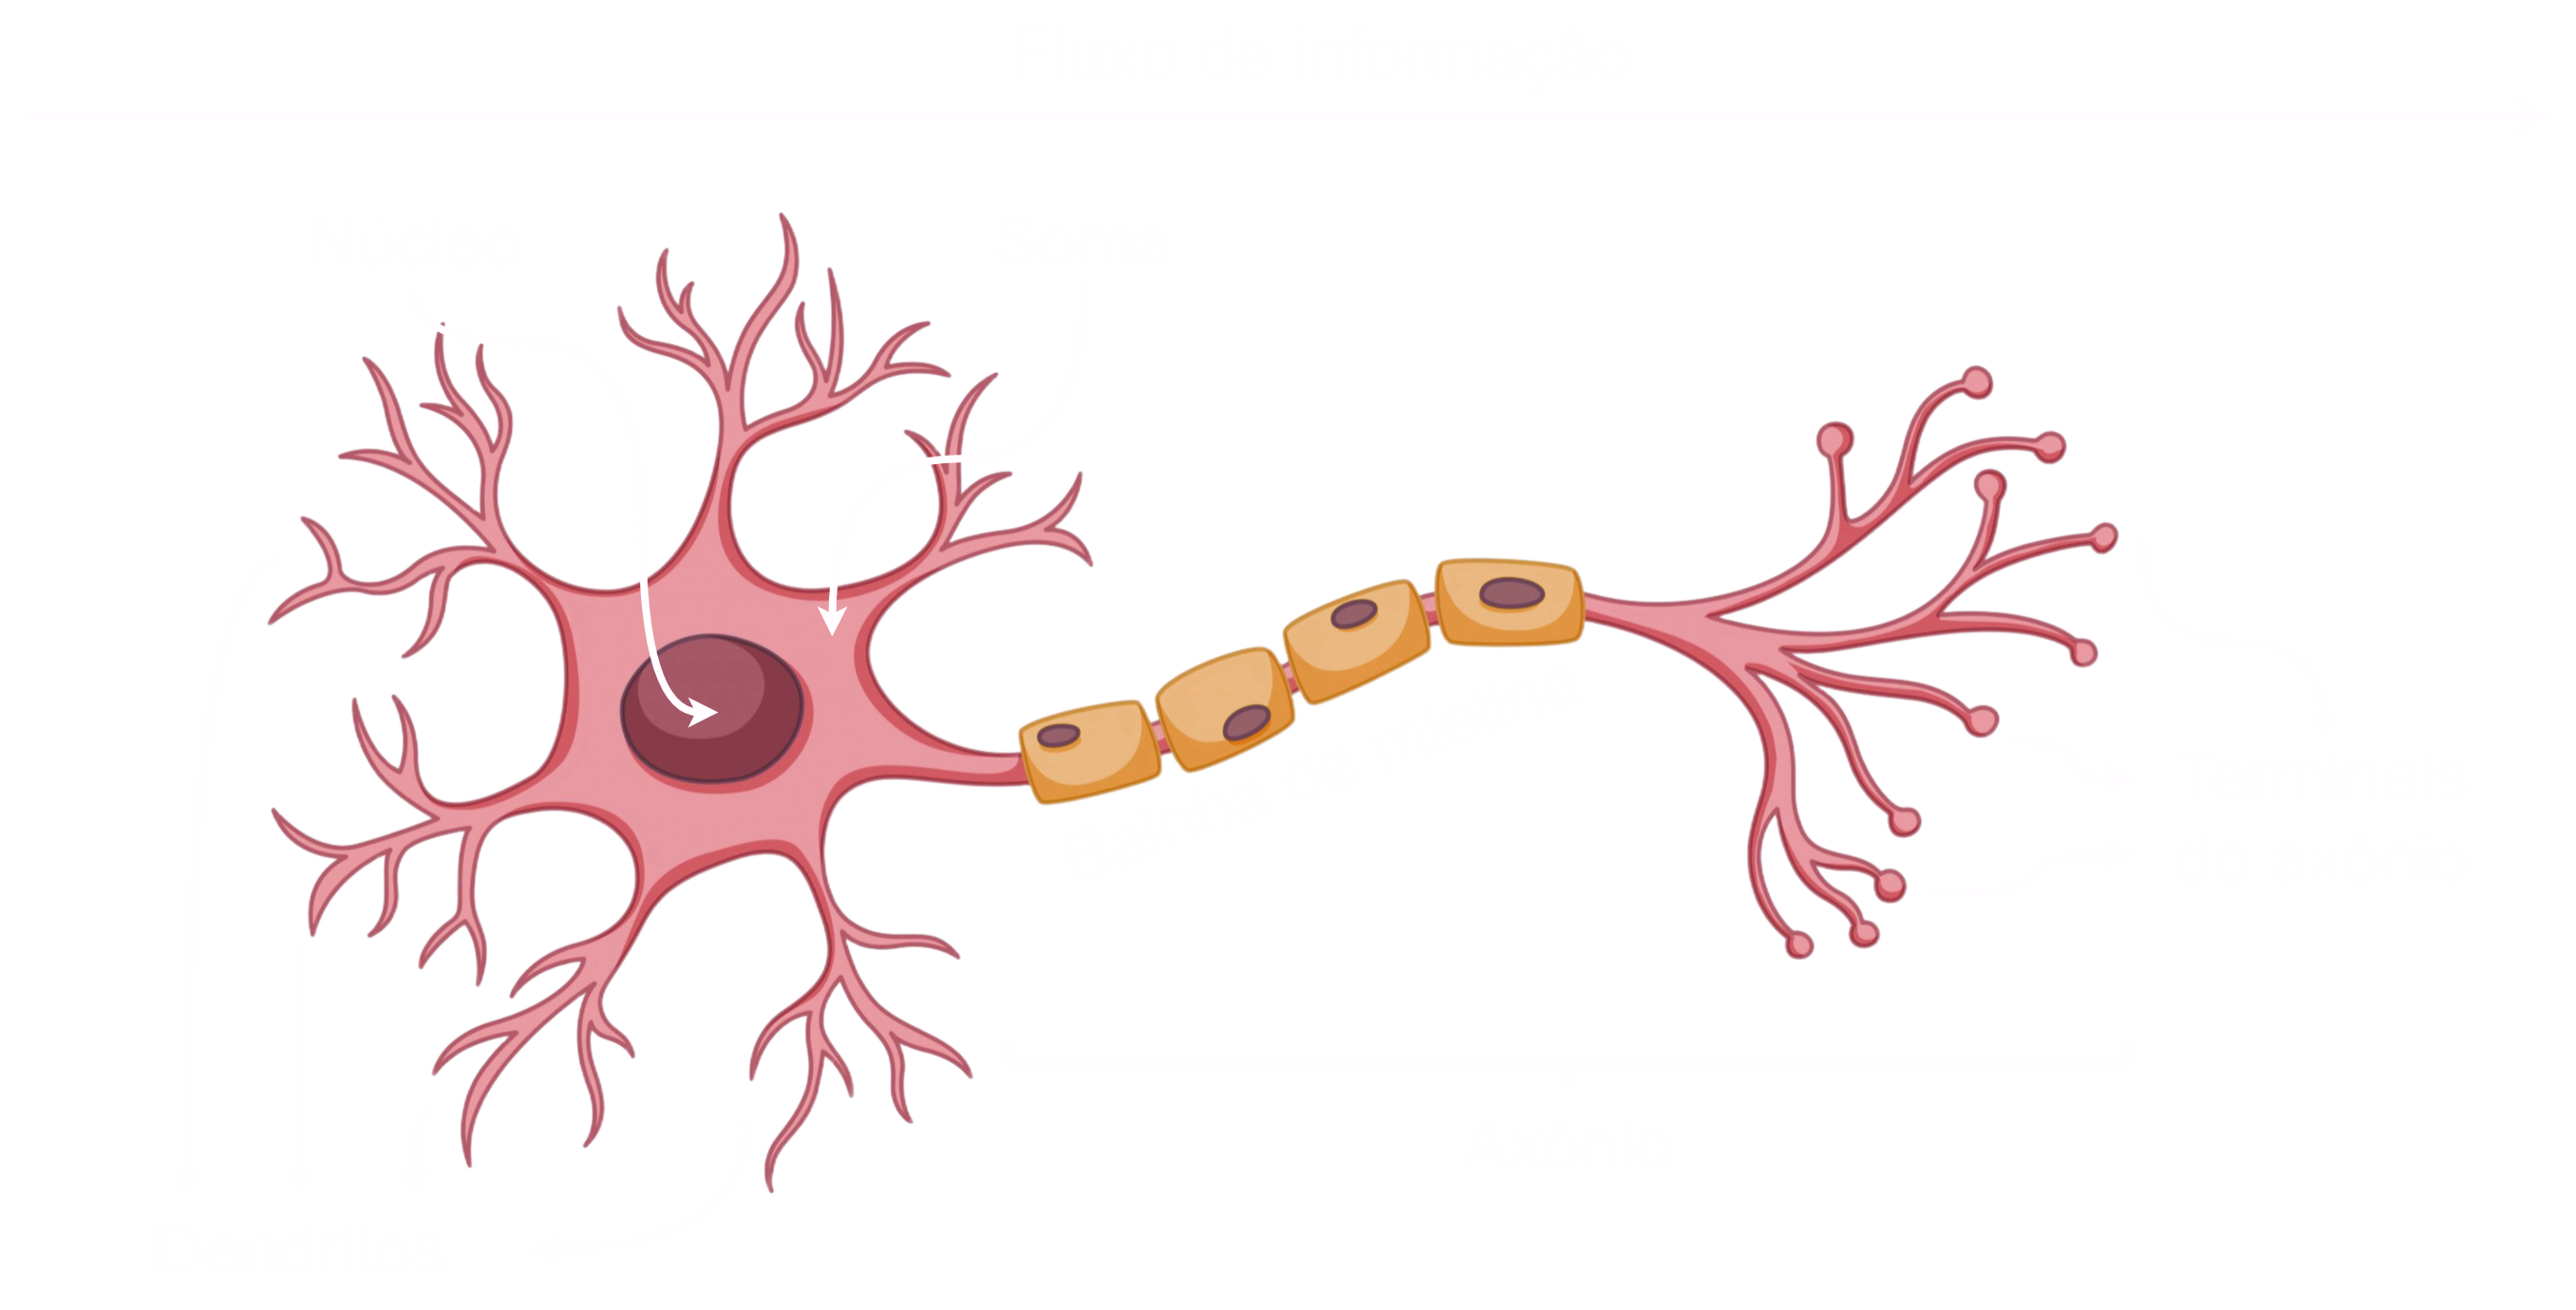
\includegraphics[height=6cm]{script/images/neuron_bio.png}
    \end{figure}
\end{frame}

\begin{frame}[c]{Redes neurais}
    \begin{figure}
        \centering
        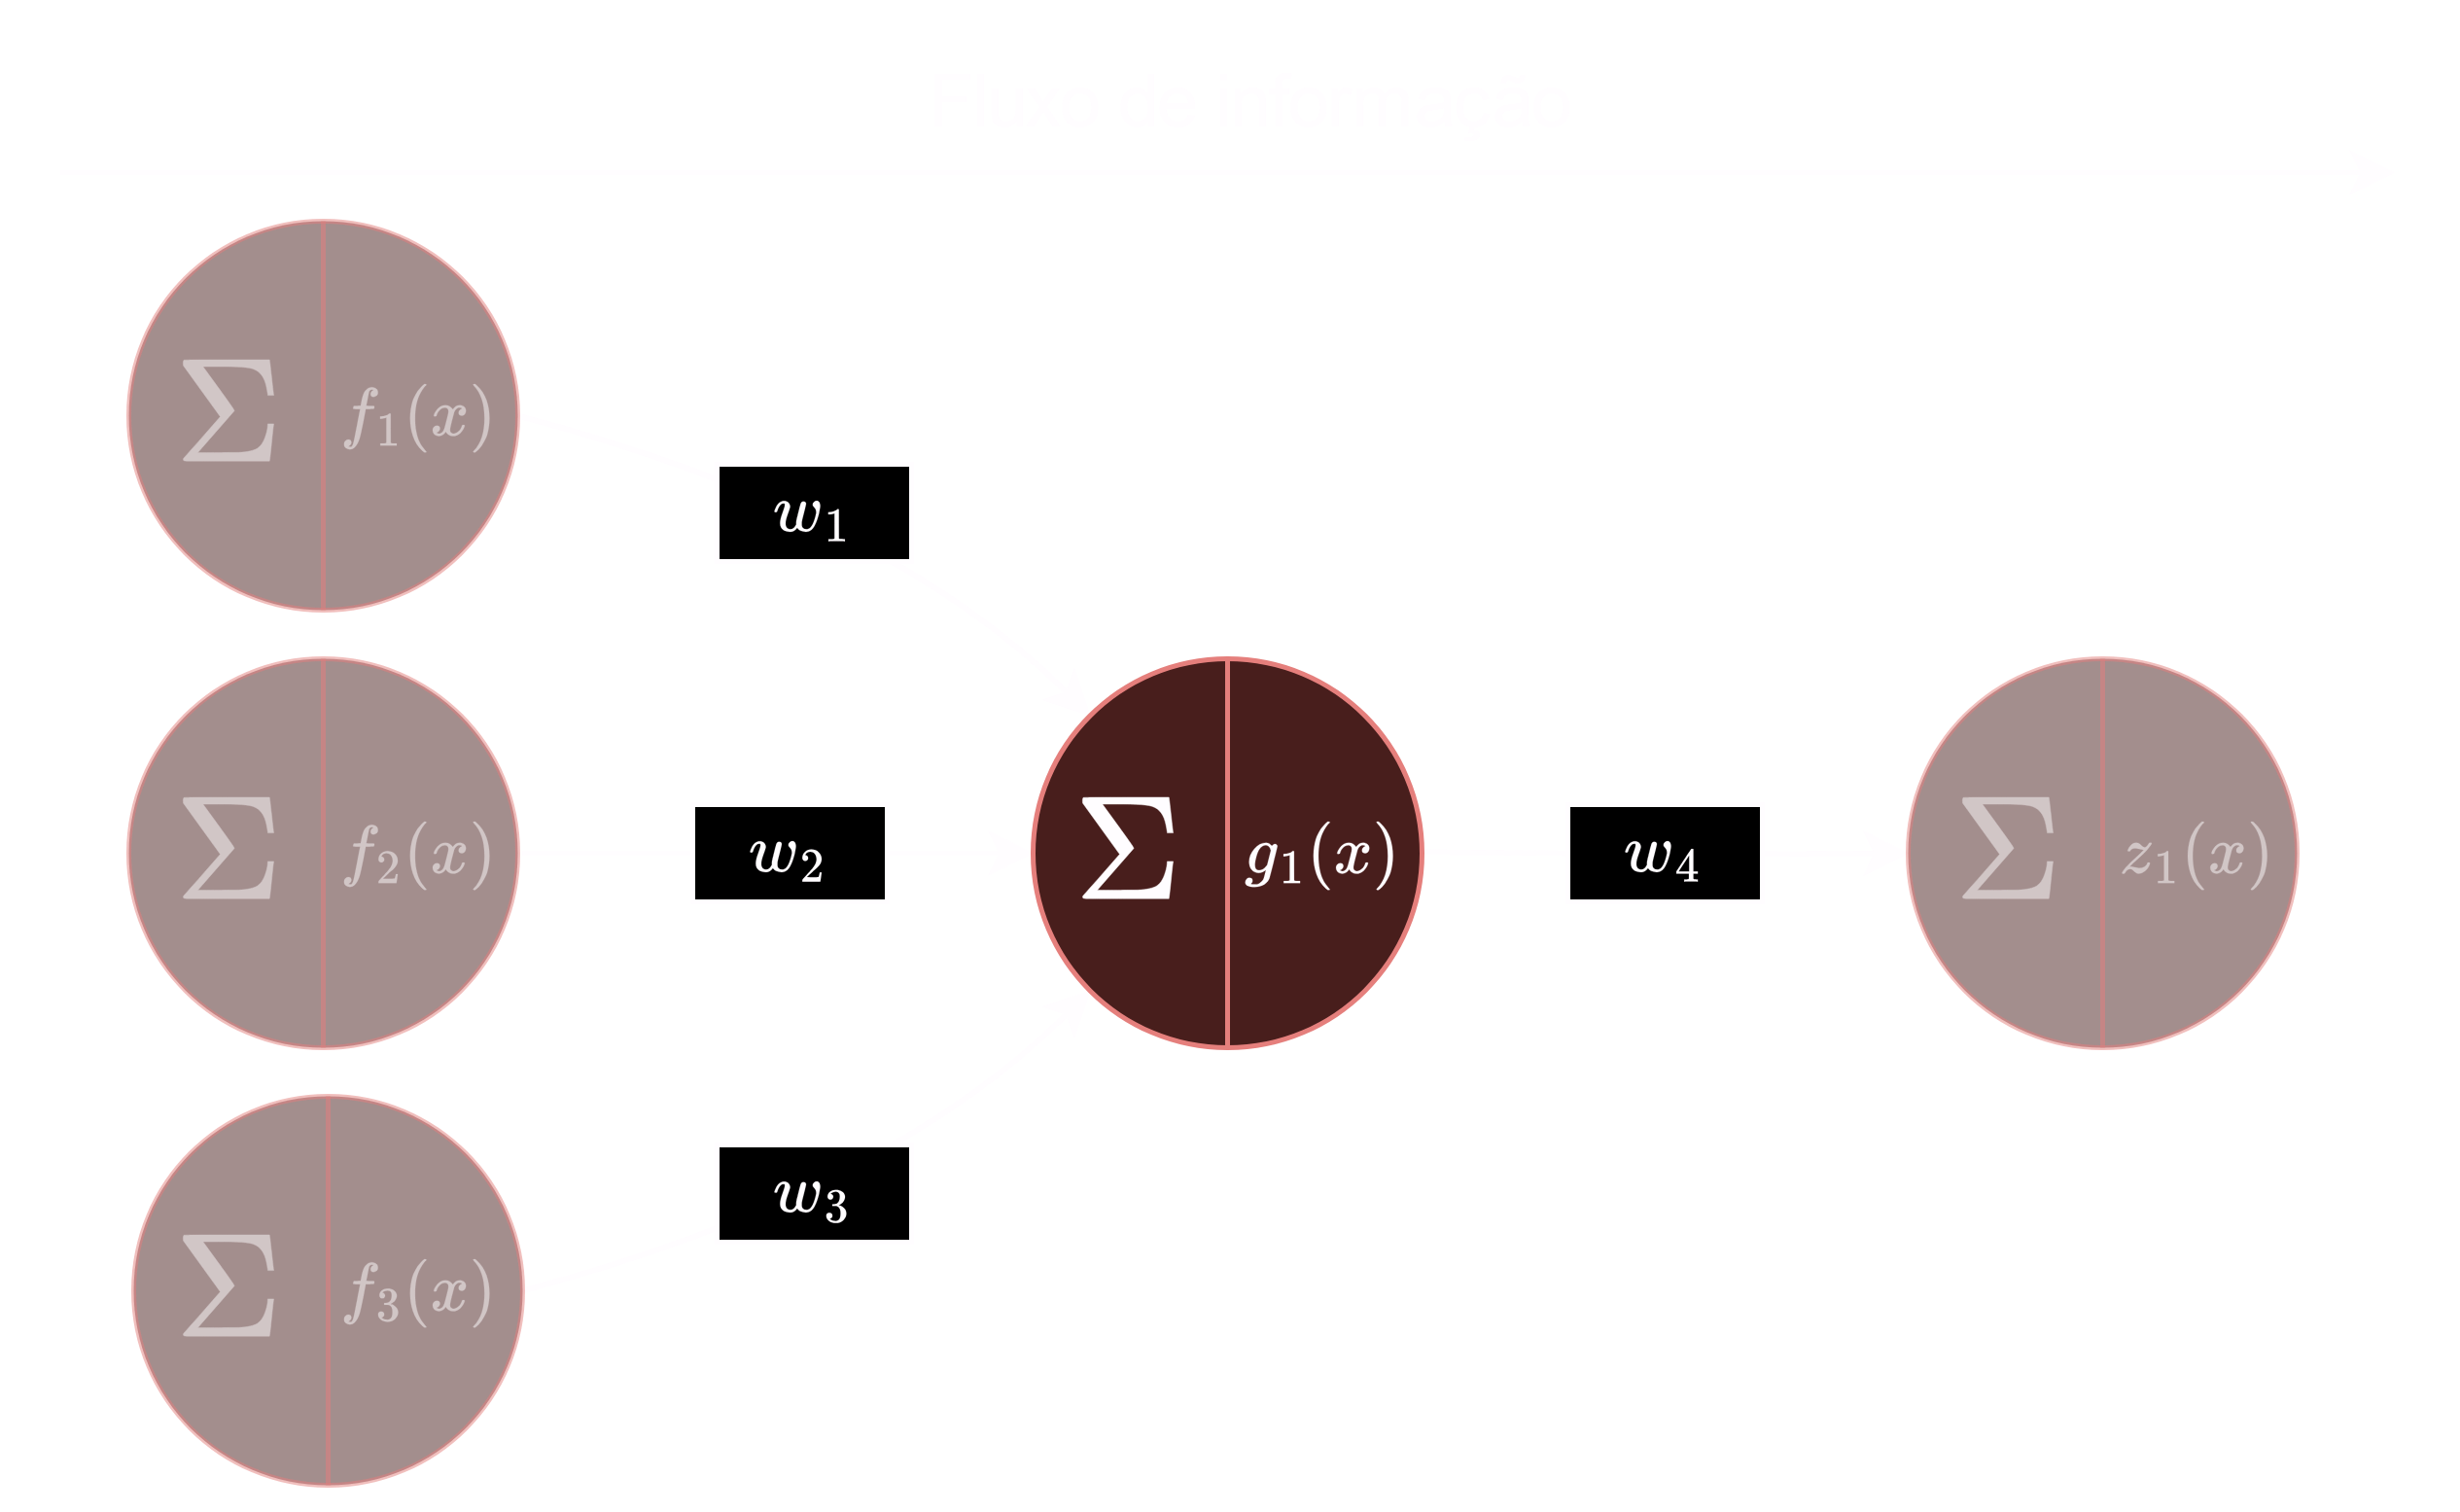
\includegraphics[height=6cm]{script/images/neuron_ml_pesos.png}
    \end{figure}
\end{frame}

% \begin{frame}[c]{Redes neurais}
%     \begin{figure}
%         \centering
%         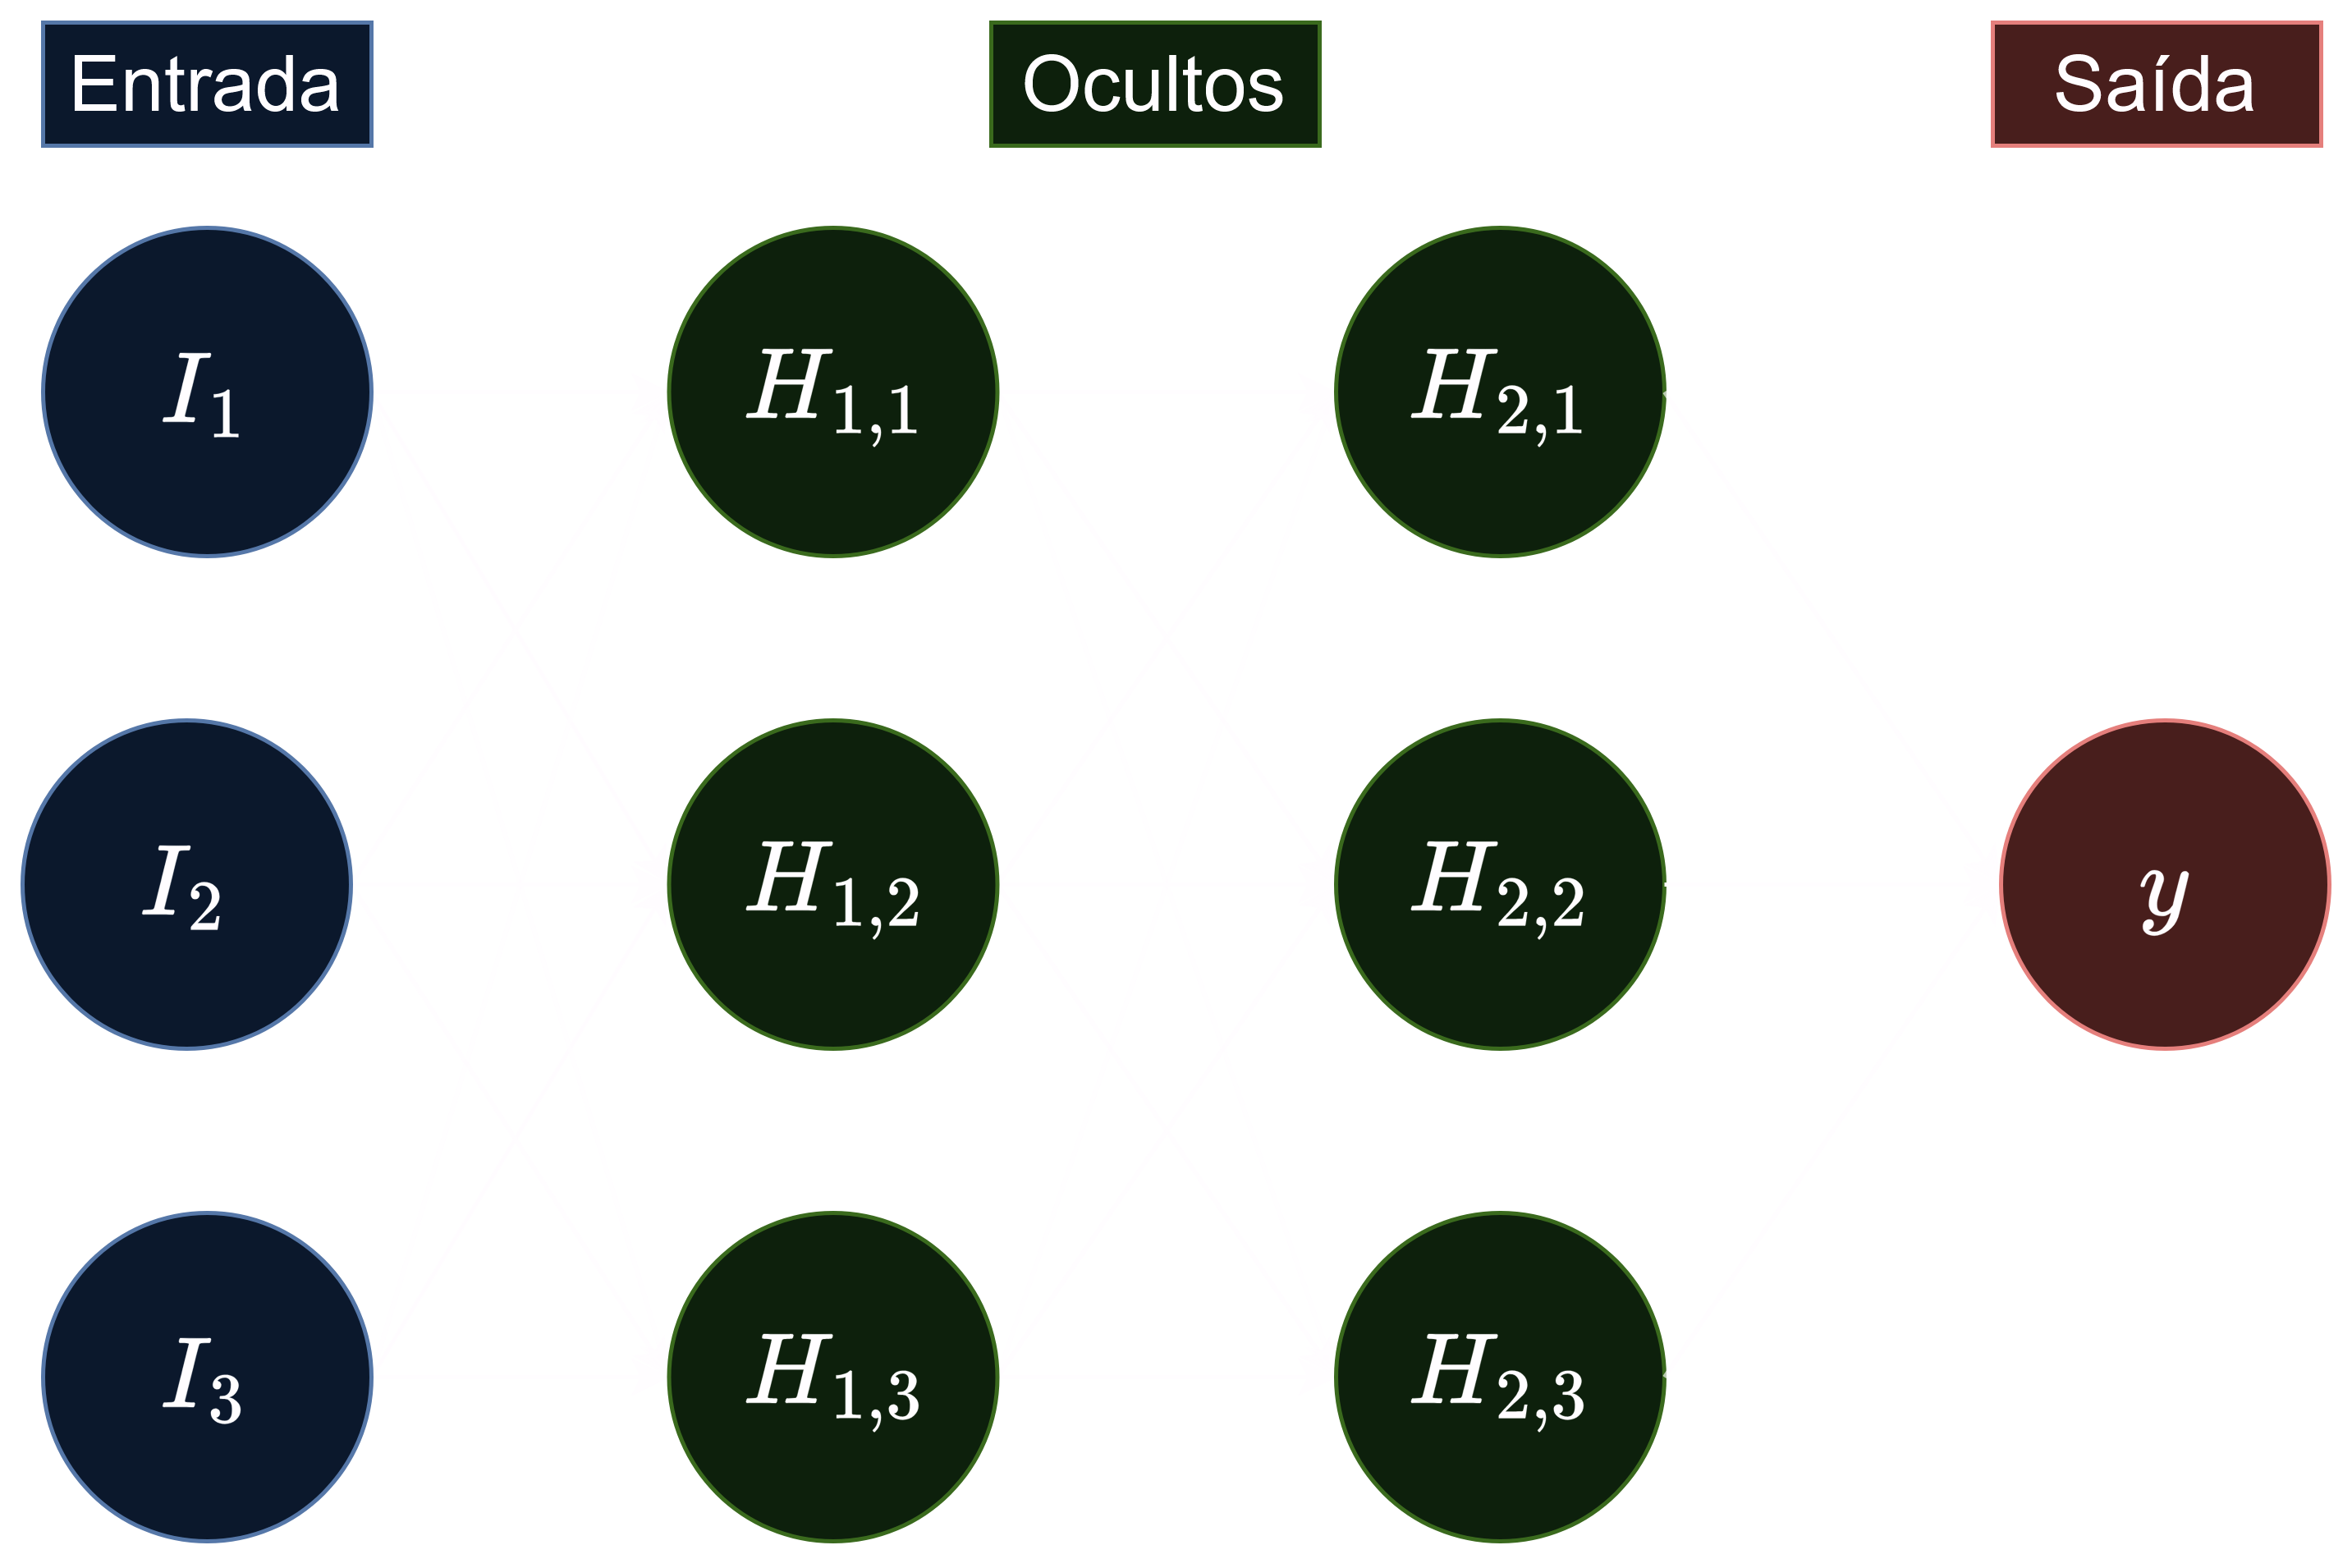
\includegraphics[height=6cm]{script/images/rede_normal.png}
%     \end{figure}
% \end{frame}

\begin{frame}[c]{Redes neurais Bayesianas}
    \begin{figure}
        \centering
        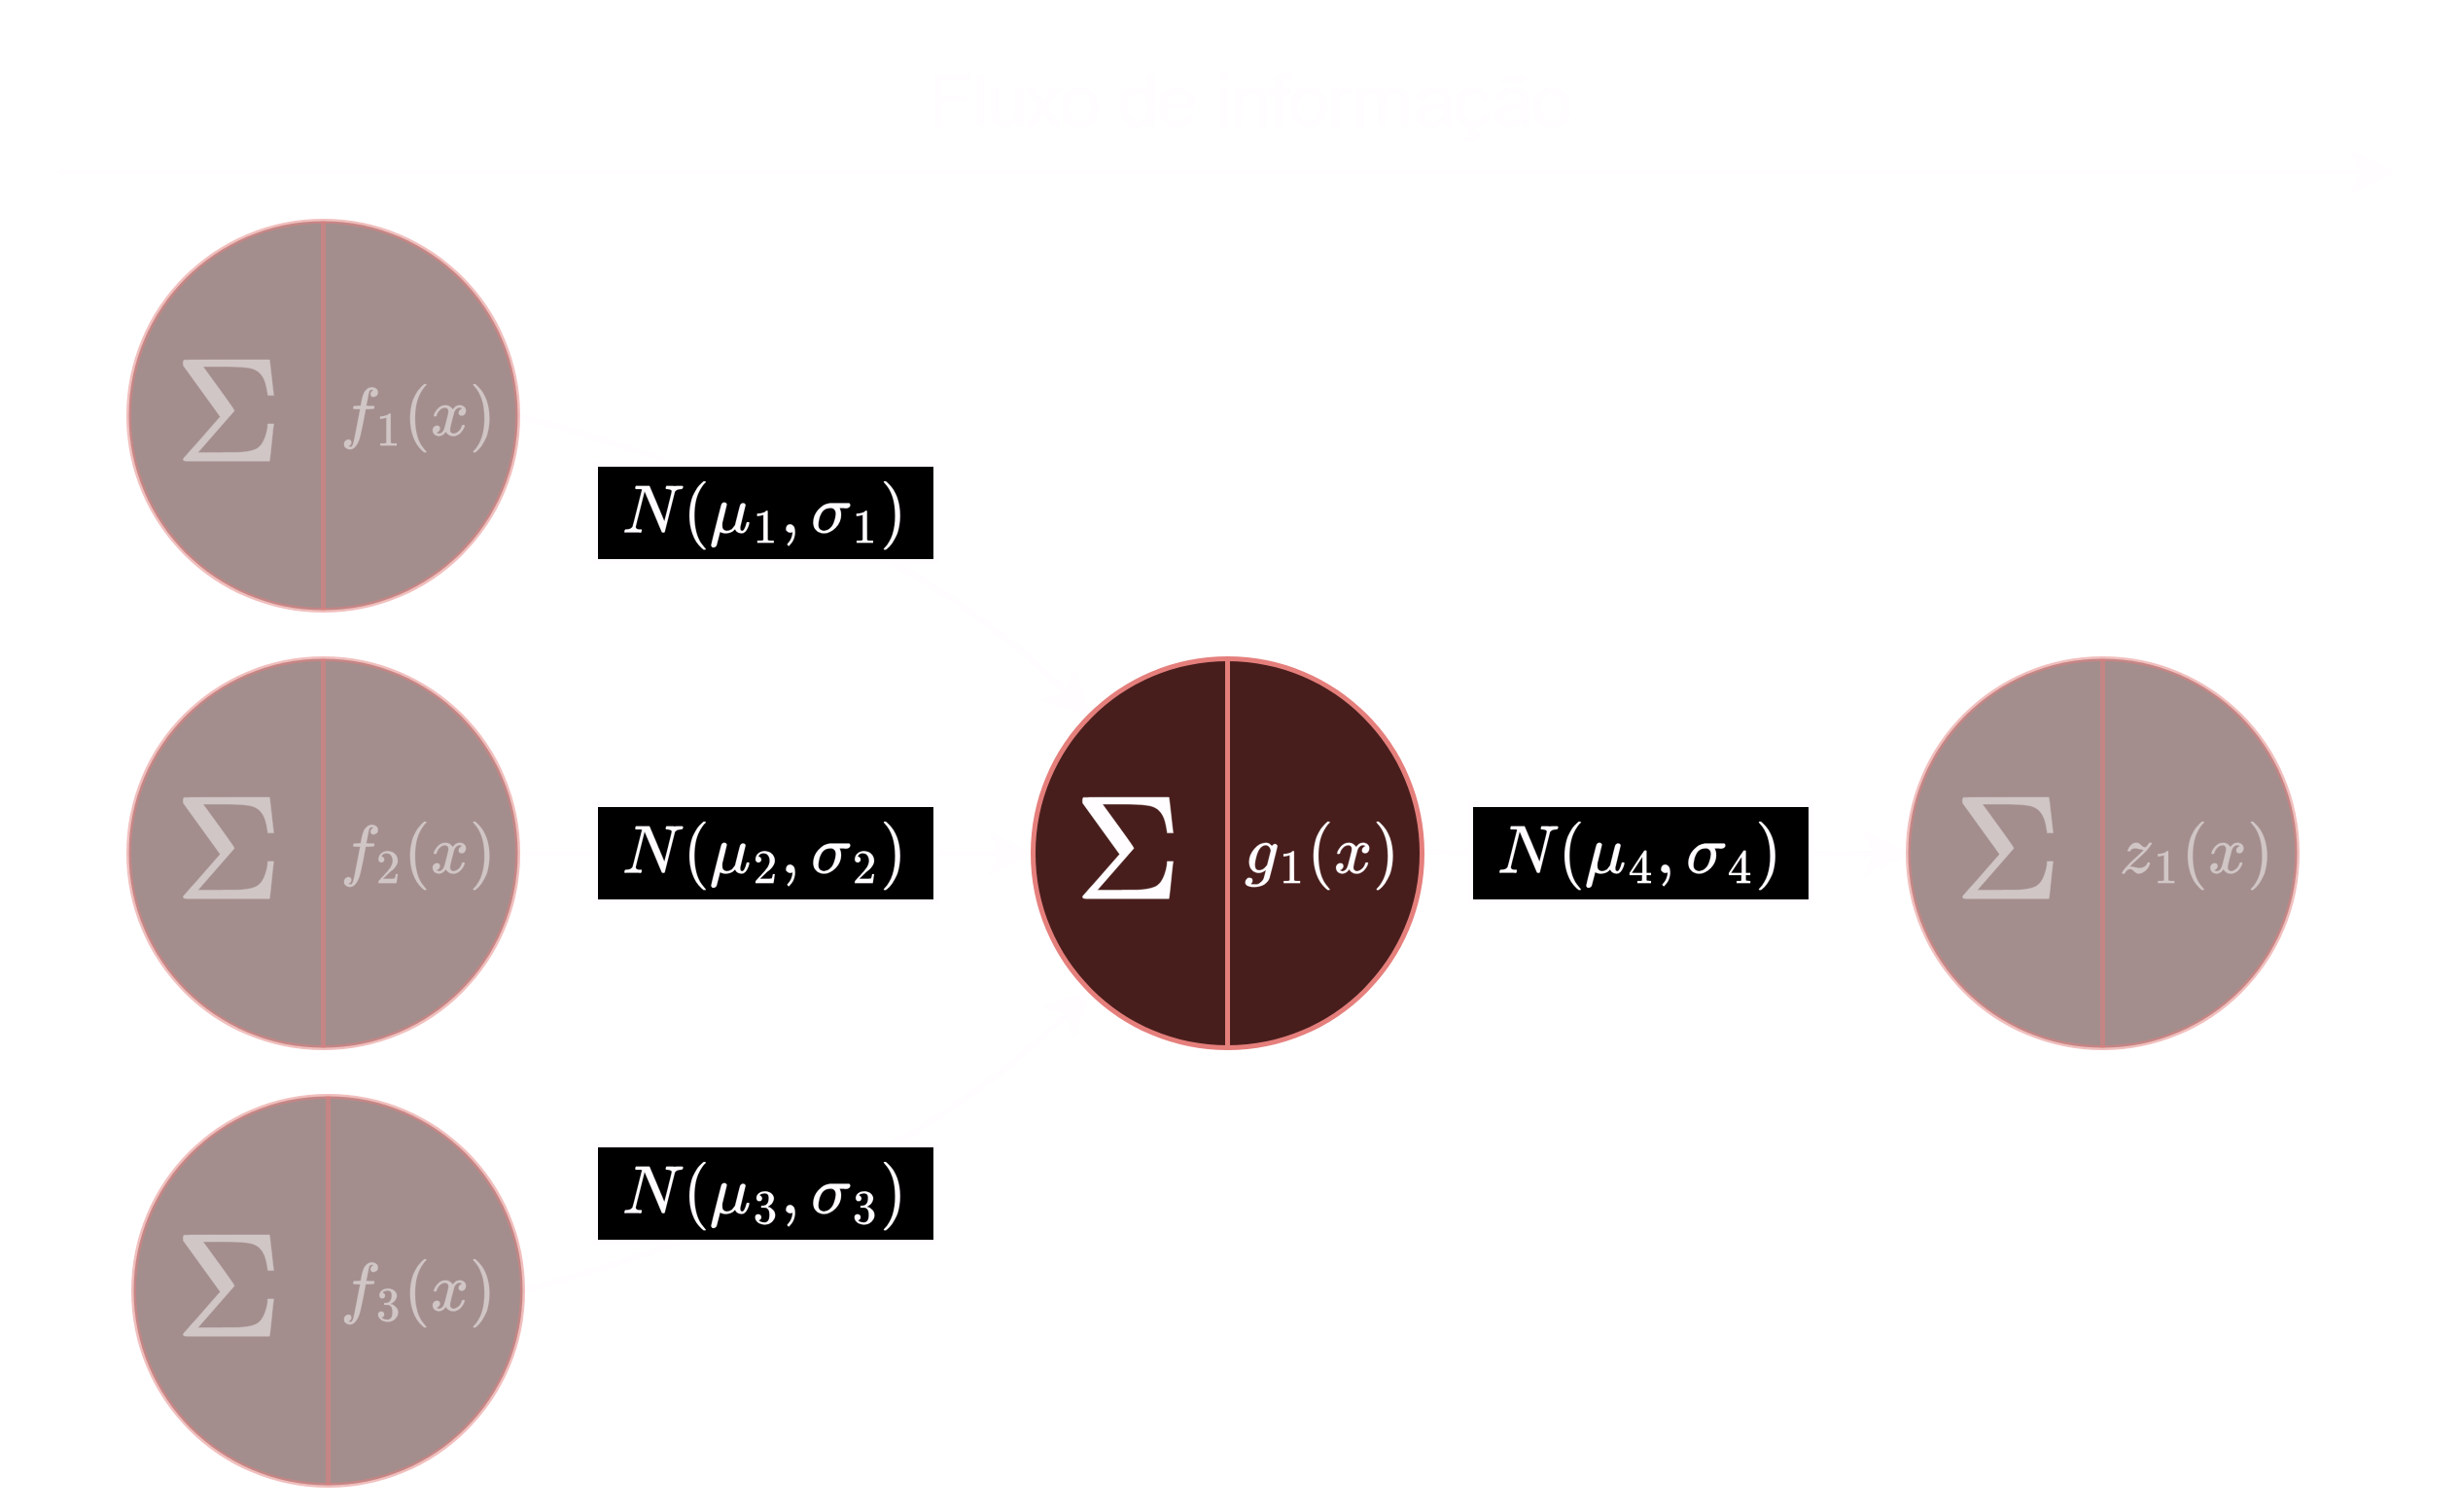
\includegraphics[height=6cm]{script/images/neuron_ml_bayes.png}
    \end{figure}
\end{frame}

\begin{frame}[c]{Redes de mistura de densidades}
    \begin{figure}
        \centering
        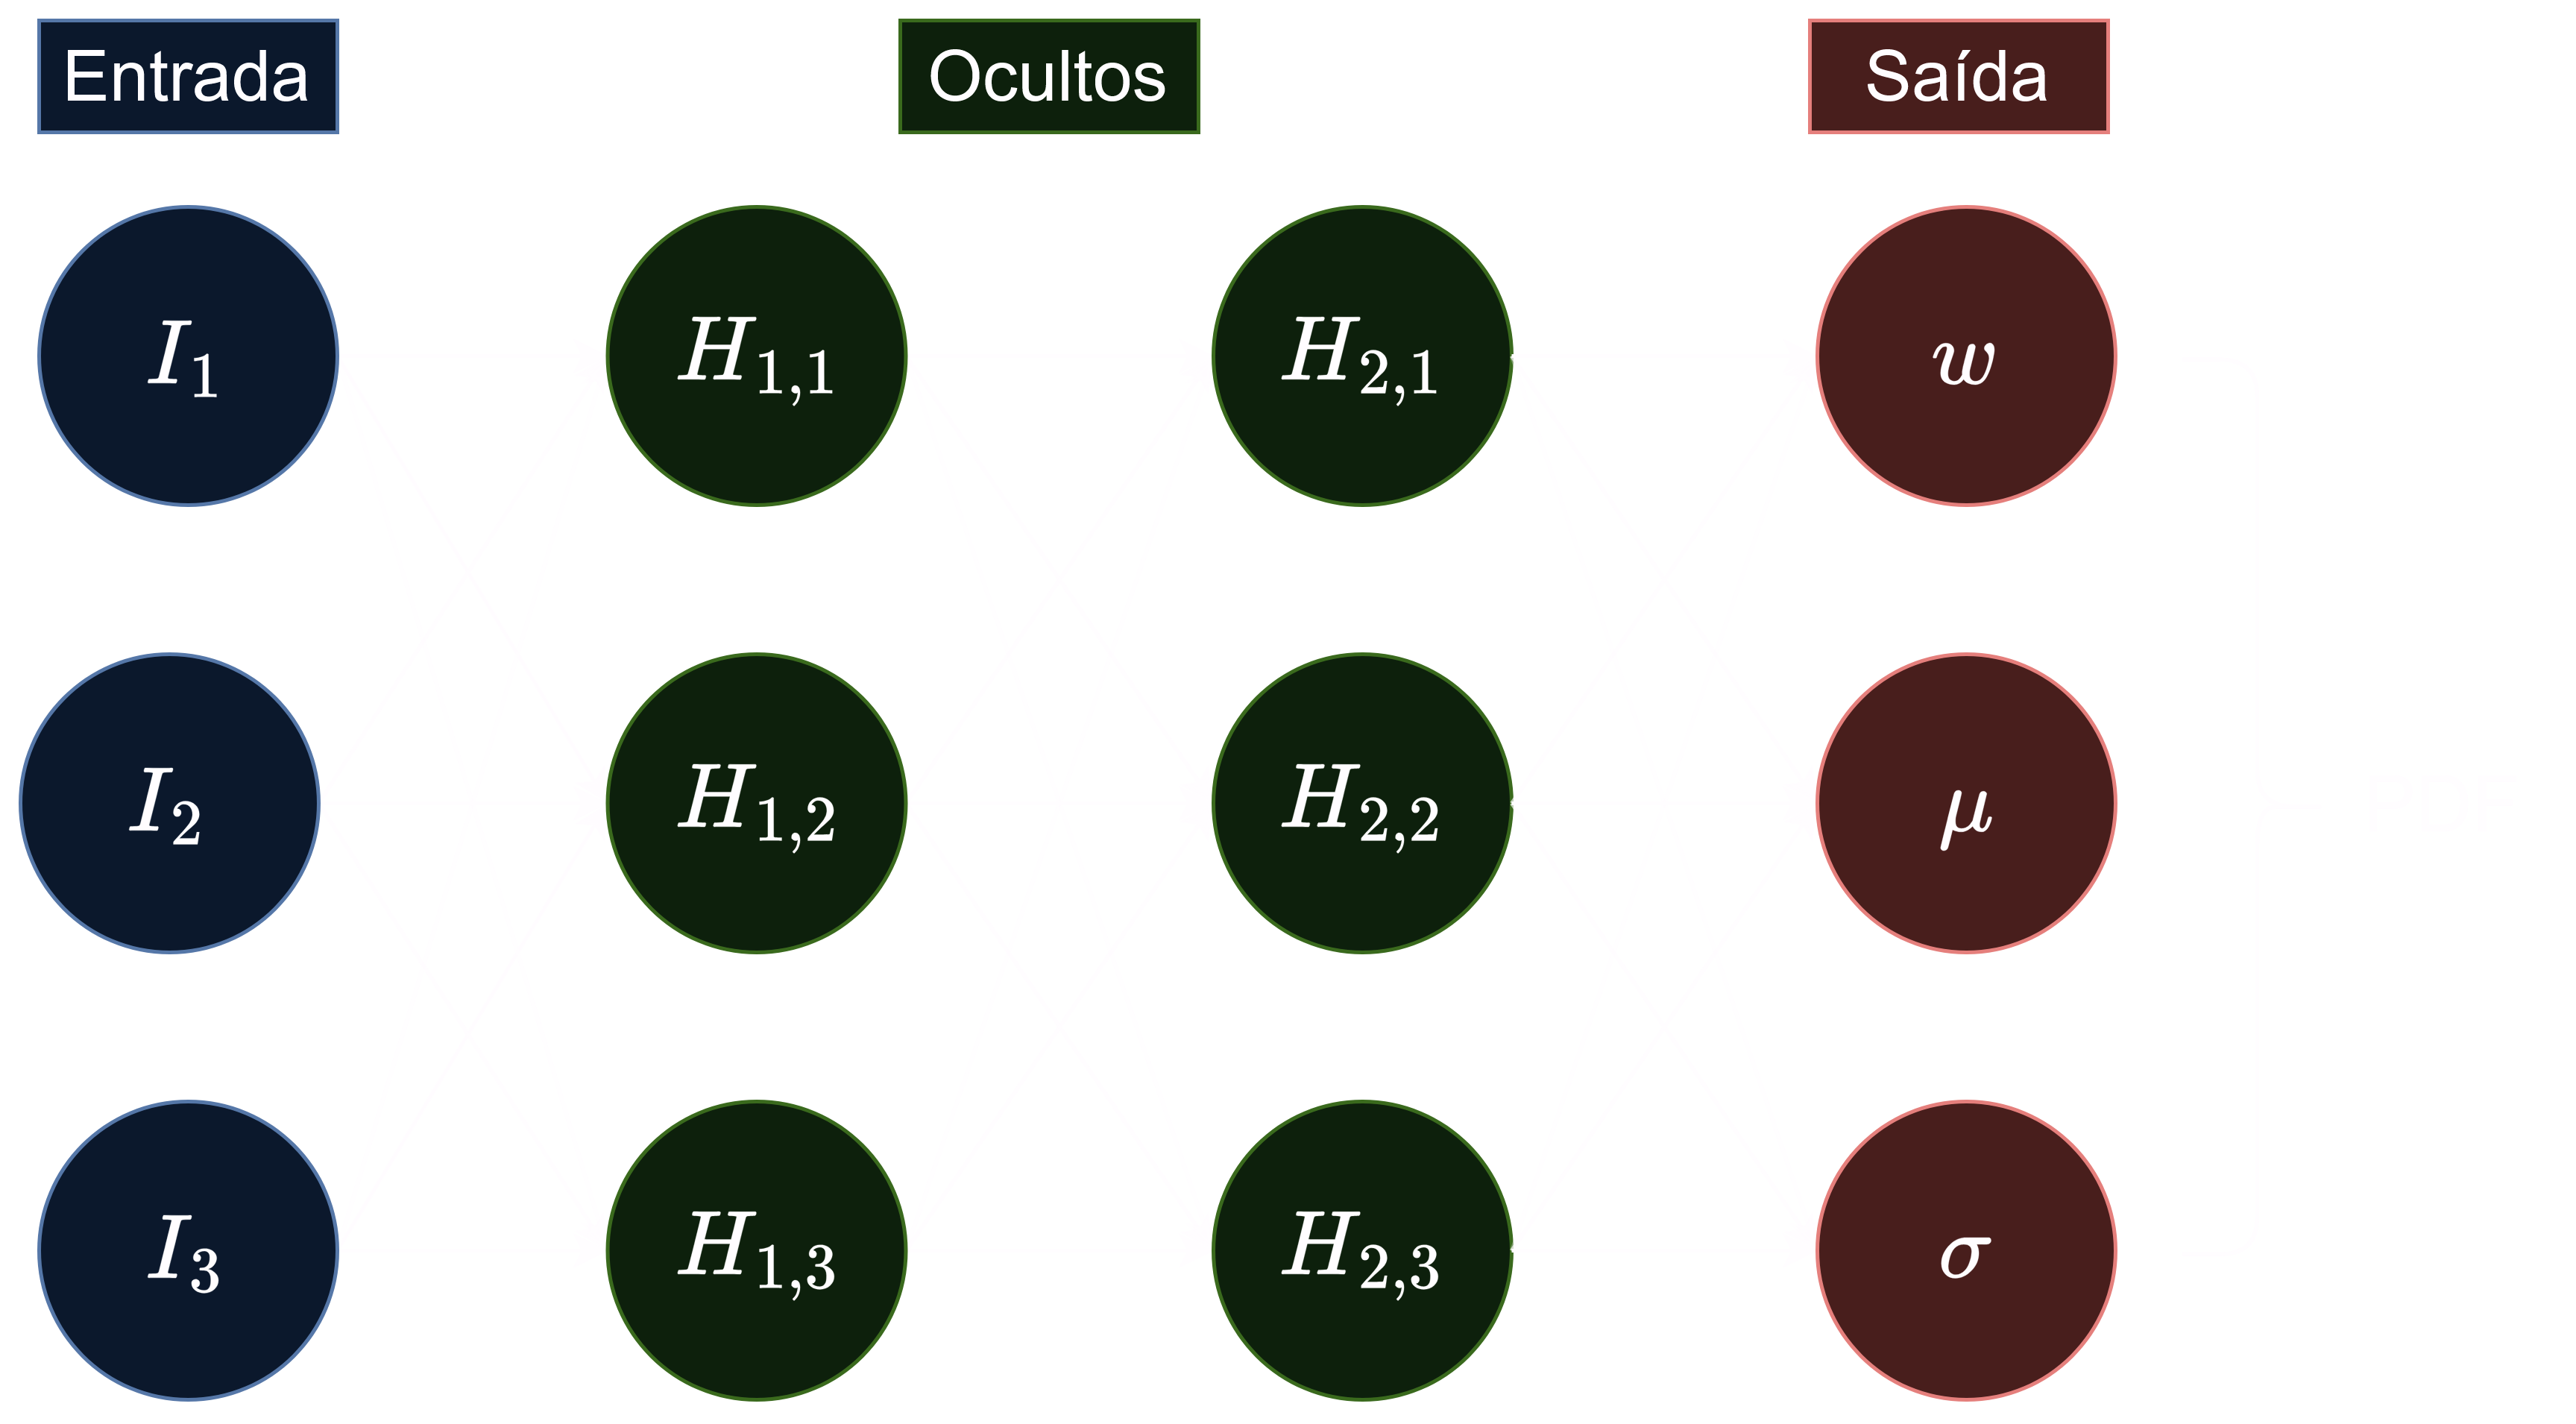
\includegraphics[height=6cm]{script/images/rede_mdn.png}
    \end{figure}
\end{frame}

\begin{frame}[c]{Redes de mistura de densidades}
    \begin{figure}
        \centering
        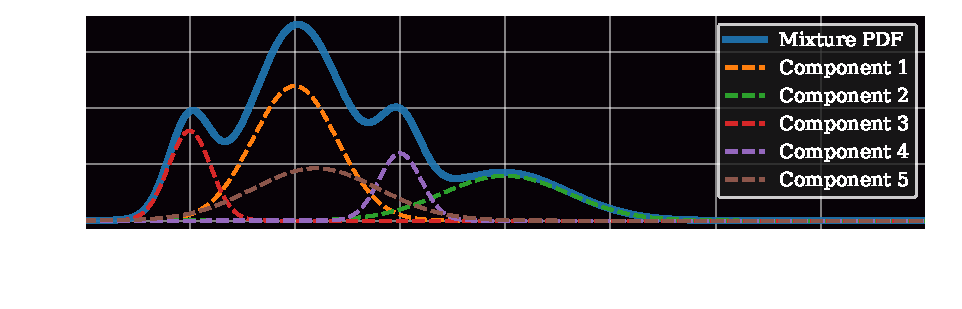
\includegraphics[width=\linewidth]{script/images/mixture_pdf_5comp.pdf}
    \end{figure}
\end{frame}

\begin{frame}[c]{Redes de mistura de densidades Bayesiana}
    Usamos uma combinação da abordagem Bayesiana com a de mistura de densidades, criando uma rede cujos pesos são distribuições e que, como saida, fornece $N$ componentes de uma mistura de densidades.

    \begin{columns}[c]
        \begin{column}{0.46\textwidth}
            \begin{splusbox}{Bayesian Neural Network}
                \begin{itemize}
                    \item Modelagem de incertezas
                    \begin{itemize}
                        \item Aleatória (dos dados)
                        \item Epistêmica (do modelo)
                    \end{itemize}
                \end{itemize}
            \end{splusbox}
        \end{column}
        \begin{column}{0.46\textwidth}
            \begin{splusbox}{Mixture Density Network}
                \begin{itemize}
                    \item Gera PDFs bem calibradas diretamente, inteiramente descritas por poucos parâmetros
                    \item É eficiente em termos de armazenamento
                \end{itemize}
            \end{splusbox}
        \end{column}
    \end{columns}

    % \begin{itemize}
    %     \justifying
    %     \item A abordagem Bayesiana permite que a rede leve em conta incertezas inerentes do problema, como aquelas devido à medição da fotometria (aleatória) e das estimativas do modelo (epistêmica).
    %     \item É capaz de produzir funções de densidade de probabilidade (PDFs) de forma natural e direta, sendo que estas são calibradas durante o treinamento do modelo.
    % \end{itemize}
\end{frame}

\section{Definindo a arquitetura}
\begin{frame}[c]{Definindo a arquitetura da rede com o \texttt{Optuna}}
    \begin{figure}
        \centering
        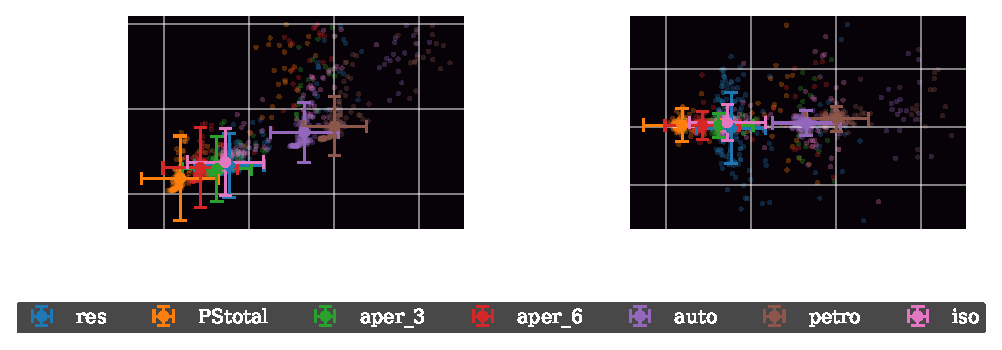
\includegraphics[width=\linewidth]{script/images/optuna_metrics_scatter.pdf}
    \end{figure}
\end{frame}

% \begin{frame}[c]{Definindo a arquitetura da rede com o \texttt{Optuna}}
%     \begin{columns}[c]
%         \small
%         \begin{column}{0.49\textwidth}
%             \begin{splusbox}{Parâmetros para amostrar}
%                 Para cada abertura do SPLUS:
%                 \begin{itemize}
%                     \item Camadas: 3 a 6
%                     \item Neurônios por camada: 64 a 128
%                     \item Função de ativação: leakyrelu, relu, elu, gelu, selu, prelu, rrelu, silu, mish, celu
%                     \item Viés nas camadas: Verdadeiro ou Falso
%                     \item Camada de atenção por feature: Verdadeiro ou falso
%                     \item Learning rate: 0.001 a 0.03
%                     \item Weight decay: 0.000001 a 0.0001
%                     \item Otimizador: adam, nadam, adamw, adabelief, ranger
%                 \end{itemize}
%             \end{splusbox}
%         \end{column}
%         \begin{column}{0.49\textwidth}
%             \begin{splusbox}{Parâmetros escolhidos}
%                 Abertura PStotal
%                 \begin{itemize}
%                     \item Camadas: 4
%                     \item Neurônios: 64
%                     \item Função de ativação: gelu
%                     \item Viés nas camadas: Verdadeiro
%                     \item Camada de atenção por feature: Verdadeiro
%                     \item Learning rate: 0.0296
%                     \item Weight decay: $7.5 \times 10^{-6}$
%                     \item Otimizador: adabelief
%                 \end{itemize}
%             \end{splusbox}
%         \end{column}
%     \end{columns}
% \end{frame}

\begin{frame}[c]{Definindo a arquitetura da rede com o \texttt{Optuna}}
    \begin{table}
        \centering
          \begin{tabular}{@{}lll@{}}
              \toprule
              \textbf{Variável}   & \textbf{Parâmetros para amostrar}     & \textbf{Parâmetros escolhidos} \\ \midrule
              Camadas             & 3 a 6                                 & 4                              \\
              Neurônios           & 64 a 128                              & 64                             \\
              Ativação            & Todas as "\texttt{LU}"                  & \texttt{gelu}                  \\
              Otimizador          & Variações de \texttt{Adam}            & \texttt{AdaBelief}             \\
              Learning rate       & 0.001 a 0.03                          & 0.0296                         \\
              Weight decay        & $1 \times 10^{-6}$ a $1 \times 10^{-4}$ & $7.5 \times 10^{-6}$           \\
              Viés das camadas    & \texttt{True} ou \texttt{False}       & \texttt{True}                  \\
              Atenção por feature & \texttt{True} ou \texttt{False}       & \texttt{True}                  \\ \bottomrule
          \end{tabular}
      \end{table}

      \begin{tcolorbox}
          Em todos os casos, os valores de entrada foram   magnitudes, cores e informações morfológicas
      \end{tcolorbox}
\end{frame}

\section{Resultados}
% \begin{frame}[c]{Redshifts fotométricos: estimativas de ponto único}
%     \begin{itemize}
%         \item $\sigma_\text{NMAD}$:
%         \begin{equation*}
%             \sigma_\text{NMAD} = 1.48 \times \text{mediana} \left( \left| \frac{{\delta z} - \text{mediana}(\delta z)}{1+z_\text{spec}} \right| \right)
%         \end{equation*}
%         \item Bias ($\mu$):
%         \begin{align*}
%             \mu &= \text{mediana} \left( \delta z \right), \\
%             \mu_\text{norm} &= \text{mediana} \left( \frac{\delta z}{1+z_{\text{spec}}} \right).
%         \end{align*}
%         \item Fração de outliers ($\eta$):
%         \begin{align*}
%             \eta &= \frac{|\delta z|}{1+z_\text{spec}} > 0.15, \\
%             \eta_{N\sigma} &= \frac{|\delta z|}{1+z_\text{spec}} > N \cdot \sigma_\text{NMAD}.
%         \end{align*}
%     \end{itemize}
% \end{frame}

\begin{frame}[c]{Redshifts fotométricos: estimativas de ponto único}
    \begin{splusbox}{Desvio médio absoluto normalizado ($\sigma_\text{NMAD}${, \textcolor{LightGray}{Brammer et al., 2008}})}
        \begin{equation*}
            \sigma_\text{NMAD} = 1.48 \times \text{mediana} \left( \left| \frac{{\delta z} - \text{mediana}(\delta z)}{1+z_\text{spec}} \right| \right)
        \end{equation*}
    \end{splusbox}

    % \begin{splusbox}{Desvio médio absoluto normalizado ($\sigma_\text{NMAD}$)}
    %     \vspace{-.5cm}
    %     \begin{columns}[c]
    %         \begin{column}{0.58\textwidth}
    %             \centering
    %             \begin{equation*}
    %                 \sigma_\text{NMAD} = 1.48 \times \text{mediana} \left( \left| \frac{{\delta z} - \text{mediana}(\delta z)}{1+z_\text{spec}} \right| \right)
    %             \end{equation*}
    %         \end{column}
    %         \begin{column}{0.38\textwidth}
    %             \centering
    %             \begin{equation*}
    %                 \delta z = z_\text{phot} - z_\text{spec}
    %             \end{equation*}
    %         \end{column}
    %     \end{columns}
    % \end{splusbox}

    \begin{splusbox}{Viés ($\mu$)}
        \vspace{-.5cm}
        \begin{columns}[c]
            \begin{column}{0.46\textwidth}
                \centering
                \begin{equation*}
                    \mu = \text{mediana} \left( \delta z \right)
                \end{equation*}
            \end{column}
            \begin{column}{0.46\textwidth}
                \centering
                \begin{equation*}
                    \mu_\text{norm} = \text{mediana} \left( \frac{\delta z}{1+z_{\text{spec}}} \right)
                \end{equation*}
            \end{column}
            \hspace*{1cm}
        \end{columns}
    \end{splusbox}

    \begin{splusbox}{Fração de outliers ($\eta${, {\textcolor{LightGray}{Ilbert et al., 2006; Dahlen et al., 2013}}})}
        \vspace{-.5cm}
        \begin{columns}[c]
            \begin{column}{0.46\textwidth}
                \centering
                \begin{equation*}
                    \eta = \frac{|\delta z|}{1+z_\text{spec}} > 0.15
                \end{equation*}
            \end{column}
            \begin{column}{0.46\textwidth}
                \centering
                \begin{equation*}
                    \eta_{N\sigma} = \frac{|\delta z|}{1+z_\text{spec}} > N \cdot \sigma_\text{NMAD}
                \end{equation*}
            \end{column}
            \hspace*{1cm}
        \end{columns}
    \end{splusbox}
\end{frame}

\begin{frame}[c]{Redshifts fotométricos: estimativas de ponto único}
    \begin{figure}
        \centering
        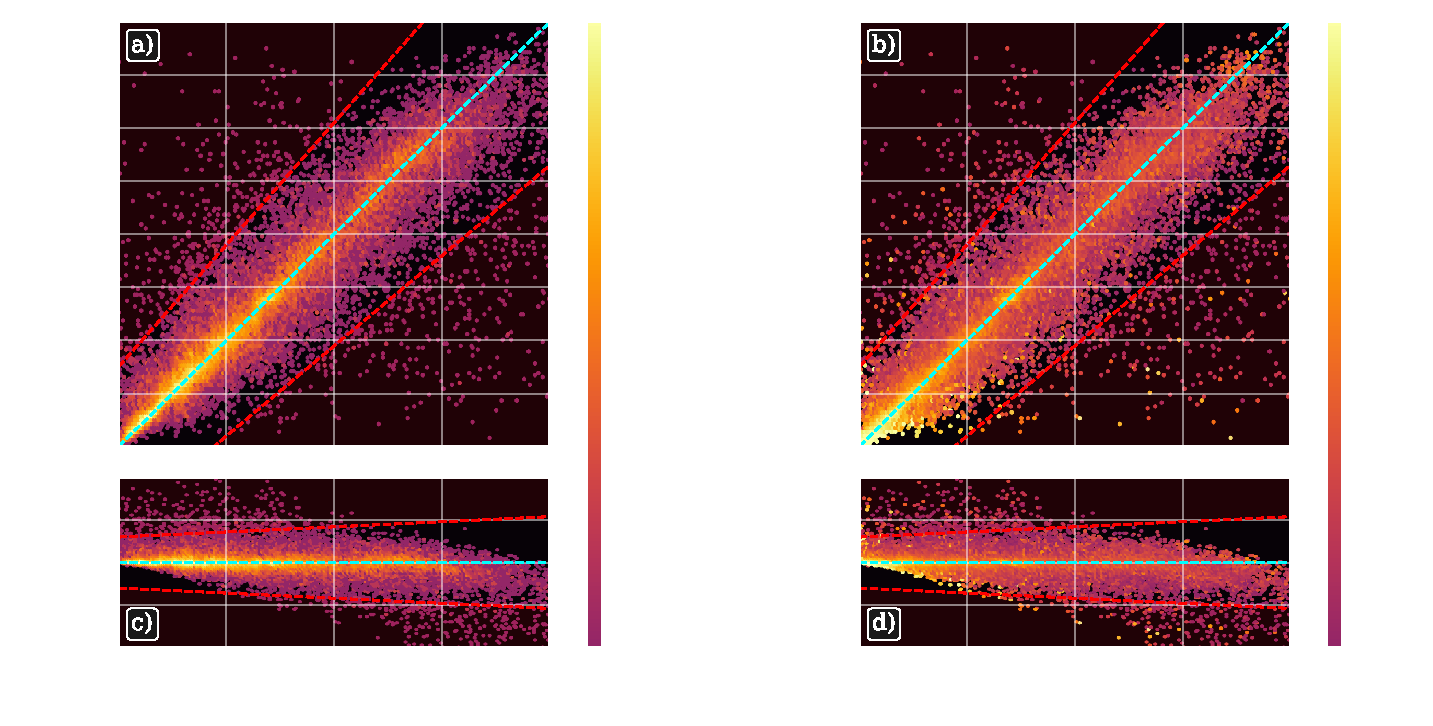
\includegraphics[height=7cm]{script/images/results_scatterplot_residuals.pdf}
    \end{figure}
\end{frame}

\begin{frame}[c]{Redshifts fotométricos: estimativas de ponto único}
    \begin{figure}
        \centering
        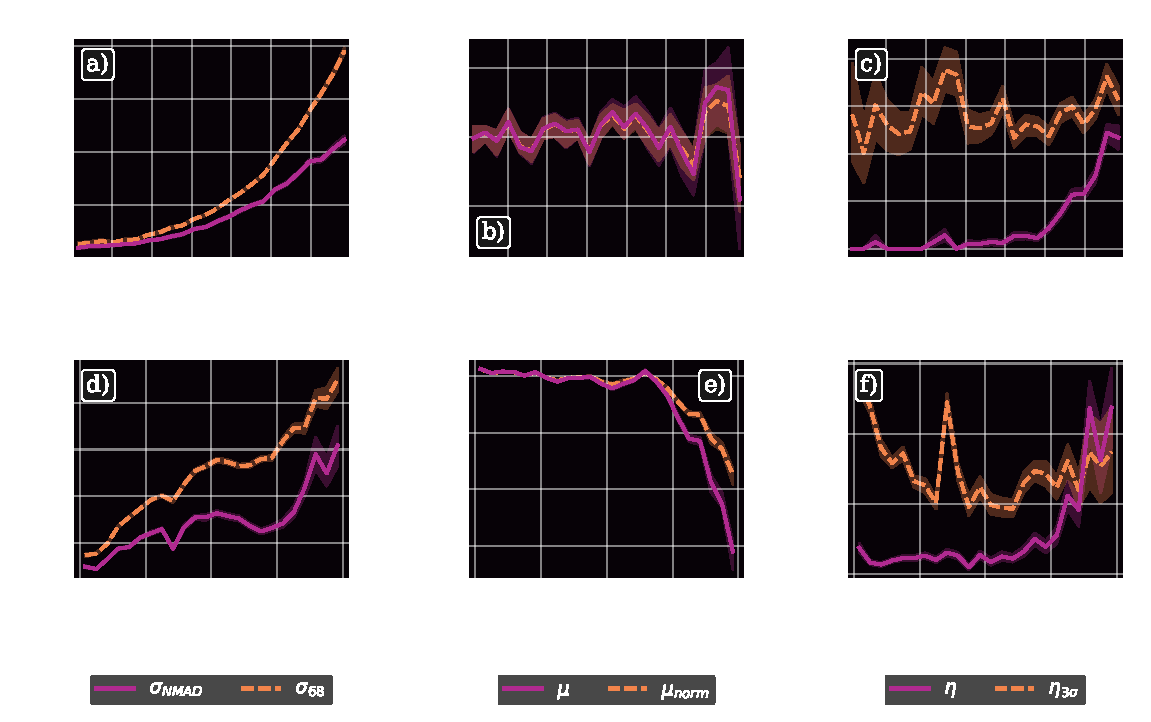
\includegraphics[height=7cm]{script/images/results_spe_metrics.pdf}
    \end{figure}
\end{frame}

\begin{frame}[c]{Redshifts fotométricos: estimativas de ponto único}
    \begin{figure}
        \centering
        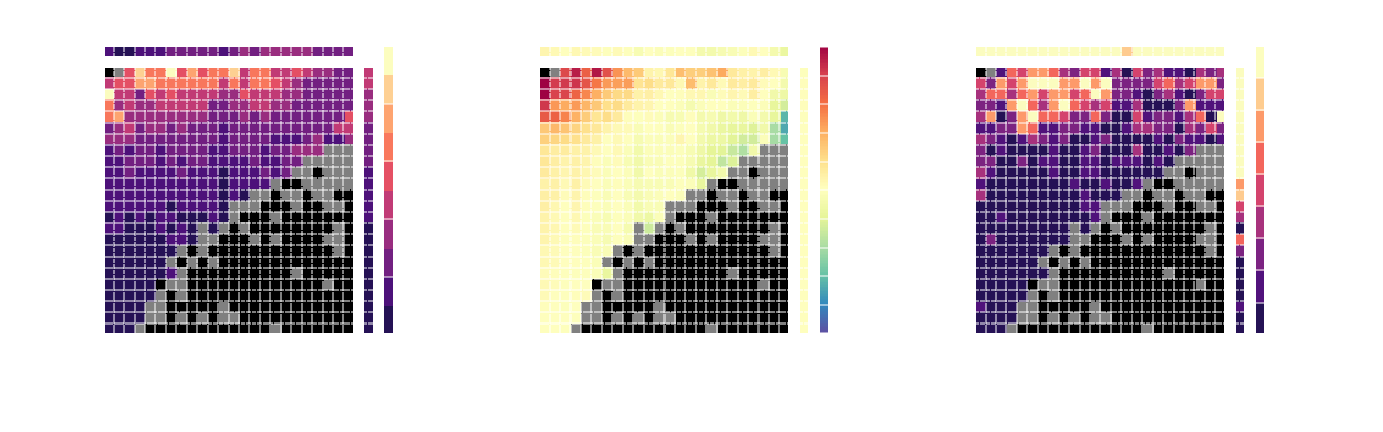
\includegraphics[width=\linewidth]{script/images/results_spe_metrics_2d.pdf}
    \end{figure}
\end{frame}

\begin{frame}[c]{Redshifts fotométricos: estimativas de ponto único}
    Para verificar se a distribuição de photo-zs está como é esperado, comparamos os resultados que obtemos com os resultados de dois outros modelos, um KNN e uma RF, para objetos na Stripe-82.

    \begin{figure}
        \centering
        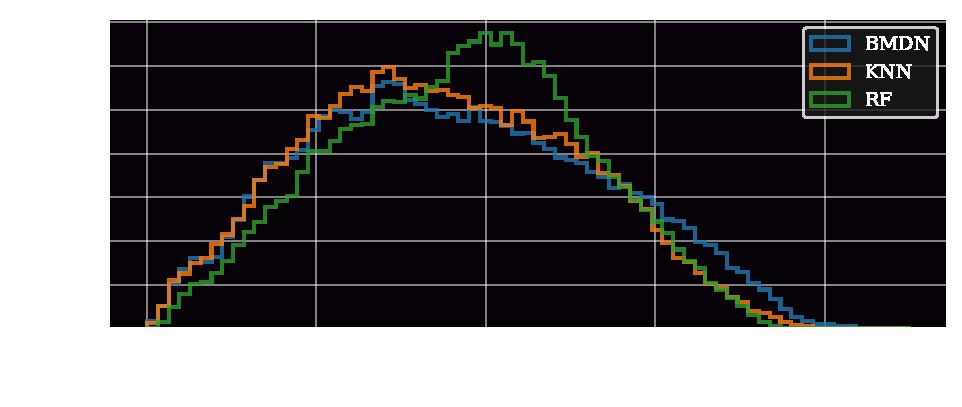
\includegraphics[width=0.8\linewidth]{script/images/s82_redshifts.pdf}
    \end{figure}
\end{frame}

\begin{frame}[c]{Redshifts fotométricos: funções de densidade de probabilidade}
    % \begin{itemize}
    %     \item Odds \textcolor{LightGray}{(Benitez, 2000)}
    %     \item Highest Probability Density Credible Interval \textcolor{LightGray}{(Wittman et al., 2016)}
    %     \item Probability Integral Transform \textcolor{LightGray}{(Polsterer et al., 2016)}
    %     %\item Continuous Ranked Probability Score \textcolor{LightGray}{(Hersbach, 2000; Polsterer et al., 2016)}
    %     \item $\sigma_{68}$ e valor máximo
    % \end{itemize}

    \begin{splusbox}{Odds \textcolor{LightGray}{(Benitez, 2000)}}
        \small
        \vspace{-.5cm}
        \begin{align*}
          \text{odds}_i = \int_{z_\text{peak, $i$}-\Delta z}^{z_\text{peak, $i$}+\Delta z} \text{PDF}_i(z)~\text{d}z,
        \end{align*}
    \end{splusbox}

    \begin{splusbox}{Probability Integral Transform \textcolor{LightGray}{(Polsterer et al., 2016)}}
        \small
        \vspace{-.5cm}
        \begin{align*}
            \text{PIT}_i = \int_{0}^{z_\text{spec}} \text{PDF}_i(z)~\text{d}z = \text{CDF}_i(z_\text{spec}).
          \end{align*}
    \end{splusbox}

    \centering
    \begin{tcolorbox}[hbox]
        \small
        Highest Probability Density Credible Interval \textcolor{LightGray}{(Wittman et al., 2016)}
    \end{tcolorbox}

    \begin{tcolorbox}[hbox]
        \small
        $\sigma_{68}$ e valor máximo
    \end{tcolorbox}

\end{frame}

\begin{frame}[c]{Redshifts fotométricos: funções de densidade de probabilidade}
    \begin{figure}
        \centering
        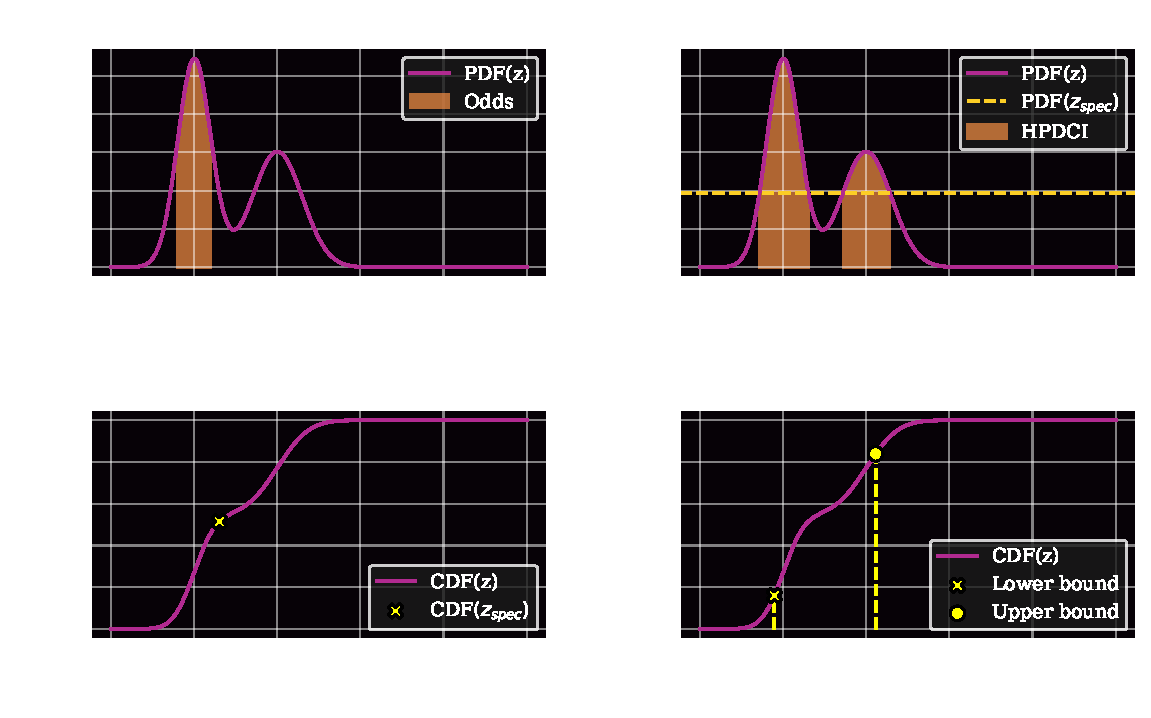
\includegraphics[height=7cm]{script/images/results_pdf_metrics_illust_2.pdf}
    \end{figure}
\end{frame}

% \begin{frame}[c]{Redshifts fotométricos: funções de densidade de probabilidade}
%     PDF: apresentar métricas, histogramas de calibração, resultados por campo
% \end{frame}

\begin{frame}[c]{Redshifts fotométricos: funções de densidade de probabilidade}
    \begin{figure}
        \centering
        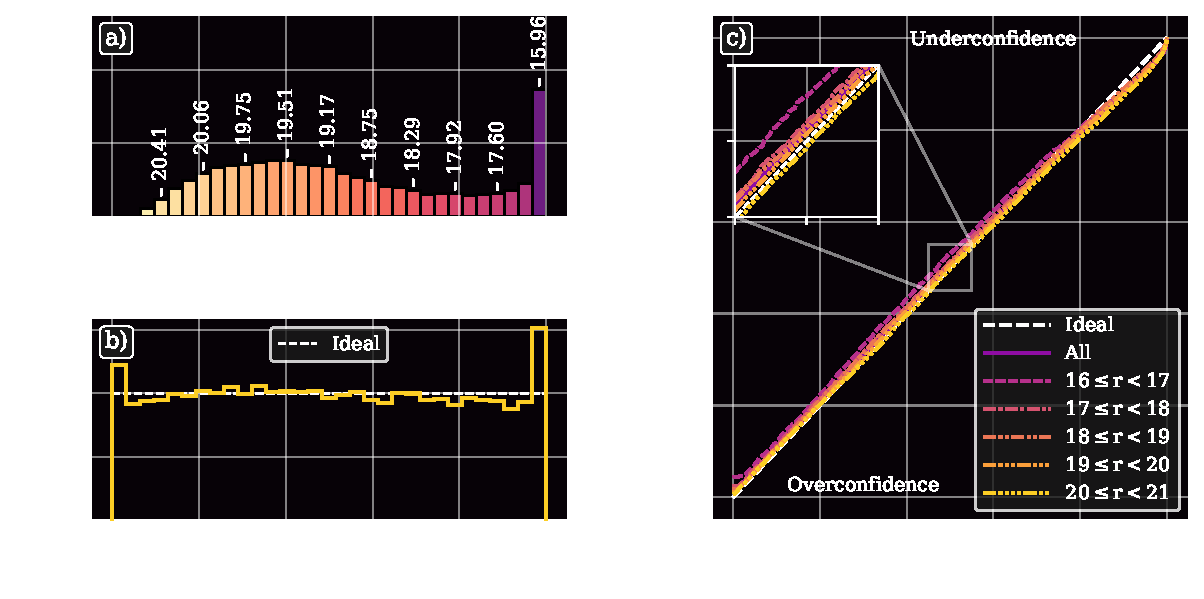
\includegraphics[height=7cm]{script/images/result_pdf_summary.pdf}
    \end{figure}
\end{frame}

\begin{frame}[c]{Redshifts fotométricos: funções de densidade de probabilidade}
    \begin{figure}
        \centering
        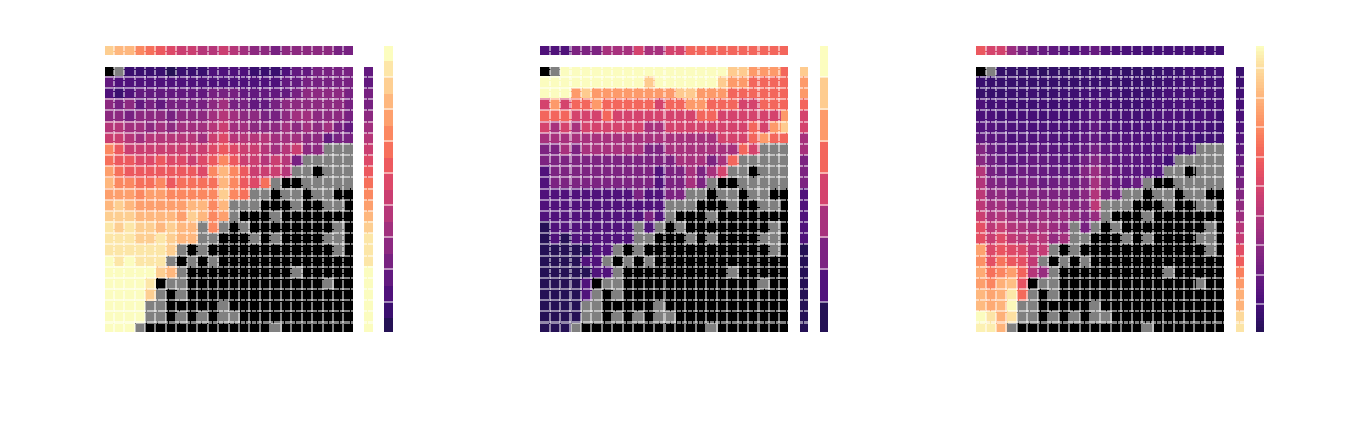
\includegraphics[width=\linewidth]{script/images/results_pdf_metrics_2d.pdf}
    \end{figure}
\end{frame}

\section{Estrutura em larga escala}
\begin{frame}[c]{Estrutura em larga escala}
    \begin{figure}
        \centering
        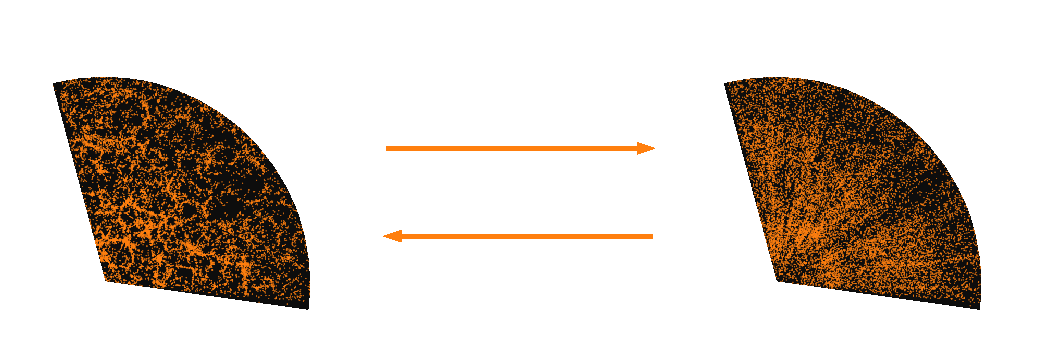
\includegraphics[width=\linewidth]{script/images/lss_problem.pdf}
    \end{figure}
    %
    \centering
    \begin{tcolorbox}[hbox] % <---
        Interpretamos que o $z_\text{phot}$ é igual a $z_\text{spec} + \epsilon$
    \end{tcolorbox}
    % \begin{splusbox}{}
    %     \centering
    %     Interpretamos que o $z_\text{phot}$ é igual a $z_\text{spec} + \epsilon$
    % \end{splusbox}
\end{frame}

% \begin{frame}[c]{Estrutura em larga escala}
%     \begin{splusbox}{Autoencoders e U-Nets}
%         Redes desenvolvidas especificamente para fazer compressão de dados, podendo remover ruído
%     \end{splusbox}

%     \begin{splusbox}{Denoising Diffusion Probabilistic Models (DDPMs)}
%         Redes que utilizam um processo de difusão (e difusão inversa) para aprender uma distribuição que representa os dados, podem ser utilizadas para remover ruído
%     \end{splusbox}

%     \begin{splusbox}{Graph Neural Networks (GNNs)}
%         Redes que utilizam outra estrutura de dados (grafos), e que é capaz de utilizar informação de posição e relação entre amostras para melhorar seus resultados
%     \end{splusbox}
% \end{frame}

\begin{frame}[c]{Estrutura em larga escala}
    \centering
    % \begin{splusbox}{}
    %     \large Autoencoders e U-Nets
    % \end{splusbox}

    % \begin{splusbox}{}
    %     \large Denoising Diffusion Probabilistic Models (DDPMs)
    % \end{splusbox}

    % \begin{splusbox}{}
    %     \large Graph Neural Networks (GNNs)
    % \end{splusbox}

    \begin{tcolorbox}[hbox] % <---
        \large Autoencoders e U-Nets
    \end{tcolorbox}
    \vspace{0.5cm}
    \begin{tcolorbox}[hbox] % <---
        \large Denoising Diffusion Probabilistic Models (DDPMs)
    \end{tcolorbox}
    \vspace{0.5cm}
    \begin{tcolorbox}[hbox] % <---
        \large Graph Neural Networks (GNNs)
    \end{tcolorbox}
\end{frame}

\begin{frame}[c]{Autoencoders {\small \textcolor{LightGray}{(Kramer, 1991; Kingma e Welling, 2013; Ronnerberger et al., 2015)}}}
    \begin{columns}[c]
        \begin{column}{0.36\linewidth}
            \begin{splusbox}{}
                \begin{itemize}
                    \justifying
                    \item São caracterizadas pela existência de um gargalo
                    \item Treinamento simultâneo de duas redes
                    \item Tem como objetivo reproduzir o input com menos informação
                    \item Remove ruído pois ele não é fundamental na reconstrução do input
                \end{itemize}
            \end{splusbox}
        \end{column}
        \begin{column}{0.56\linewidth}
            \begin{figure}
                \centering
                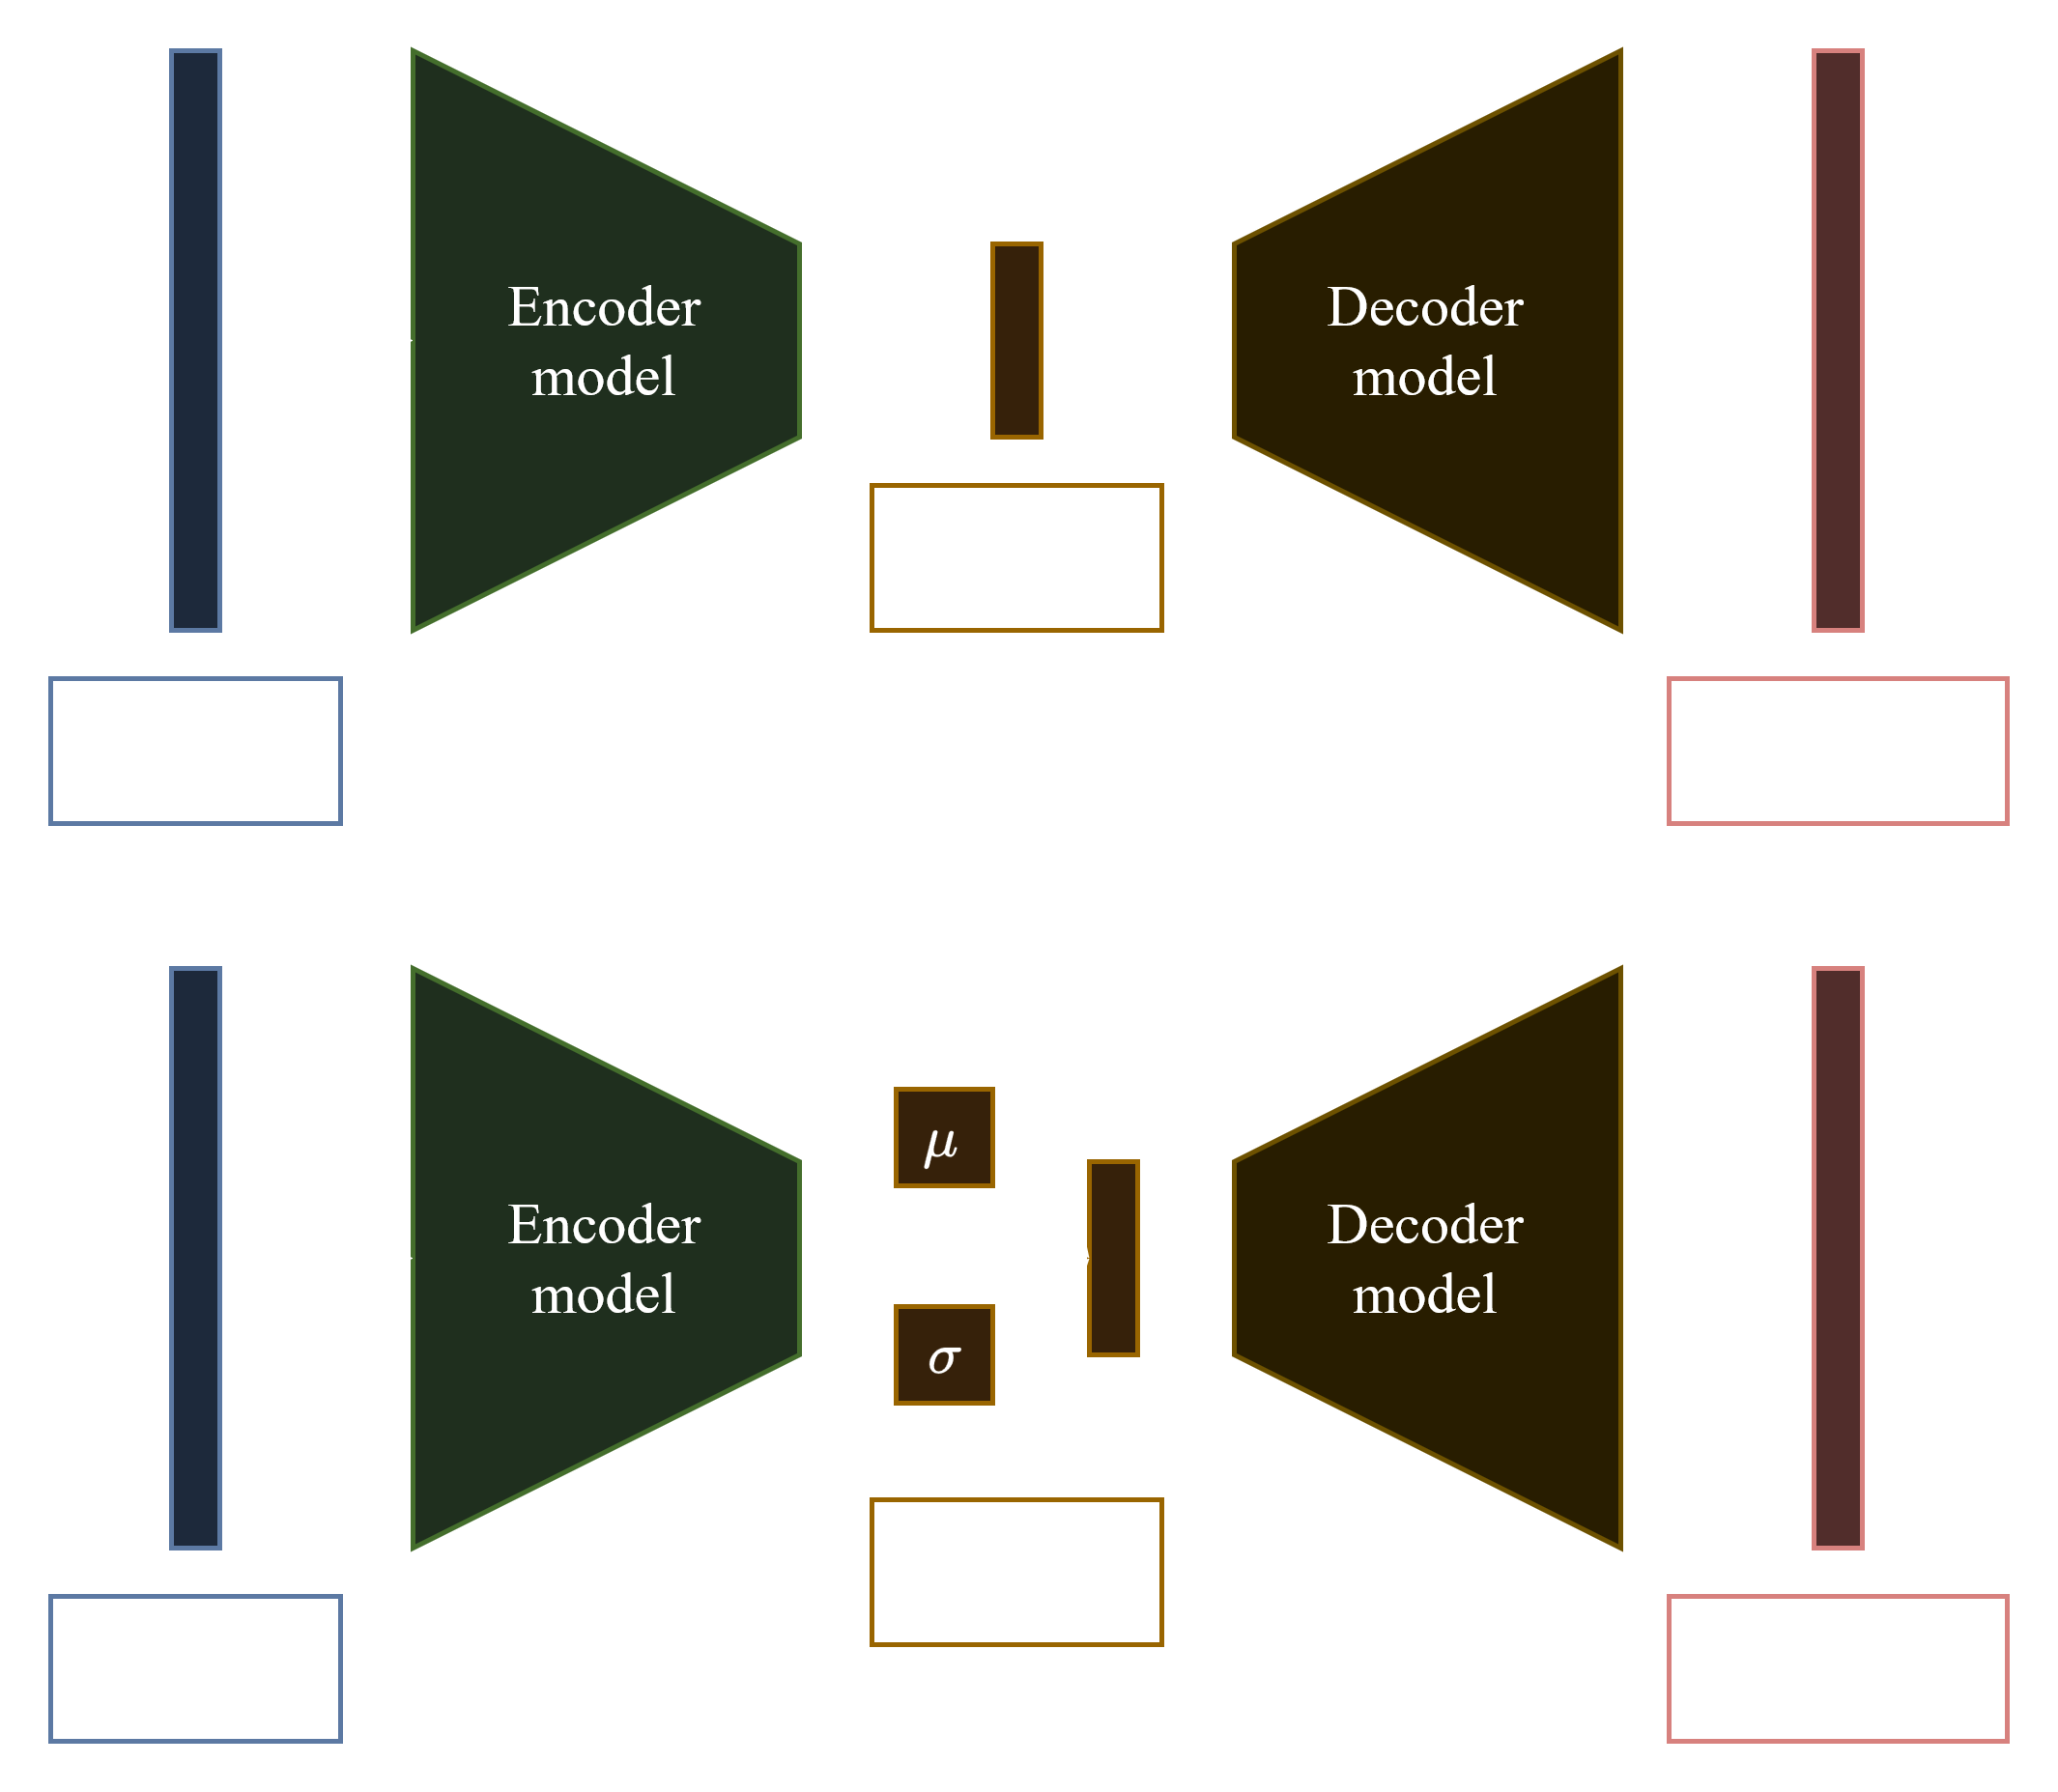
\includegraphics[height=6.5cm]{script/images/autoencoders.png}
            \end{figure}
        \end{column}
    \end{columns}
\end{frame}

\begin{frame}[c]{Autoencoders}
    \begin{figure}
        \centering
        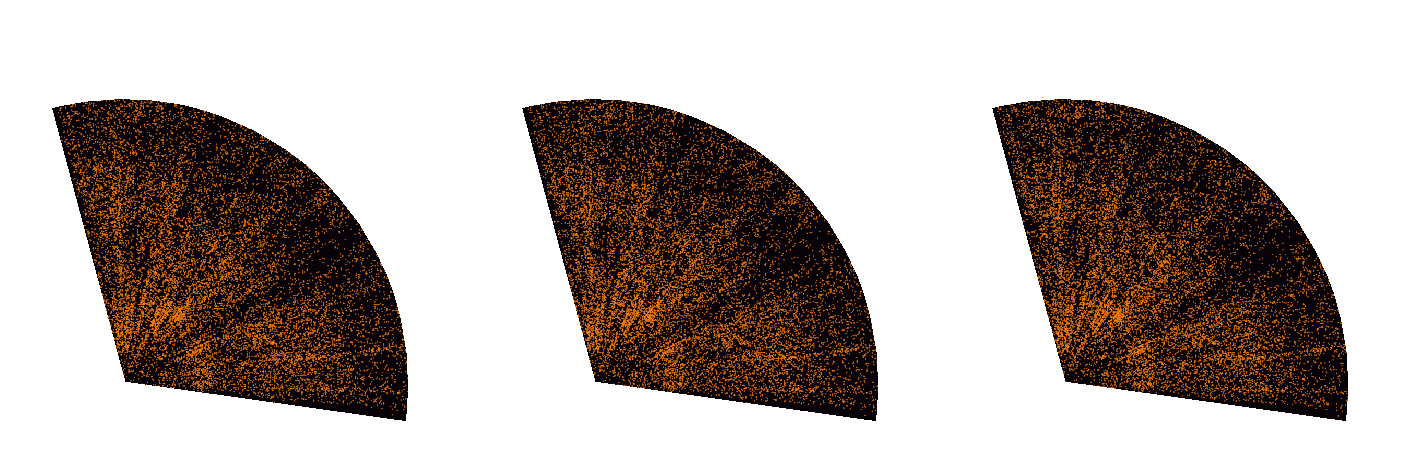
\includegraphics[width=\linewidth]{script/images/redshift_polar_plot_zml_zmlae_zmlvae.pdf}
    \end{figure}
\end{frame}

\begin{frame}[c]{Autoencoders}
    \begin{figure}
        \centering
        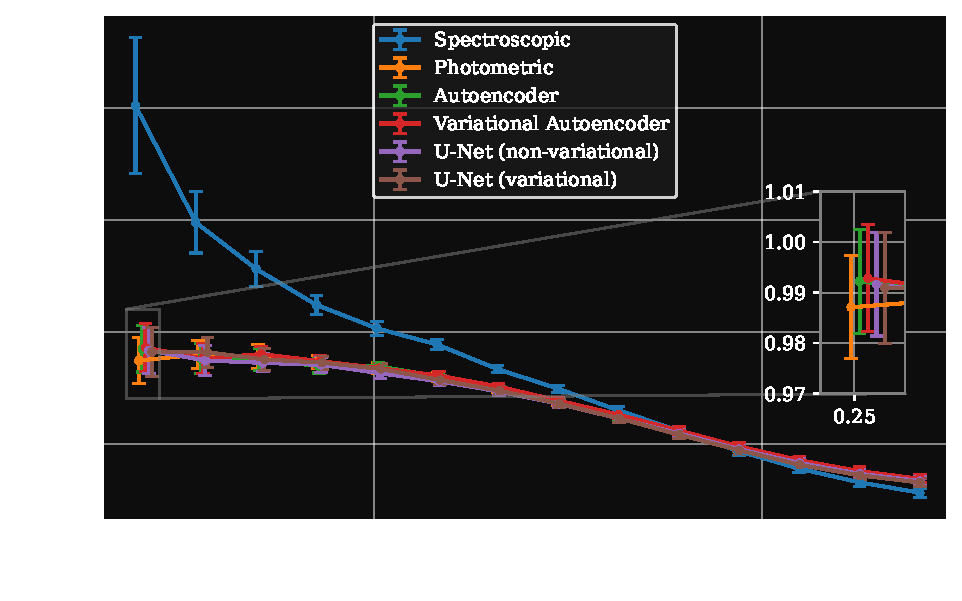
\includegraphics[height=7cm]{script/images/2pcf_compare_corrfunc.pdf}
    \end{figure}
\end{frame}

\begin{frame}[c]{Denoising Diffusion Probabilistic Models  {\small \textcolor{LightGray}{(Ho et al., 2020)}}}
    \begin{figure}
        \centering
        \includegraphics[width=\linewidth]{script/images/diffusion.png}
        \caption{Adaptado de \url{https://cvpr2022-tutorial-diffusion-models.github.io/}.}
    \end{figure}

    \centering
    \begin{splusbox}{}
        É capaz de modelar as incertezas sem suposições simples (por ex. erros são Gaussianos), e pode aprender correlações nas incertezas do photo-z
    \end{splusbox}
    % \begin{tcolorbox}[hbox]
    %     É capaz de modelar as incertezas sem suposições simples (por ex. erros são Gaussianos), e pode aprender correlações nas incertezas do photo-z
    % \end{tcolorbox}
\end{frame}

% \begin{frame}[c]{Denoising Diffusion Probabilistic Models}
%     \begin{splusbox}{}
%         \begin{itemize}
%             \item Modelagem das incertezas como um forward-process
%             \item É capaz de aprender correlações e efeitos não-Gaussianos nas incertezas do photo-z
%             %\item Condicionamento na fotometria, permitindo a obtenção de um photo-z mais próximo ao spec-z diretamente, contornando a necessidade de passos intermediários
%             \item Fornece estimativas probabilísticas
%         \end{itemize}
%     \end{splusbox}
% \end{frame}

\begin{frame}[c]{Denoising Diffusion Probabilistic Models}
    \begin{columns}[c]
        \begin{column}{0.46\linewidth}
            \begin{splusbox}{Tabular}
                \begin{itemize}
                    \item[$\checkmark$] Lida com a estrutura natural dos dados
                    \item[$\checkmark$] Computacionalmente mais leve
                    \item[$\times$] Sem possibilidade de aprender relações espaciais
                    \item[$\times$] Não usa arquiteturas comuns a esse problema
                \end{itemize}
            \end{splusbox}
        \end{column}
        \begin{column}{0.46\linewidth}
            \begin{splusbox}{Imagens}
                \begin{itemize}
                    \item[$\checkmark$] Usa arquiteturas conhecidas (U-Net)
                    \item[$\checkmark$] Aprenderia relações espaciais
                    \item[$\checkmark$] Entendimento mais simples
                    \item[$\times$] Computacionalmente mais pesado
                    \item[$\times$] Modifica a forma natural dos dados
                \end{itemize}
            \end{splusbox}
        \end{column}
    \end{columns}
\end{frame}

\begin{frame}[c]{Denoising Diffusion Probabilistic Models}
    \begin{figure}
        \centering
        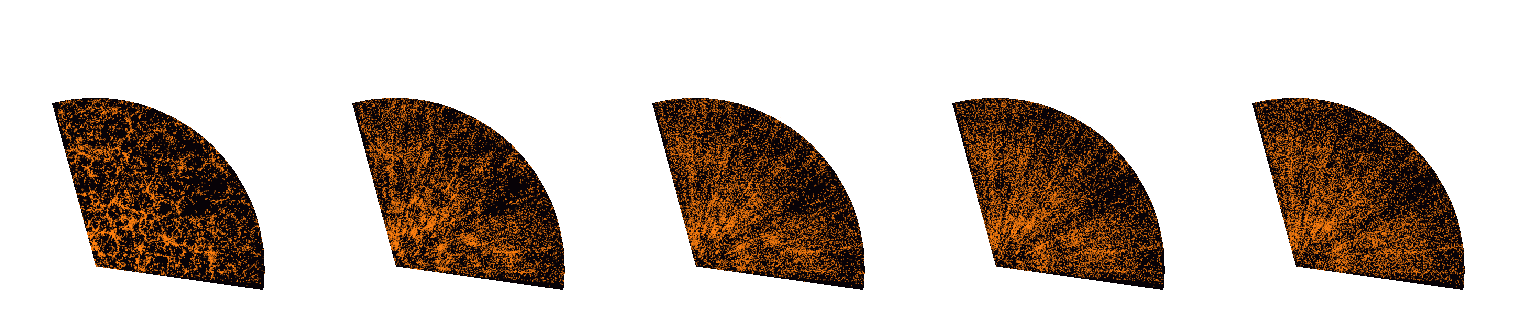
\includegraphics[width=\linewidth]{script/images/lss_illustration.pdf}
    \end{figure}
    %
    \begin{splusbox}{}
        \begin{itemize}
            \item O ruído é modelado de forma que partimos de $z_\text{spec}$ e chegamos em $z_\text{phot}$
            \item O modelo é condicionado na fotometria, dispensando a necessidade de saber o timestep $t$
        \end{itemize}
    \end{splusbox}
\end{frame}

\begin{frame}[c]{Denoising Diffusion Probabilistic Models}
    \begin{figure}
        \centering
        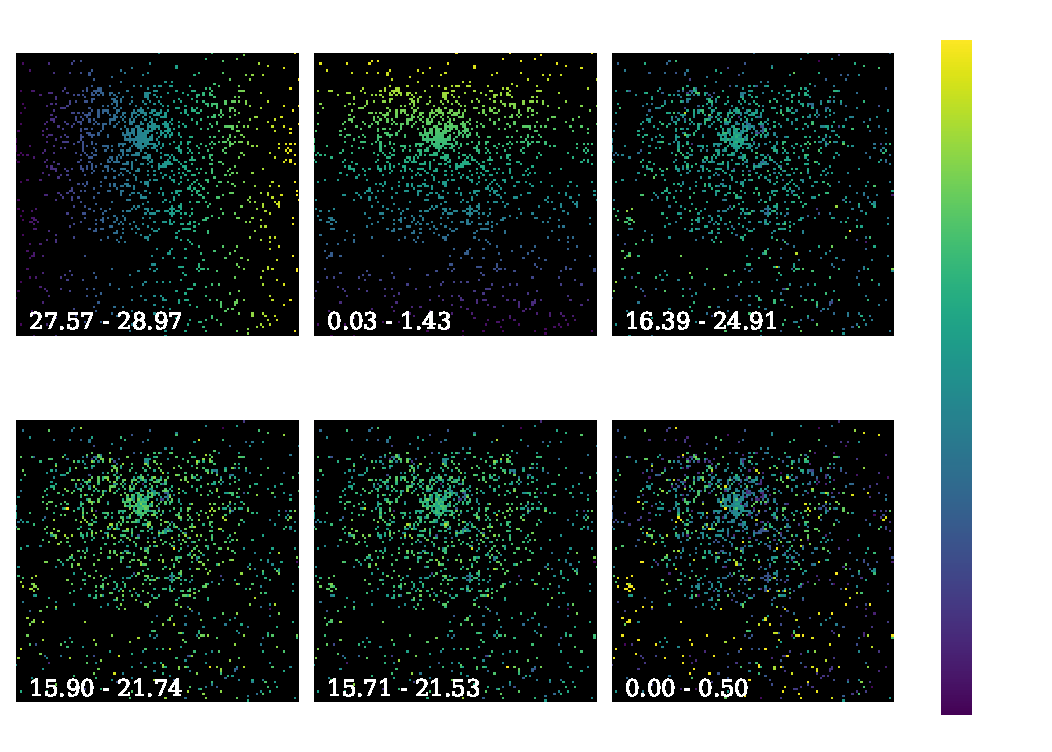
\includegraphics[height=7cm]{script/images/ddpm_diffusion_features.pdf}
    \end{figure}
\end{frame}

\begin{frame}[c]{Denoising Diffusion Probabilistic Models}
    \begin{figure}
        \centering
        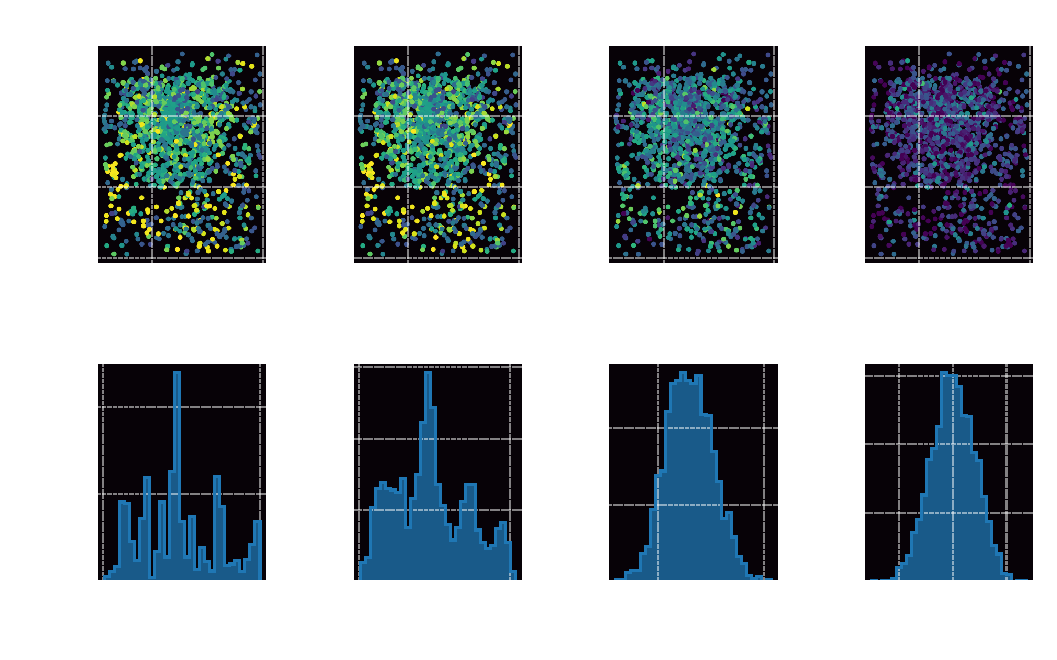
\includegraphics[height=7cm]{script/images/ddpm_diffusion_z.pdf}
    \end{figure}
\end{frame}

\begin{frame}[c]{Graph Neural Networks {\small \textcolor{LightGray}{(Gori et al., 2005; Scarselli et al., 2009)}}}
    \begin{columns}[c]
        \begin{column}{0.46\linewidth}
            \begin{splusbox}{}
                \begin{itemize}
                    \justifying
                    \item Sistemas de recomendação
                    \item Detecção de fraudes
                    \item Descoberta de medicamentos
                    \item Identificação de estruturas de proteínas
                    \item Otimização de cadeias de produção
                \end{itemize}
            \end{splusbox}
        \end{column}
        \begin{column}{0.46\linewidth}
            \begin{figure}
                \centering
                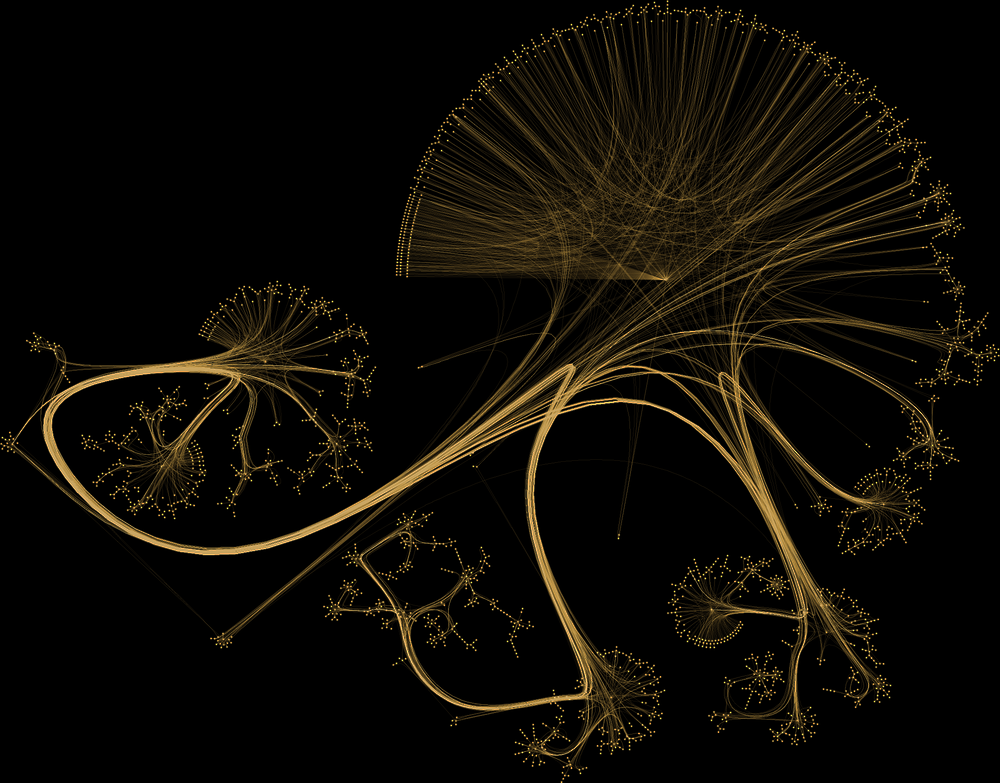
\includegraphics[height=5.5cm]{images/planetoidcora.png}
                \caption{Adaptado de \url{https://graphsandnetworks.com/the-cora-dataset/}}
            \end{figure}
        \end{column}
    \end{columns}
\end{frame}

\begin{frame}[c]{Graph Neural Networks}
    \begin{figure}
        \centering
        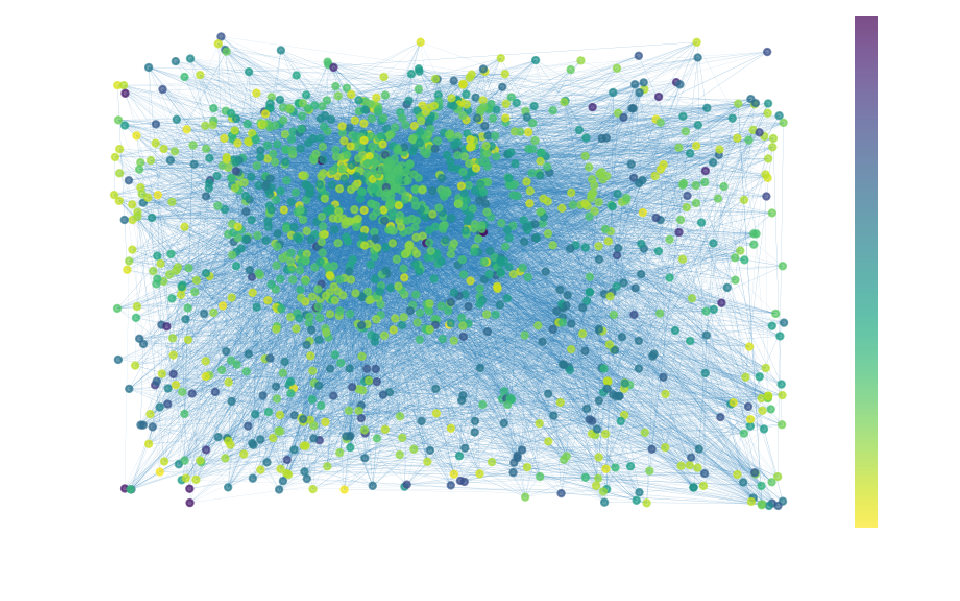
\includegraphics[height=7cm]{images/galaxy_graph.pdf}
    \end{figure}
\end{frame}

\begin{frame}[c]{Graph Neural Networks}
    \begin{figure}
        \centering
        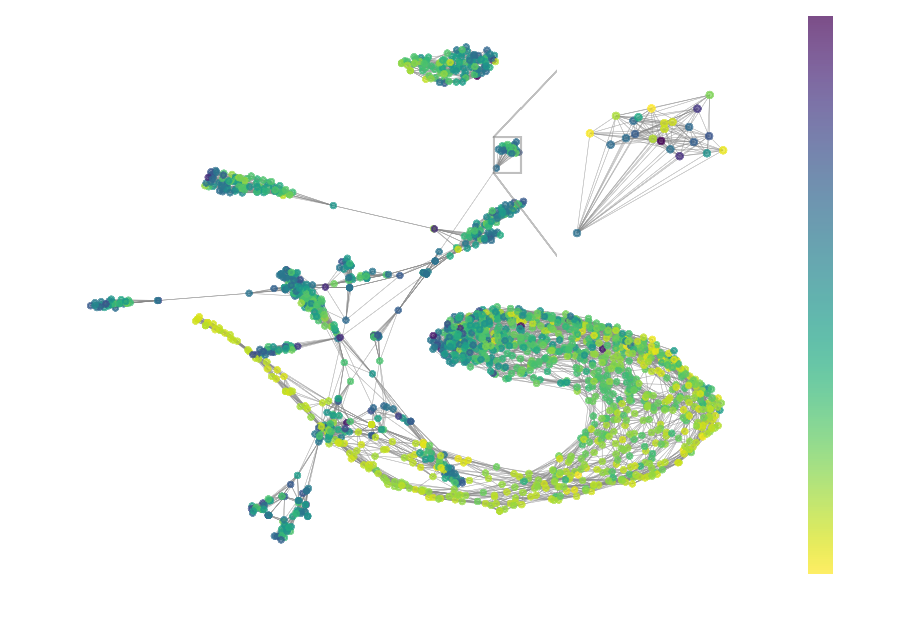
\includegraphics[height=7cm]{images/galaxy_graph_gnn.pdf}
    \end{figure}
\end{frame}

\begin{frame}[c]{Graph Neural Networks}
    \begin{figure}
        \centering
        \includegraphics[width=0.9\linewidth]{images/gnn_message.png}
        \caption{Adaptado de \url{https://snap.stanford.edu/graphsage/}.}
    \end{figure}
\end{frame}

% \begin{frame}[c]{Graph Neural Networks {\small \textcolor{LightGray}{(Gori et al., 2005; Scarselli et al., 2009)}}}
%     \begin{figure}
%         \centering
%         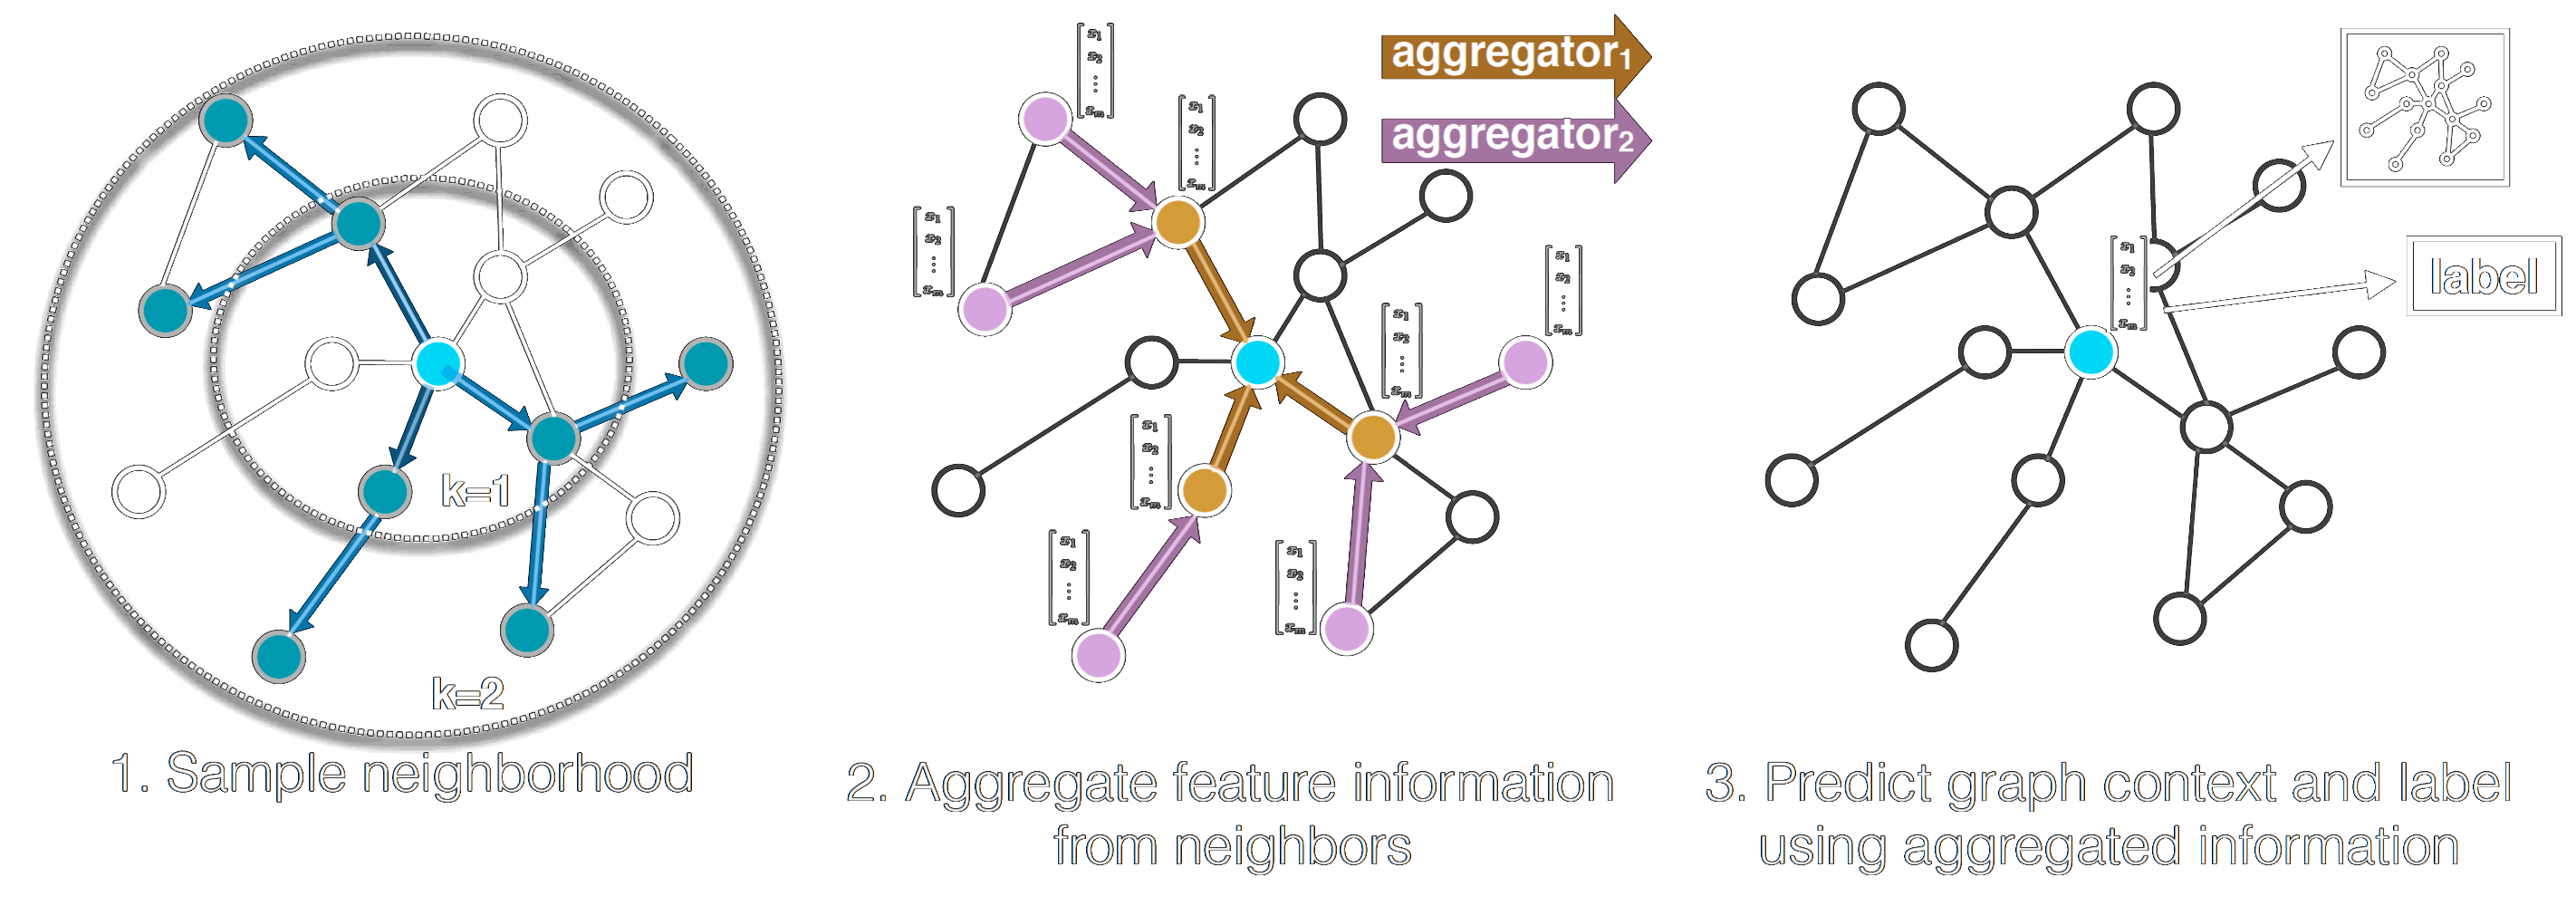
\includegraphics[width=\linewidth]{script/images/sample_and_agg.png}
%         \caption{Adaptado de \url{https://snap.stanford.edu/graphsage/}}
%     \end{figure}
% \end{frame}

% \begin{frame}[c]{Graph Neural Networks}
%     \begin{figure}
%         \centering
%         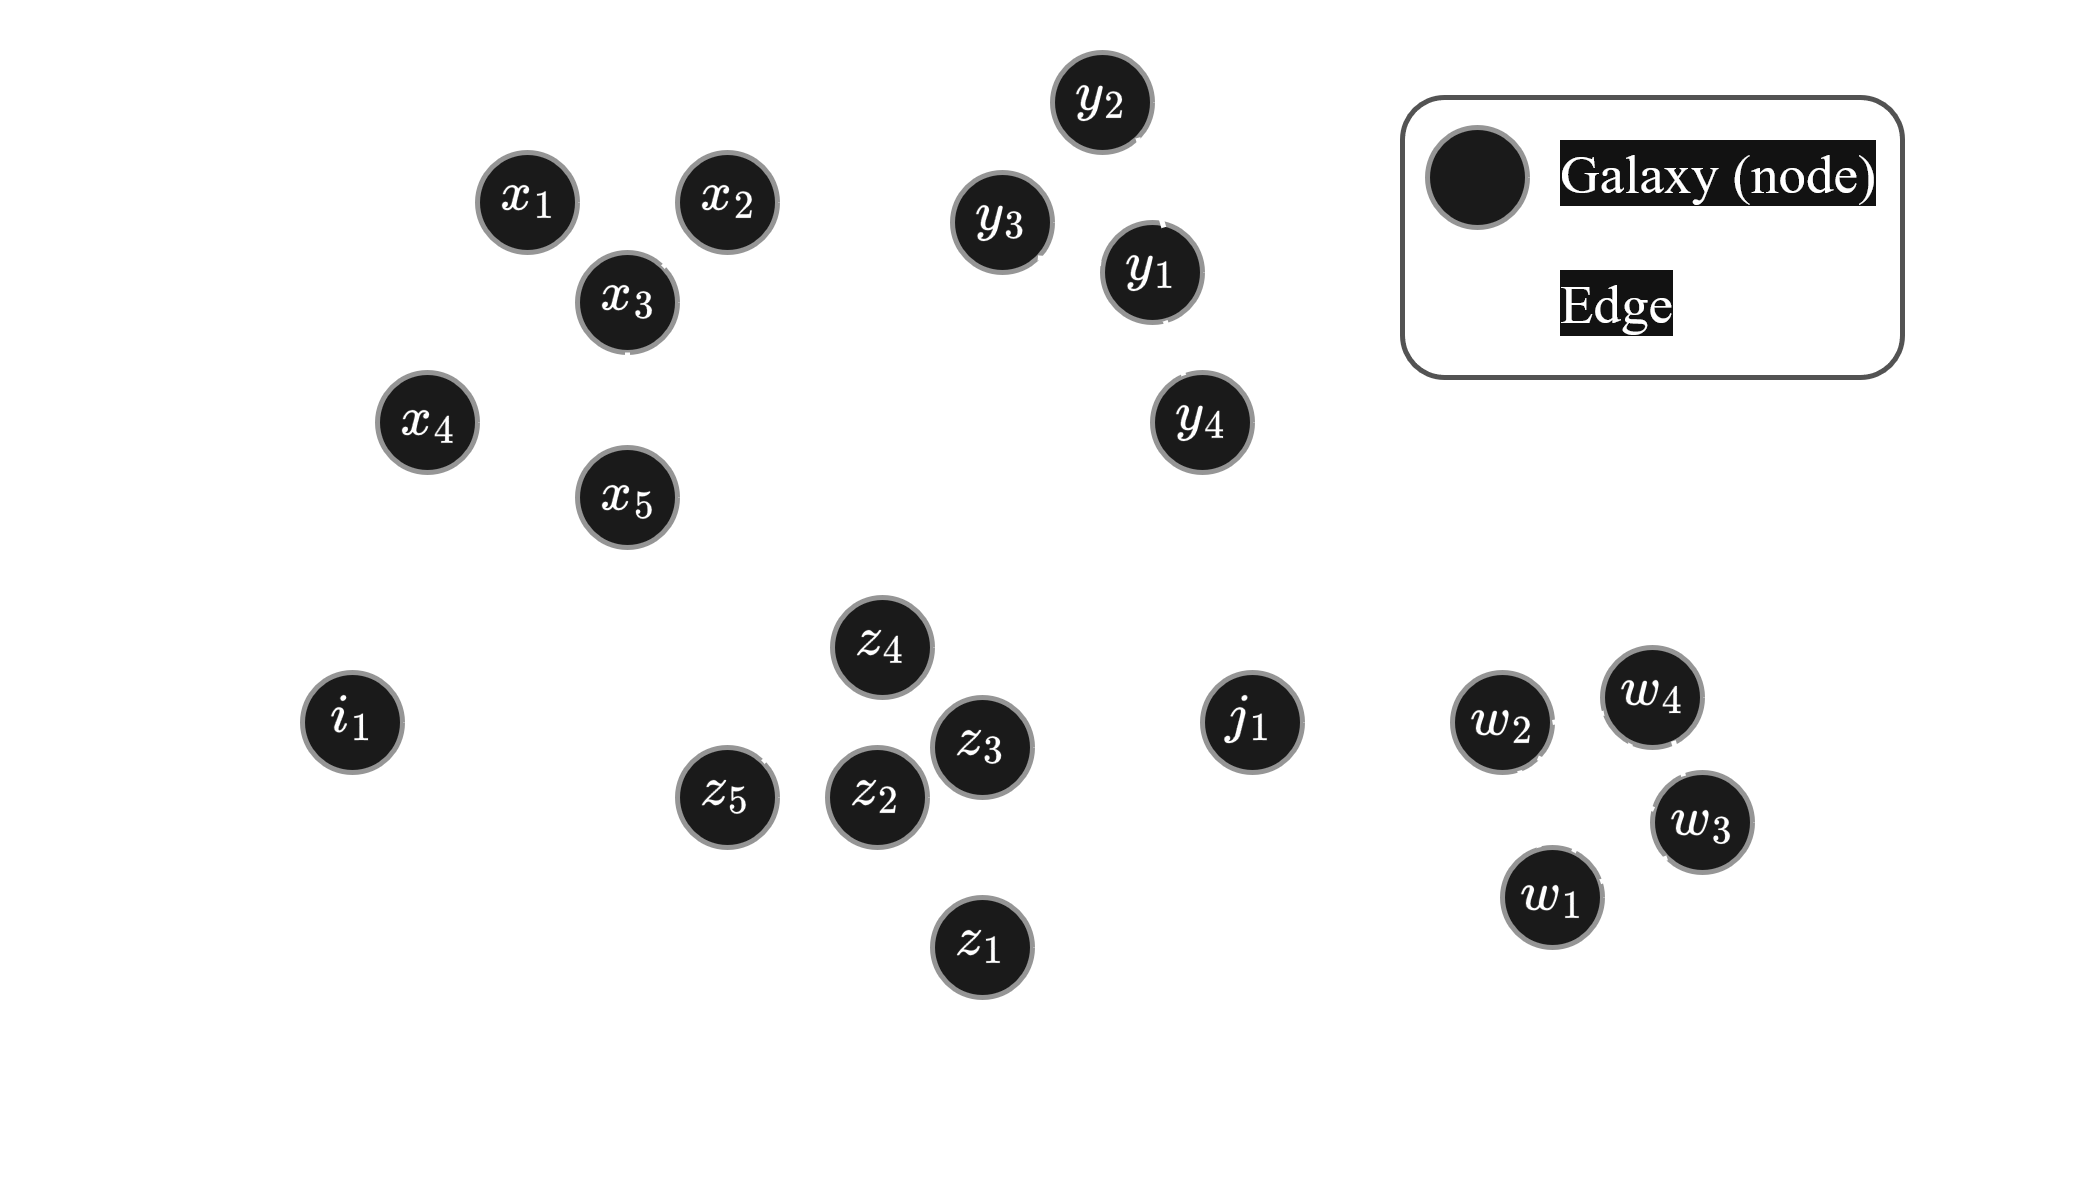
\includegraphics[height=7cm]{script/images/gnn.png}
%     \end{figure}
% \end{frame}

% \begin{frame}[c]{Estrutura em larga escala}
%     \begin{figure}
%         \centering
%         \includegraphics[height=7cm]{script/images/redshift_polar_plot_z_zml.pdf}
%     \end{figure}
% \end{frame}

\section{Conclusões}
% \begin{frame}[c]{Conclusões}
%     \begin{splusbox}{Redshifts fotométricos}
%         \begin{itemize}
%             %\item A estimativa de redshifts fotométricos é fundamental para diversos casos científicos
%             \item O nosso modelo faz estimativas pontuais precisas e acuradas
%             \item Fornece funções de densidade de probabilidade bem calibradas
%             \item Geramos um catálogo com essas informações para toda a colaboração
%         \end{itemize}
%     \end{splusbox}
% \end{frame}

% \begin{frame}[c]{Conclusões}
%     \begin{splusbox}{Redshifts espectroscópicos}
%         \begin{itemize}
%             \item Criamos o maior compilado de redshifts espectroscópicos do Hemisfério Sul
%         \end{itemize}
%     \end{splusbox}

%     \begin{splusbox}{Estrutura em larga escala}
%         \begin{itemize}
%             \item A precisão dos $z_\text{phot}$s serve como ponto de partida para a etapa de recuperação da LSS
%             \item Identificamos possíveis caminhos de progresso (DDPMs, GNNs)
%             \item Este trabalho ainda está em andamento
%         \end{itemize}
%     \end{splusbox}
% \end{frame}

\begin{frame}[c]{Conclusões}
    \small
    \vspace*{0.2cm}
    \begin{splusbox}{Redshifts fotométricos}
        \begin{itemize}
            \setlength\itemsep{.1em}
            %\item A estimativa de redshifts fotométricos é fundamental para diversos casos científicos
            \item O nosso modelo faz estimativas pontuais precisas e acuradas
            \item Fornece funções de densidade de probabilidade bem calibradas
            \item Geramos um catálogo com essas informações para toda a colaboração
        \end{itemize}
    \end{splusbox}
    
    \begin{splusbox}{Redshifts espectroscópicos}
        \begin{itemize}
            \setlength\itemsep{.1em}
            \item Criamos o maior compilado de redshifts espectroscópicos do Hemisfério Sul
        \end{itemize}
    \end{splusbox}

    \begin{splusbox}{Estrutura em larga escala}
        \begin{itemize}
            \setlength\itemsep{.1em}
            \item A precisão dos $z_\text{phot}$s serve como ponto de partida para a etapa de recuperação da LSS
            \item Identificamos possíveis caminhos de progresso (DDPMs, GNNs)
            \item Este trabalho ainda está em andamento
        \end{itemize}
    \end{splusbox}
\end{frame}

\section{Perspectivas futuras}
\begin{frame}[c]{Perspectivas futuras}
    \begin{splusbox}{Redshifts fotométricos}
        \small
        \begin{itemize}
            \item Refatoração do código de forma a simplificá-lo e torná-lo mais eficiente
            \item Desenvolvimento de um código aberto no qual qualquer usuário tem acesso aos modelos e pode fazer estimativas por conta
            \item Aprimoração dos modelos
            \begin{itemize}
                \item Uso de distribuição de magnitudes como input para o treino do modelo
                %\item Criar uma opção de predição determinística
                \item Implementação de uma etapa de template-fitting no processo de treinamento
                %\item Criação de um ensemble
                \item Arquitetura no estilo Mixture-of-Experts/Transformer
            \end{itemize}
        \end{itemize}
    \end{splusbox}
\end{frame}

%\setlength\itemsep{1em}

\begin{frame}[c]{Perspectivas futuras}
    \begin{splusbox}{Compilado espectroscópico}
        \small
        \begin{itemize}
            \item Criar uma nova versão do código que faz o compilado de $z_\text{spec}$, que seja eficiente e fácil de compreender, para divulgação à comunidade.
        \end{itemize}
    \end{splusbox}

    \begin{splusbox}{Estrutura em larga escala}
        \small
        \begin{itemize}
            \item Continuidade nas pesquisas relacionadas à reconstrução da LSS explorando DDPMs e GNNs
            %\item Exploração das metodologias de DDPMs e GNNs, pois ambas apresentam grande potencial para o nosso objetivo
            \item Obtenção da estrutura da LSS reconstruída
            \item Utilizar este resultado como ponto de partida para outras pesquisas
        \end{itemize}
    \end{splusbox}
\end{frame}

\usebeamertemplate{endpage}

\appendix

% \section{Slides extras}

% \begin{frame}[c]{Definindo a arquitetura da rede com o \texttt{Optuna}}
%     \begin{figure}
%         \centering
%         \includegraphics[height=7cm]{script/images/optuna_metrics_boxplots.pdf}
%     \end{figure}
% \end{frame}

% \begin{frame}[c]{Redshifts fotométricos: funções de densidade de probabilidade}
%     \begin{figure}
%         \centering
%         \includegraphics[height=7cm]{script/images/odds_vs_odds_norm.pdf}
%     \end{figure}
% \end{frame}

% \begin{frame}[c]{Redshifts fotométricos: funções de densidade de probabilidade}
%     \begin{figure}
%         \centering
%         \includegraphics[height=7cm]{script/images/results_pdf_average.pdf}
%     \end{figure}
% \end{frame}

% \begin{frame}[c]{Redshifts fotométricos: funções de densidade de probabilidade}
%     \begin{figure}
%         \centering
%         \includegraphics[height=7cm]{script/images/results_pdf_odds_mag_and_z.pdf}
%     \end{figure}
% \end{frame}

% \begin{frame}[c]{Redshifts fotométricos: funções de densidade de probabilidade}
%     \begin{figure}
%         \centering
%         \includegraphics[height=7cm]{script/images/results_pdf_hpdci_mag_z.pdf}
%     \end{figure}
% \end{frame}

% \begin{frame}[c]{Redshifts fotométricos: funções de densidade de probabilidade}
%     \begin{figure}
%         \centering
%         \includegraphics[height=7cm]{script/images/results_pdf_pit_mag_and_z.pdf}
%     \end{figure}
% \end{frame}

% \begin{frame}[c]{Redshifts fotométricos: funções de densidade de probabilidade}
%     \begin{figure}
%         \centering
%         \includegraphics[height=7cm]{script/images/results_pdf_metrics_triangle.pdf}
%     \end{figure}
% \end{frame}